\documentclass[10pt]{article}
\usepackage{titling} % Customize the title
\usepackage[utf8]{inputenc}
\usepackage{eso-pic}
\usepackage{charter}
\usepackage[margin=0.9in]{geometry}
\usepackage{amssymb,pdfpages,fancyhdr,subcaption,graphicx,hyperref,float,outlines,amsmath,gensymb}
\usepackage{listings}
\usepackage{parskip}
\usepackage{multicol} % Added the multicol package
\usepackage{booktabs}
\usepackage{graphicx}
\usepackage{subcaption}
\usepackage{multirow}
\usepackage{listings}
\usepackage{colortbl}

% Define colors for code highlighting
\definecolor{codegreen}{rgb}{0,0.6,0}
\definecolor{codegray}{rgb}{0.5,0.5,0.5}
\definecolor{codepurple}{rgb}{0.58,0,0.82}
\definecolor{backcolour}{rgb}{0.95,0.95,0.92}

% Define settings for Python code
\lstdefinestyle{mystyle}{
    backgroundcolor=\color{backcolour},
    commentstyle=\color{codegreen},
    keywordstyle=\color{blue},
    numberstyle=\tiny\color{codegray},
    stringstyle=\color{codepurple},
    basicstyle=\ttfamily\footnotesize,
    breakatwhitespace=false,
    breaklines=true,
    captionpos=b,
    keepspaces=true,
    numbers=left,
    numbersep=5pt,
    showspaces=false,
    showstringspaces=false,
    showtabs=false,
    tabsize=2
}

\lstset{style=mystyle}

\title{\textbf{4M17 Coursework \#2 \\ Optimisation Algorithm Performance Comparison}}
\author{\textbf{Candidate No: 5730E}}

\begin{document}

\includepdf[pages=-]{Coursework Coversheet.pdf}
\vspace{-3cm}
\maketitle
\begin{multicols}{2}
\section{Introduction}
This report conducts a comparative analysis of two optimisation algorithms applied to minimise Keane's Bump Function, (KBF). In particular, the study focuses on a Continuous Genetic Algorithm, (CGA), as well as an alternative algorithm not covered in the lectures: Parallel Tempering, (PT). The initial sections involve fine-tuning the algorithms on the two-dimensional KBF to enhance their performance and investigate their respective capabilities. Following this, the algorithms are deployed on the eight-dimensional KBF, and a comprehensive performance evaluation is conducted to discern differences and similarities between them. 


The conclusive results indicate that the Continuous Genetic Algorithm excelled in terms of computational efficiency and implementation simplicity, while the Parallel Tempering algorithm showcased superior effectiveness in exploring the solution space and consistently attaining satisfactory solutions. The complete codebase was implemented independently for this study has been provided in Section \ref{sec:code}, as requested, located at the end of the document.
\section{Keane's Bump Function}

To compare the performances of the two algorithms, the Keane's Bump Function, (KBF), is used as the objective function. In particular, the n-dimensional constrained optimisation problem is defined as the maximisation of:

\begin{equation}
    f(\mathbf{x}) = \left| \frac{\sum_{i=1}^{n} (\cos(x_i))^4 - 2\prod_{i=1}^{n} (\cos(x_i))^2}{\sqrt{\sum_{i=1}^{n} i \cdot x_i^2}} \right|
    \label{eq:KBF_cost}
\end{equation}
\begin{equation}
    \begin{aligned}
        \text{subject to} \quad & 0 \leq x_i \leq 10 \quad \forall i \in \{1, \dots, n\} \\
        & \quad \prod_{i=1}^{n} x_i > 0.75 \\
        & \quad \sum_{i=1}^{n} x_i < \frac{15n}{2}
    \end{aligned} 
    \label{eq:KBF_constraints}
\end{equation}

The two-dimensional form of the function has been plotted in Figure \ref{fig:KBF_2D}. Some notable properties are as follows:

\begin{figure}[H]
    \centering
    \begin{subfigure}{0.49\textwidth}
        \centering
        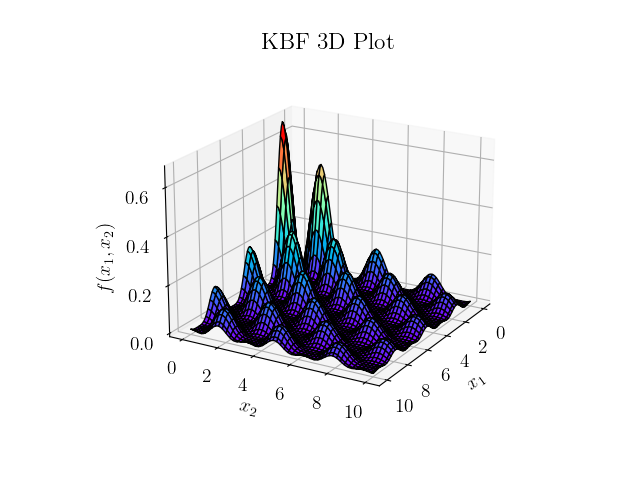
\includegraphics[width=\textwidth]{../figures/KBF/KBF_surf.png}
        \caption{Surface plot.}
        \label{fig:KBF_surf}
    \end{subfigure}
    \begin{subfigure}{0.46\textwidth}
        \centering
        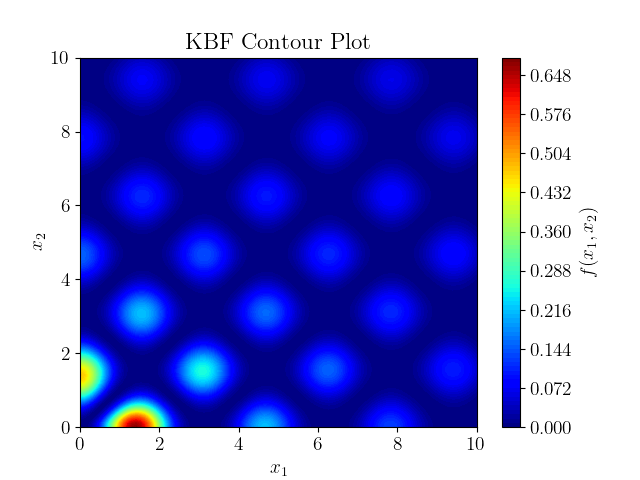
\includegraphics[width=\textwidth]{../figures/KBF/KBF_contour.png}
        \caption{Contour plot.}
        \label{fig:KBF_contour}
    \end{subfigure}
        \captionsetup{justification=centering}
        \caption{Two-dimensional visualisation of the Keane's Bump Function, (KBF).}
        \label{fig:KBF_2D}
\end{figure}

\begin{itemize}
    \item The function is undefined at the origin, (0, 0). This is due to the division by zero in the denominator of Equation (\ref{eq:KBF_cost}). Otherwise, the function is continuous and differentiable everywhere.
    \item The function is highly multi-modal. Its global maximum is located on the boundary $x_{n}=0$, where $x_n$ denotes the final variable in the n-dimensional space. However, there are many local maxima located inside the feasible region, all of which have quite similar amplitudes.
    \item The function is nearly symmetric about the line $x_1=x_2$. This stems from its construction in (\ref{eq:KBF_cost}), using the sums of squared, symmetric terms, $x_i^2$, $(\cos(x_i))^2$, and $(\cos(x_i))^4$. This results in some invariance regarding the order of the input variables. Overall, the peaks consistently manifest in pairs, yet there is a notable pattern wherein one peak always surpasses its counterpart in magnitude.
\end{itemize}

Given the above properties, the KBF is a challenging function to optimise. The presence of multiple, similar-amplitude local maxima makes it difficult for an optimisation algorithm to converge to the global maximum. On the other hand, all control variables share the same nature, (continuous variables), and exhibit identical scales. Additionally, all constraints are of the inequality type, and the feasible space is non-disjoint.

The problem becomes more complicated with the inclusion of the constraints outlined in (\ref{eq:KBF_constraints}). Figure \ref{fig:KBF_Feasible} illustrates the resulting feasible region carved out of the original function space. Notably, the contstraint boundaries are non-linear. The problem complexity is additionally excaberated by the presence of multiple optima along the constraint boundaries, including the global maxima that we seek to identify.

These properties make the KBF a suitable candidate for the comparative analysis of the two optimisation algorithms, as discussed in the previous work of \cite{ELBELTAGY1999639}.

\begin{figure}[H]
    \centering
    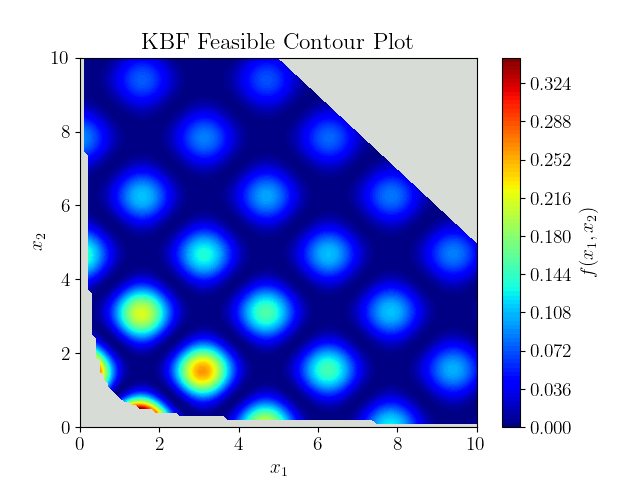
\includegraphics[width=0.48\textwidth]{../figures/KBF/KBF Feasible_contour.png}
    \captionsetup{justification=centering}
    \caption{Feasible region carved out from the two-dimensional visualisation of the Keane's Bump Function, (KBF).}
    \label{fig:KBF_Feasible}
\end{figure}

\section{The Continuous Genetic Algorithm (CGA)}
\label{sec:CGA}

The discrete nature of the Genetic Agorithm, (GA), presented in \cite{parks2023geneticalgorithms} makes it unsuitable for the optimisation of the KBF. An implementation of a Continuous Genetic Algorithm, (CGA), is used instead, which lends itself better to the problems presented in (\ref{eq:KBF_cost})-(\ref{eq:KBF_constraints}).

The CGA, a technique inspired by natural selection and genetics, presents itself as particularly well-suited to tackling challenges associated with multiple local optima. Furthermore, the algorithm lends itself well to parallelisation with low implementation effort, and offers ample opportunities for modifications and adaptations, supported by a rich body of literature on the subject.

The primary difference between the CGA and the GA in \cite{parks2023geneticalgorithms} is the representation of individuals, (solutions of the state space), within the population. Rather than representing an individual as a vector of binary values or bits, (0s and 1s), the CGA uses a real-valued vector of floating-point numbers to represent each individual, as discussed in \cite{PGA}. This allows for a direct representation of the problem, and eliminates the need for a decoding function, which reduces overhead in function evaluations.

This adjustment marks a significant departure from conventional GAs, aligning the algorithm more closely with Evolution Strategies (ES), another member of the evolutionary algorithms family presented in \cite{salimans2017evolution}. However, the algorithm presented in \ref{sec:CGA_implementation} is still classified as a GA in accordance with the differences presented in \cite{10.1007/BFb0029787}, given that mutation does not serve as the primary search mechanism for exploring the state space. Instead, it functions as a non-adaptive, background operator.

\subsection{Implementation}
\label{sec:CGA_implementation}

In accordance with the terminology presented in \cite{parks2023geneticalgorithms}, a vector solution of the state space will be referred to as an \textit{individual} or \textit{chromosome}. Correspondingly, a collection of such individuals arranged in a matrix format will be denoted as a \textit{population}. Each individual is delineated as an $n \times 1$ vector of real-valued (floating-point) numbers, where $n$ signifies the number of variables in the state space. The population itself is represented as a $m \times n$ matrix, where $m$ designates the count of individuals in the population. This count is explicitly defined as a hyperparameter within the code, and is referred to as \textit{POPULATION\_SIZE}.

\begin{figure}[H]
    \centering
    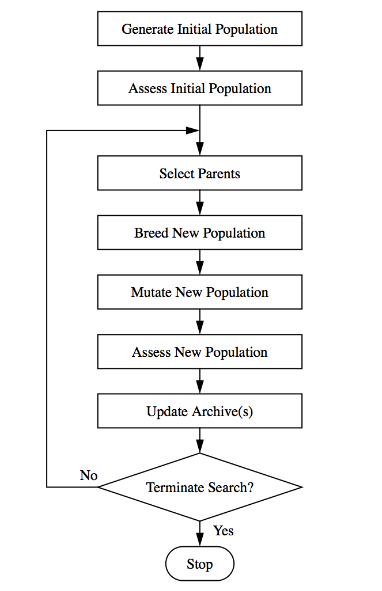
\includegraphics[width=0.46\textwidth]{../figures/Permanent Images/Flowchart.png}
    \captionsetup{justification=centering}
    \caption{A flowchart depicting the CGA process, taken from \cite{parks2023geneticalgorithms}.}
    \label{fig:GAprocess}
\end{figure}

The CGA process is outlined in Figure \ref{fig:GAprocess}. Notably, three selection strategies and two mutation procedures were deliberately implemented to harness the flexibility inherent in the CGA, tailoring it to the optimisation challenges posed by the KBF. The subsequent section, \ref{sec:CGA_selection_mutation}, elucidates the selection method and mutation procedure choices that form the basis of the forthcoming comparison.

The CGA can be can be finely tuned for a specific objective function by modifying its fitness function, which assesses the quality of an individual. The management of constraints is woven into the selection process, as outlined later in Section \ref{sec:CGA_parent_selection}.

\subsubsection{Initialisation}

The population is initialised with random values uniformly distributed within the range of 0 to 10, which represents the bounds of the state space, encompassing both feasible and infeasible values. This population comprises 250 individuals, as defined by the \textit{POPULATION\_SIZE} hyperparameter. 

\subsubsection{Parent Selection}
\label{sec:CGA_parent_selection}

Three selection methods were implemented: proportional selection, tournament selection, and stochastic remainder selection without replacement (SRS). The hyperparameter governing the quantity of parents chosen, denoted as \textit{NUM\_PARENTS}, is established at 25\% of the population size, (rounded down to the nearest even number to facilitate the creation of parent pairs).

Another important aspect of the selection process is the handling of constraints. In particular, the selection process is repeated until only feasible individuals are selected. Infeasible individuals are simply not chosen as parents, a strategy advised by \cite{parks2023geneticalgorithms}, which was deemed suitable considering that the feasible space is non-disjoint, and the constraints are of the inequality type.

\textbf{\underline{Proportional Selection}}

The probability of an individual being selected for mating is proportional to its fitness:
\[
    P_i = \frac{f_i}{\sum_{i=1}^{n} f_i}
\]
Here, \(f_i\) denotes the fitness of the \(i\)th individual. This is the simplest selection method, and is implemented in accordance with the theory presented in \cite{parks2023geneticalgorithms}.

As noted in \cite{parks2023geneticalgorithms}, this approach is susceptible to high variance in individual selection, primarily because there is no assurance of choosing the optimal individual. Alternatively, the following two procedures show greater potential, incorporating a degree of determinism into the selection process.

However, it would be premature to disregard the proportional selection method. There is a chance that the determinism inherent in the other two methods could negatively impact the KBF optimisation process. A notable degree of stochasticity may improve the algorithm's effectiveness in exploring the search space, which may prove vital given the multi-modal nature of the KBF.

\textbf{\underline{Tournament Selection}}

As outlined in \cite{parks2023geneticalgorithms}, this strategy involves taking a small subset of the population, and selecting the top two individuals with the highest fitness. This is repeated until the required number of parents is achieved. Selection pressure can then be adjusted by varying the size of the subset, controlled by the \textit{TOURNAMENT\_SIZE} hyperparameter.

This is a popular selection method, as it is simple to implement, and is known to perform well in practice. It can be improved by including some of the concepts presented in \cite{Miller1995GeneticAT}, however, these have been avoided to reduce the complexity of the algorithm's implementation.

\textbf{\underline{Stochastic Remainder Selection}}\\\vspace{0.5mm}
\textbf{\underline{\hspace{-0.5mm}without Replacement (SRS)}}

This strategy draws inspiration from \cite{parks2023geneticalgorithms}. Specifically, a group of chosen individuals is curated by generating an expected number of copies for each individual, denoted as: 
\[E_i = N * P_i\]
Here, \(N\) represents the population size, and \(P_i\) is elucidated above in the context of proportional selection. The anticipated number of duplicates is subsequently divided into an integer part, \(I_i = \lfloor E_i \rfloor\), and a remainder, \(R_i = E_i - I_i\). 

The integer part is used for deterministic selection of individuals. The $i$th indivdual is selected $I_i$ times. Subsequently, the remained, $R_i$, is then used to stochastically augment the collection of individuals until the required number of parents is achieved. This is done by selecting the $i$th individual with a probability of $R_i$.

The discussion in \cite{parks2023geneticalgorithms} highlights that this approach appears to yield superior performance, ascribed to the inclusion of a degree of determinism in the selection criteria. Nevertheless, it remains worthwhile to evaluate the performance of the other two methods, as they might present distinct advantages within the framework of the KBF.

\subsubsection{Mating Procedure}

Similarly, two mating procedures have implemented: crossover and heuristic crossover. The entire population is replaced by offspring, bred from two randomly allocated parents from the pool of selected parents.

\textbf{\underline{Crossover}}

The crossover procedure adheres to the principles detailed in \cite{parks2023geneticalgorithms}. Initially, a crossover point is randomly chosen. Genes from the first parent are incorporated into the offspring until this point, beyond which genes from the second parent take their place. Specifically, the sequencing of the parents is governed by the probability specified by the hyperparameter \textit{CROSSOVER\_PROB}.

\textbf{\underline{Heuristic Crossover}}

Heuristic crossover is presented in \cite{Michalewicz_2011}. By this variation, a random number $\beta$ in the interval $[0, 1]$ is generated. The genes of the offspring are then determined as a blend of the original two parents, $p_1$ and $p_2$, as follows:
\[
    o_i = \beta (p_{1i} - p_{2i}) + p_{2i}
\]
With this inspiration in mind, heuristic crossover was implemented in the CGA. Specifically, the sequence of parents in the above formula is determined by the \textit{CROSSOVER\_PROB} hyperparameter, aligning with the approach used previously in the original crossover procedure.

A crucial factor to bear in mind is that certain offspring may be produced outside the feasible region. This implementation deviates from the recommendation in \cite{Michalewicz_2011} by not outright rejecting these offspring during the mating procedure. Rather, they are simply excluded from consideration as parents in the subsequent selection process.

The decision to incorporate this mutation procedure stems from the continuous nature of the state space. While the conventional crossover methods may be well-suited to binary representations, a more intuitive approach emerges when grappling with real-valued variables - using a blend of characteristics from both parents.

Moreover, the use of the heuristic crossover method aims to address previous limitations associated with standard crossover. Unlike conventional crossover, which confines offspring values to those of the parents, blending permits the generation of offspring beyond the parent values, allowing for potentially new information. This feature may prove particularly advantageous in the context of the KBF, enhancing the algorithm's capability to navigate the search space adeptly and thoroughly explore local optima.

An additional noteworthy observation is that the introduction of $\beta$ serves to bring the CGA into closer alignment with Evolutionary Strategies (ES). This resemblance becomes evident as the formulation above bears some similarity to the intermediate recombination strategy outlined in \cite{salimans2017evolution}. Nevertheless, it is essential to emphasise, as mentioned earlier, that mutation does not serve as the primary search mechanism in the CGA. Consequently, the CGA can still be appropriately categorised as a GA, as per the classification seen in \cite{10.1007/BFb0029787}.

\subsubsection{Mutation}

The mutation procedure proposed by \cite{PGA} involves perturbing a gene within a chromosome by a normally distributed random number with a mean of zero and a standard deviation of $\sigma$. However, the effectiveness of this procedure is constrained by the selection of $\sigma$ as an additional hyperparameter, necessitating careful tuning. 

Instead, a simpler approach was adopted, where genes within the population have a probability, given by the mutation rate, of being reset to a random value drawn from a uniform distribution within the confines of the state space, mirroring the initialisation procedure.

\subsubsection{Evaluation}

The population is then evaluated, and the individuals are ranked in order of fitness. Here, the fitness is defined as the negative of the KBF cost function, outlined in (\ref{eq:KBF_cost}). This is done to align the algorithm with the maximisation of the KBF.

\subsubsection{Termination}

For this section of the report, the algorithm terminates after a maximum number of iterations, (defined as a hyperparameter). A more stringent convergence criterion is adopted for the comparison between the two algorithms in Section \ref{sec:CGA_QEG_comparison}. The individual with the lowest fitness value is then returned as the optimal solution to the optimisation problem.

\subsection{Tuning the CGA}
\label{sec:CGA_selection_mutation}

Given the flexibility of the CGA, multiple selection methods and mutation procedures were implemented within the codebase, as discussed previously. These are then selected as hyperparameters within the experiments presented in listing \ref{CGA_TuningExperimentspy}, to take advantage of the flexibility offered by the CGA. 

To choose a selection method and mutation procedure going forwards into the main comparison of this report, listing \ref{CGA_TuningExperimentspy} was used as a platform for experimentation. Each selection method and mutation procedure was evaluated over 10 and 100 iterations, with a constant mutation rate of 0.05, and a crossover probability of 0.7. The number of parents was established at 25\% of the population size, (rounded down to the nearest even number to facilitate the creation of parent pairs). The population size itself was set at 250, and the tournament size was similarly defined as 25\% of this.

Supplementary results regarding this initial exploration of hyperparameter tuning are detailed in Section \ref{sec:CGA_tuning_results}. Specifically, the final fitness values are outlined in Table \ref{tab:CGAexploration}. At a first glance, it would appear that all selection methods and mutation procedures perform similarly, offering convergences to similar fitness values. Minor variations could be attributed to the stochastic nature of the CGA, and the small number of iterations.
\vspace{-1mm}
\begin{figure}[H]
    \centering
    \begin{subfigure}{0.46\textwidth}
        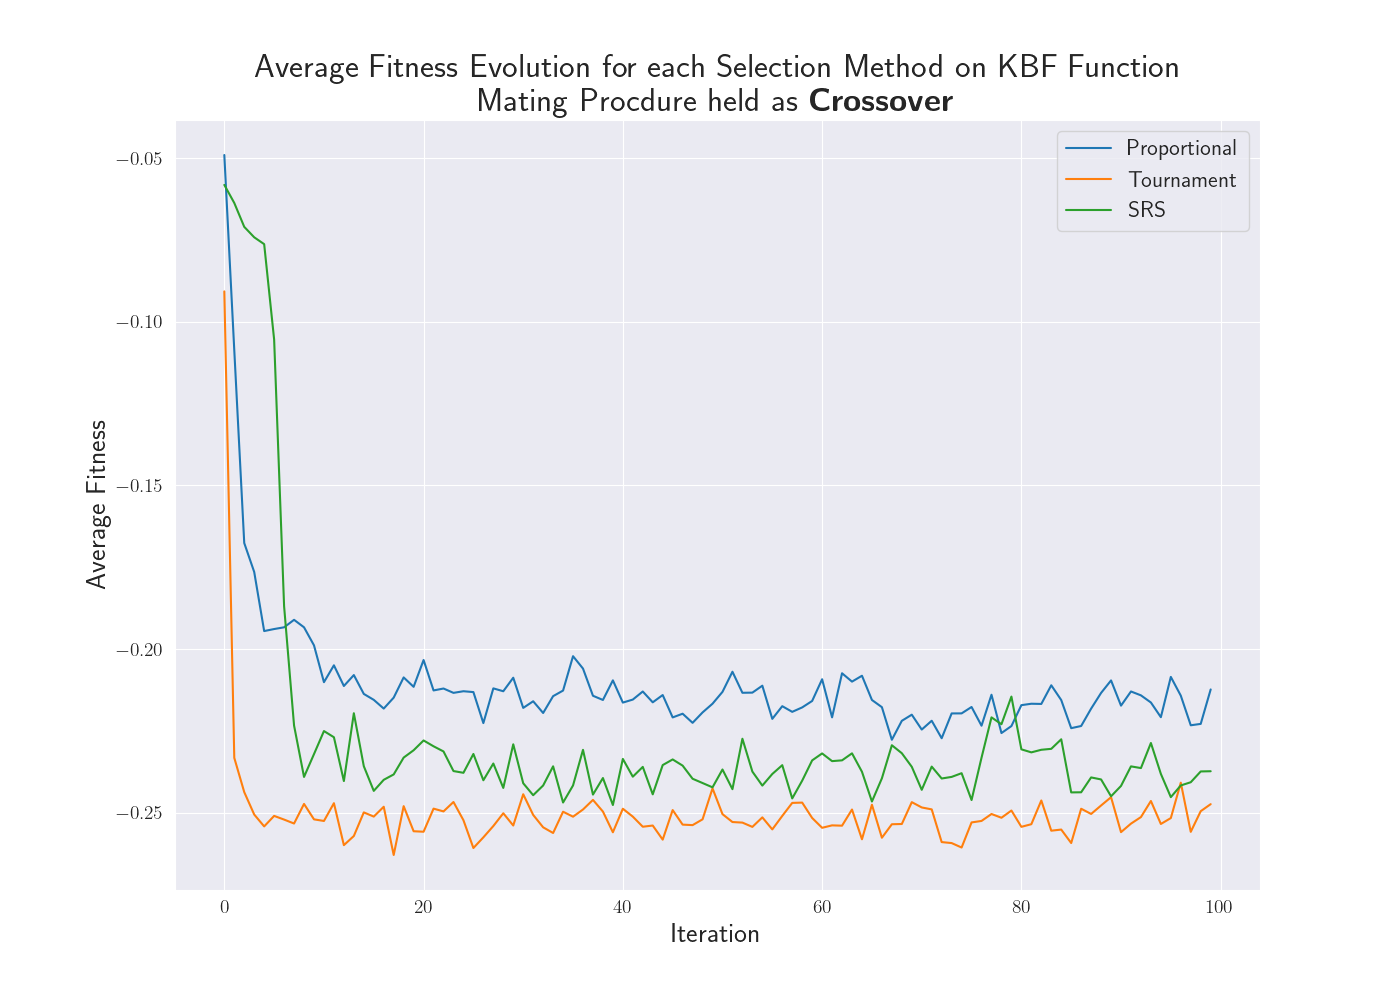
\includegraphics[width=\textwidth]{../figures/Permanent Images/Fitness_Evolution_Crossover.png}
        \caption{Mutation Procedure: Crossover}
        \label{fig:CGA_fitness_evo_Crossover}
    \end{subfigure}
    \begin{subfigure}{0.46\textwidth}
        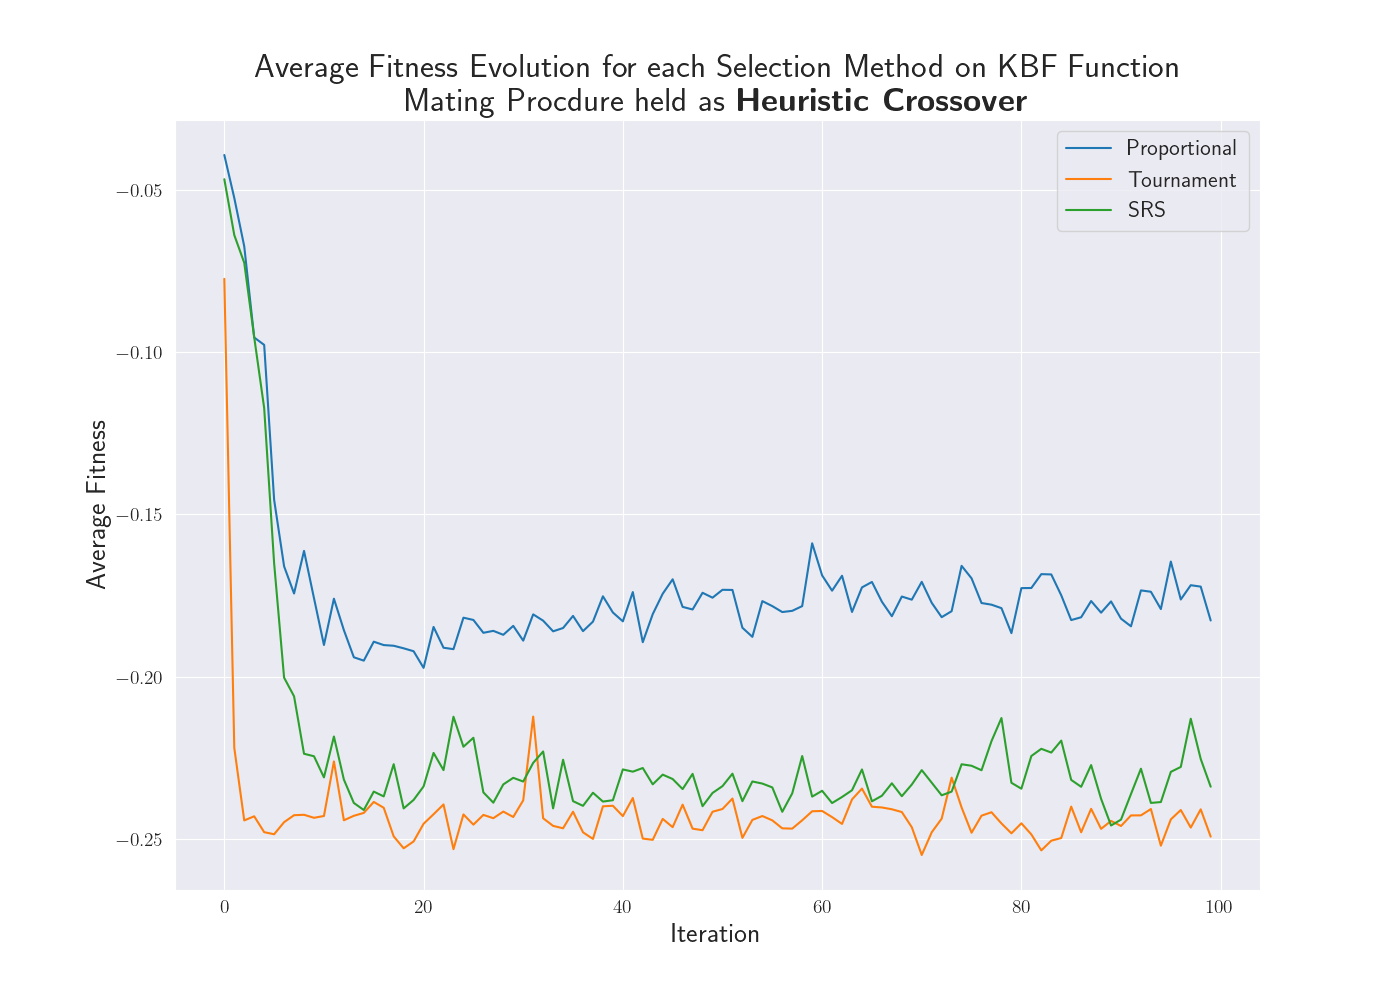
\includegraphics[width=\textwidth]{../figures/Permanent Images/Fitness_Evolution_Heuristic Crossover.png}
        \caption{Mutation Procedure: Heuristic Crossover}
        \label{fig:CGA_fitness_evo_Heuristic Crossover}
    \end{subfigure}
    \captionsetup{justification=centering}
    \caption{Evolution of the average fitness values of the CGA population over 100 iterations for each of the selection methods. The results are presented for both mutation procedures: crossover and heuristic crossover. Here, the mutation rate was set to 0.05, and the crossover probability was set to 0.7.}
    \label{fig:CGA_fitness_evo}
\end{figure}
\vspace{-2mm}
However, more insightful conclusions can be drawn from the figures presented in \ref{fig:CGA_fitness_evo}, which illustrate the rapid evolution of the average fitness values of the CGA population over 100 iterations for each of the selection methods. They illustrate that tournament selection seemed to outperform the other two selection methods when maximising the KBF, which is surprising given the favourable description in \cite{parks2023geneticalgorithms} regarding SRS. 

The experiment was repeated several times, yielding results that were admittedly variable, attributed to the inherent stochastic nature of the CGA. At times, the superiority of SRS over tournament selection was evident, yet proportional selection generally did not prove to perform better. Despite this variability, the outcomes exhibited sufficient consistency to justify the designation of tournament selection as the primary method for the upcoming comparison.

The observed differences in performance may be attributed to the distinct characteristics of the KBF. Tournament selection appears to demonstrate greater efficacy in navigating the search space compared to SRS, perhaps due to its less deterministic nature. This becomes particularly significant in light of the multi-modal nature of the KBF, where a certain level of stochasticity may prove essential for thorough exploration of the search space.

The results additionally indicate that when combined with tournament selection, the heuristic crossover procedure generally outperformed the standard crossover method. This is evident in the typically steeper decline in average fitness values, as illustrated in Fig. \ref{fig:CGA_fitness_evo_Heuristic Crossover}. Furthermore, the heuristic crossover exhibited greater result consistency across repeated experiments and generally converged to higher maximas compared to the standard crossover. Although the observed differences were note always significant, the overall trend supports the choice of heuristic crossover as the preferred mating procedure for the forthcoming comparison.

This may be attributed to the heuristic crossover's capacity to generate offspring beyond the existing genotypes present within a generation. This attribute is especially beneficial within the framework of the KBF, enhancing the algorithm's ability to navigate the search space adeptly and systematically explore the numerous local optima.

Having cemented the selection method and mutation procedue choices as tournament selection and heuristic crossover respectively, the CGA was further tuned to optimise its performance. 

Specifically, choices for the mutation rate and crossover probability were explored. The results are presented in Figure \ref{fig:CGA_contour_rates}, which showcases two heat maps of the final fitness values after 100 iterations for the CGA using the chosen procedures. The plots are presented for both the final average fitness, as well as the final fitness of the best individual.

Notbaly, as depicted in Fig. \ref{fig:CGA_contour_tournament_Heuristic Crossover_AVG}, it is evident that an increased stochasticity of the CGA, indicated by higher crossover probabilities, leads to improved average final fitness. This aligns with expectations, as a broader and more randomly distributed population enhances the likelihood of individuals being situated in the proximity of local maxima. Consequently, a greater number of individuals within the population receive lower fitness values, a trend reflected in the observed average final fitness.

\columnbreak

Fig. \ref{fig:CGA_contour_tournament_Heuristic Crossover_MIN} offers deeper insights. It is evident that the crossover probability stands out as the most influential hyperparameter, while the fine-tuning of the mutation rate plays less of a role in shaping the performance of the CGA. 

\begin{figure}[H]
    \centering
    \begin{subfigure}{0.48\textwidth}
        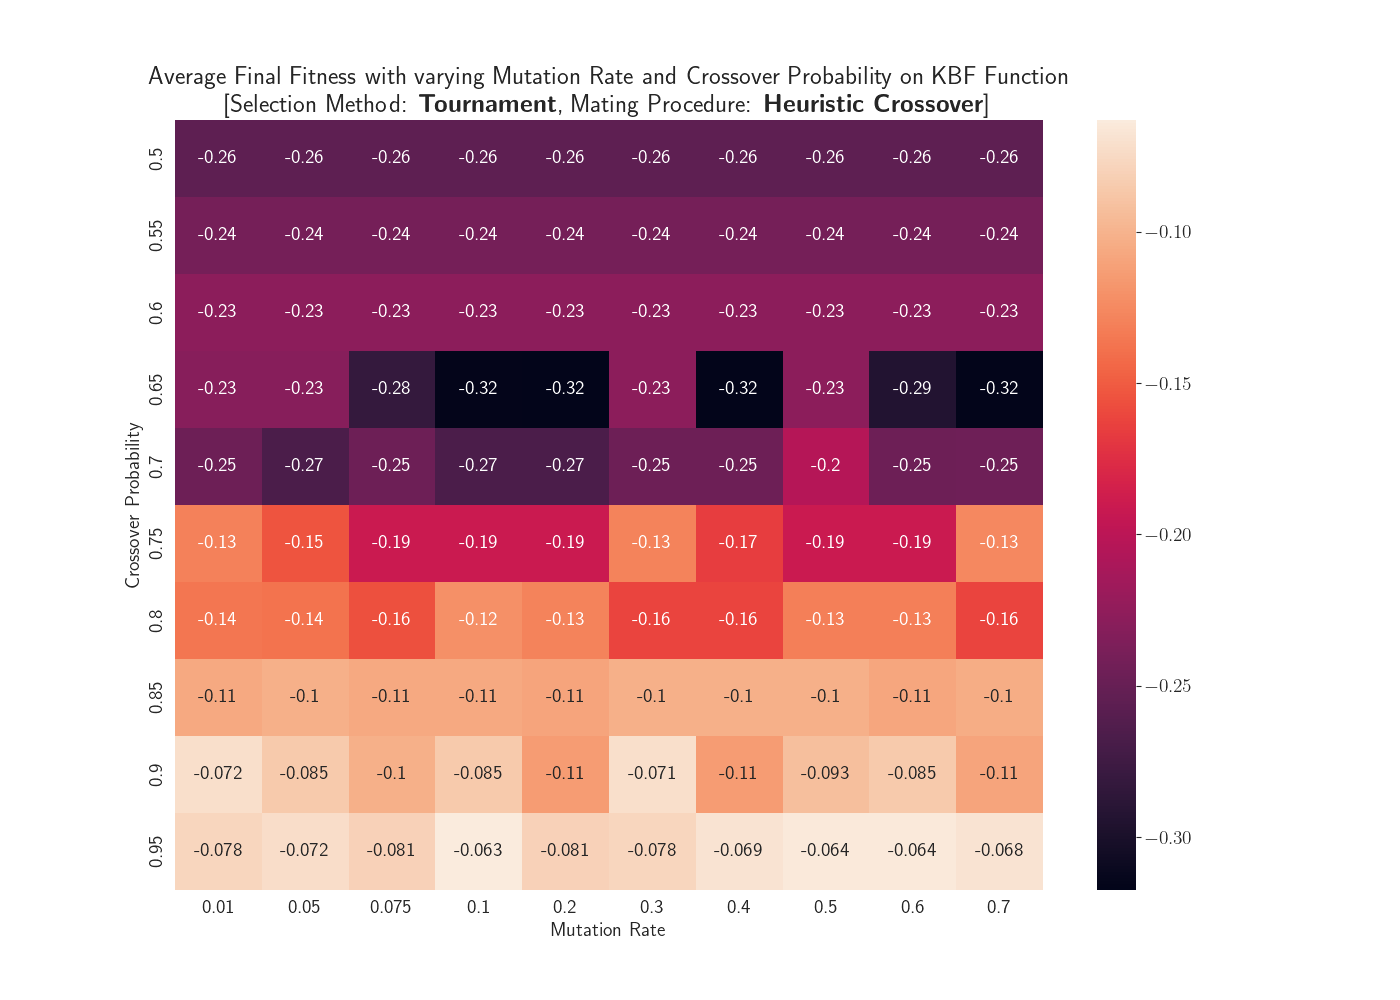
\includegraphics[width=\textwidth]{../figures/Permanent Images/AVGContour_Tournament_Heuristic Crossover.png}
        \caption{Average final fitness across entire population.}
        \label{fig:CGA_contour_tournament_Heuristic Crossover_AVG}
    \end{subfigure}
    \begin{subfigure}{0.48\textwidth}
        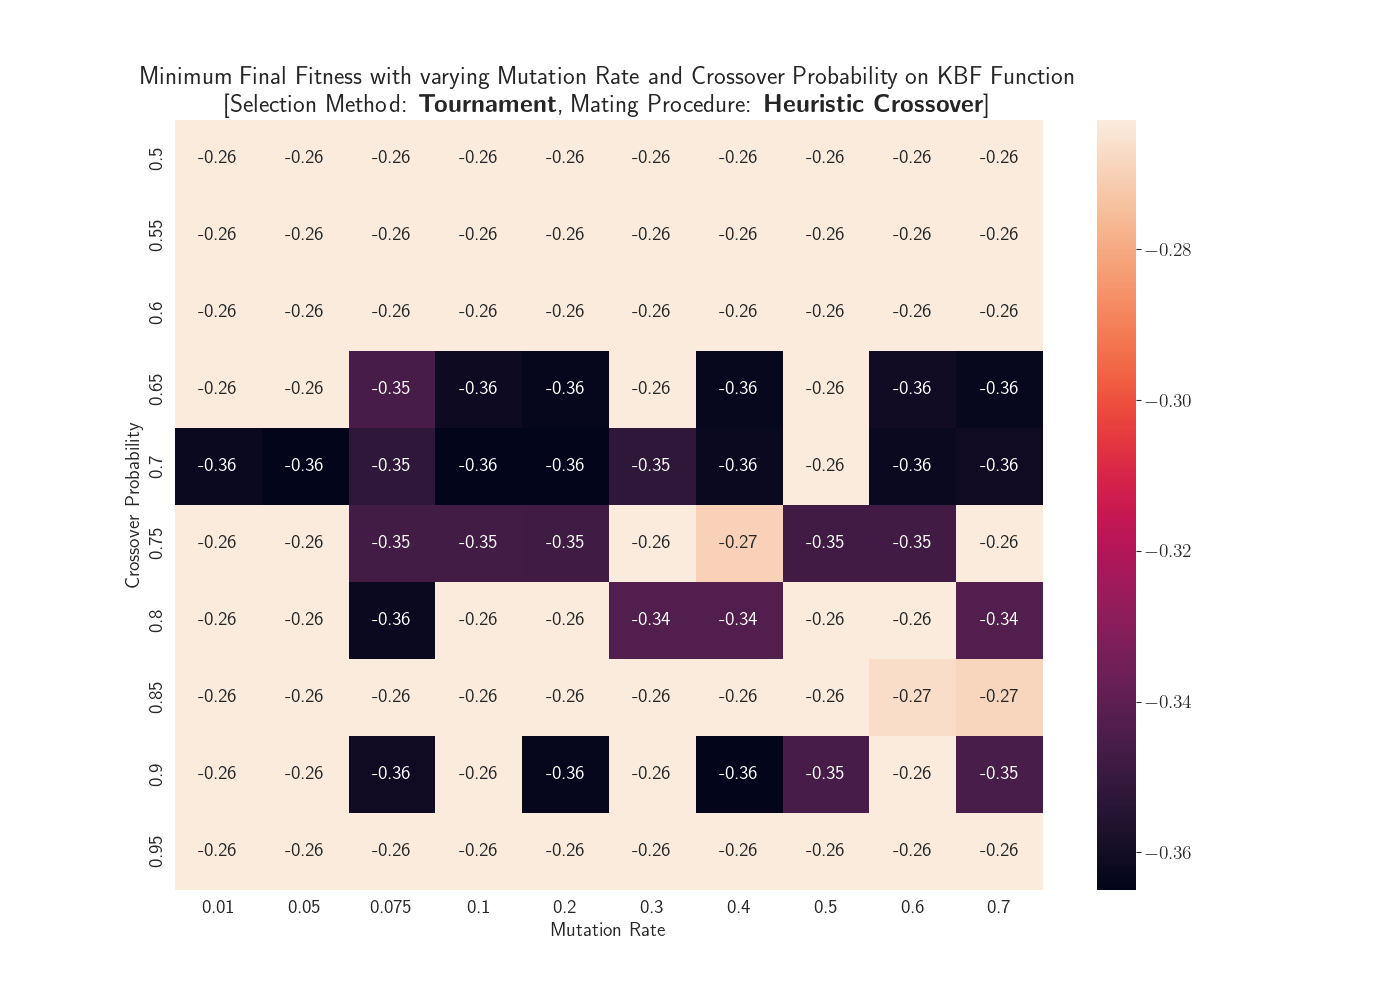
\includegraphics[width=\textwidth]{../figures/Permanent Images/MINContour_Tournament_Heuristic Crossover.png}
        \caption{Final (minimum) fitness of best individual.}
        \label{fig:CGA_contour_tournament_Heuristic Crossover_MIN}
    \end{subfigure}
    \captionsetup{justification=centering}
    \caption{Heat maps of the final fitness values after 100 iterations for the CGA using tournament selection and heuristic crossover. Here, the mutation rates and crossover probabilities were varied to assess their impact on performance.}
    \label{fig:CGA_contour_rates}
\end{figure}

Overall, a clear optimal set of hyperparameters emerges. Moving forward, the mutation rate is fixed at 0.1, and the crossover probability is set to 0.65. These values have proven to yield a consistently optimal performance for the algorithm, comfortably lying within the darker regions of the heat maps.

To reiterate and summarise this section of the report, the CGA is now constructed as follows:

\begin{itemize}
    \item \textbf{Selection Method:} Tournament Selection
    \item \textbf{Mutation Procedure:} Heuristic Crossover
    \item \textbf{Mutation Rate:} 0.1
    \item \textbf{Crossover Probability:} 0.65
    \item \textbf{Tournament Size:} 62
    \item \textbf{Number of Parents:} 62
    \item \textbf{Population Size:} 250
\end{itemize}

Fig. \ref{fig:CGA_fitness_evo_OPT} depicts the evolution of the fitness values over 100 iterations using the optimal hyperparameters delineated above. Note that the (minimum) fitness attributed to the best individual remains constant, because an individual within the population is stochastically initialised near the local maxima that the algorithm converges to. This is less likely to occur in the 8-dimensional comparison, where the minimum fitness is expected to evolve more noticeably,  given that the search space is significantly larger, and initialisation is handled with more care.

Fig. \ref{fig:optimal_convergence} depicts the convergence of the population to the second largest maxima over 4 and 80 iterations using the optimally-tuned CGA. Note that the horizontally and vertically distributed outliers are attributed to crossover. Regrettably, global maximum convergence remained elusive even after 100 iterations. However, there does seem to be a discernible trend of the algorithm converging towards the second-largest maxima in Fig. \ref{fig:optimal_convergence}, offering a promising indication of progress. 

The primary challenge lies in the fact that both the first and second largest maxima are situated along the non-linear constraint boundary of the optimisation problem, posing a difficult navigational challenge.
\vspace{-1mm}
\begin{figure}[H]
    \centering
    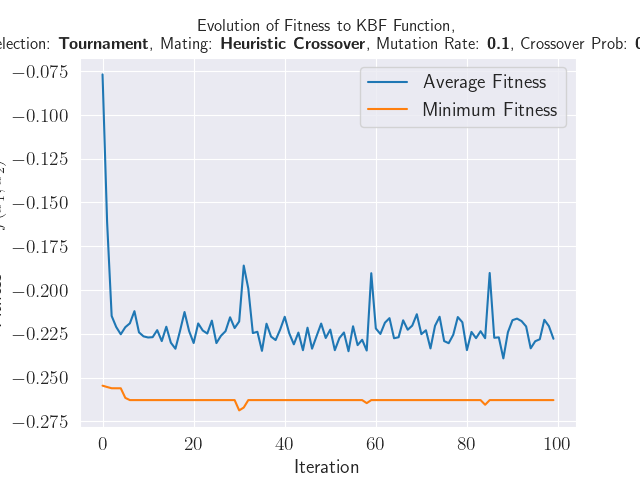
\includegraphics[width=0.45\textwidth]{../figures/Permanent Images/0.1_0.65_Fitness.png}
    \captionsetup{justification=centering}
    \caption{Evolution of the fitness values of the CGA population over 100 iterations for optimally-tuned CGA.}
    \label{fig:CGA_fitness_evo_OPT}
\end{figure}
\end{multicols}
\begin{figure}[H]
    \centering
    \begin{subfigure}{0.85\textwidth}
        \centering
        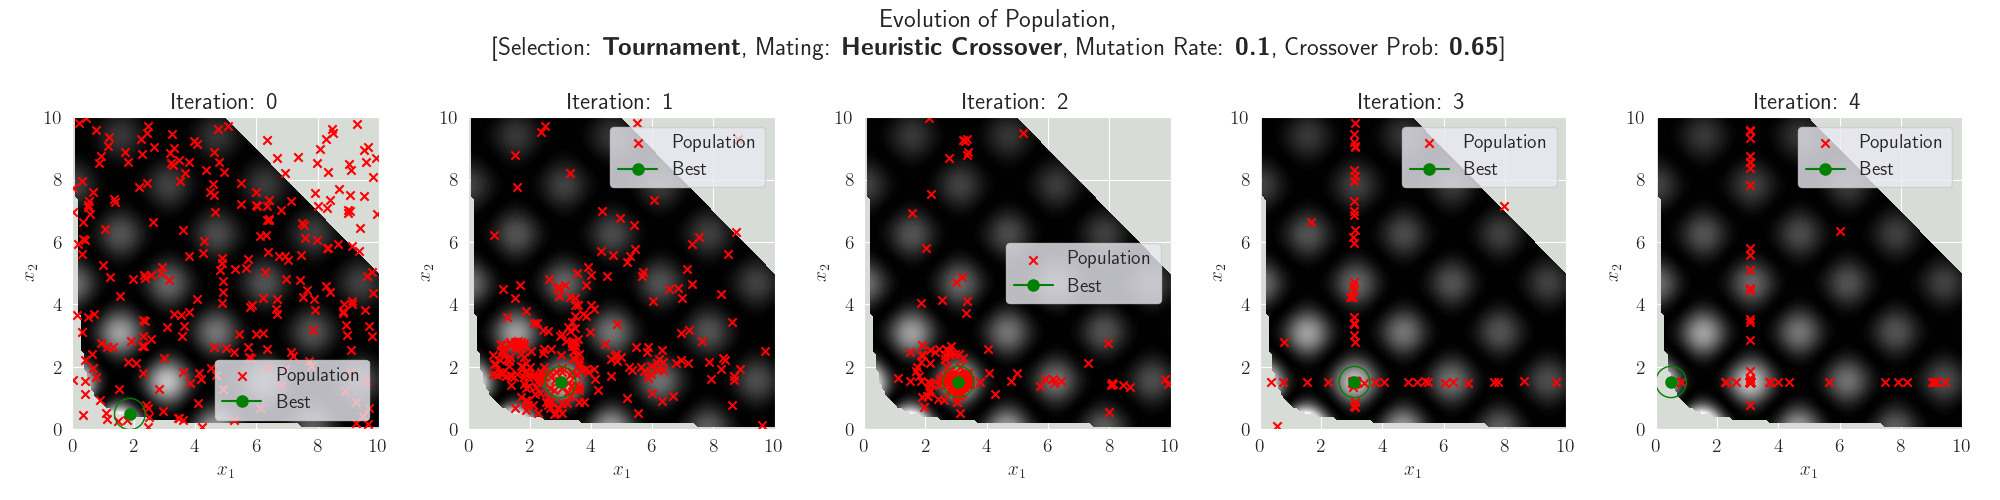
\includegraphics[width=\textwidth]{../figures/Permanent Images/0.1_0.65_Population.png}
        \caption{4 iterations.}
        \label{fig:optimal_5}
    \end{subfigure}
    \begin{subfigure}{\textwidth}
        \centering
        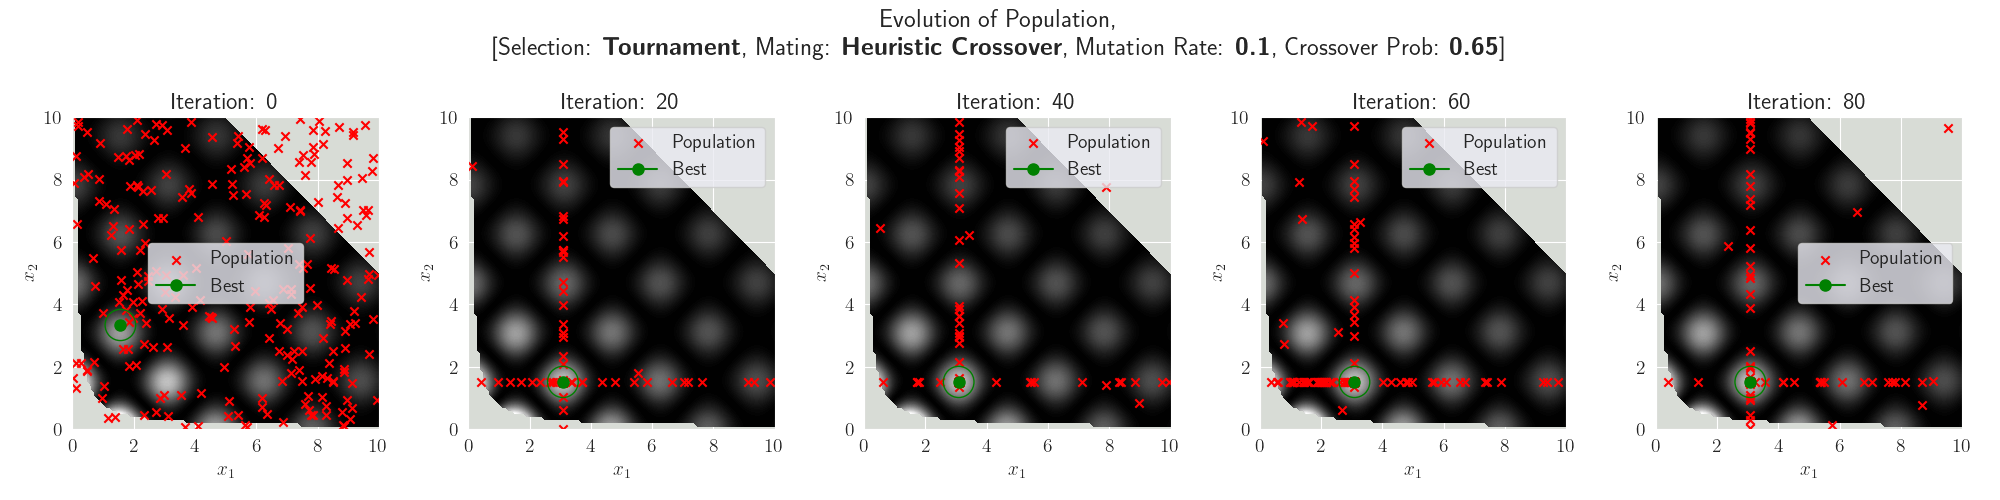
\includegraphics[width=0.85\textwidth]{../figures/Permanent Images/0.1_0.65_Population100.png}
        \caption{80 iterations.}
        \label{fig:optimat_100}
    \end{subfigure}
    \captionsetup{justification=centering}
    \caption{Evolution of the CGA population over 4 and 80 iterations using the optimal hyperparameters outlined at the end of Section \ref{sec:CGA_selection_mutation}. The second plot depicts the algorithm converging to a local maxima as a result of an individual being initialised near it.}
    \label{fig:optimal_convergence}
\end{figure}

\newpage

\begin{multicols}{2}
\section{Parallel Tempering (PT)}
\label{sec:PT}

Having obsererved the CGA's performance and its difficulty in identifying global maxima effectively, an informed decision was made to introduce Parallel Tempering (PT) as the second algorithm for comparison.

This is a Markvo Chain Monte Carlo (MCMC) optimisation approach presented in \cite{Earl_2005}. Similar to simulated annealing, (SA), it revolves around the idea of smoothening the search space by introducing a temperature parameter, $t$. 

By incorporating a Metropolis-Hasting acceptance probability that is proportional to $\exp(1/t)$, exploration of the solution space is encouraged at high temperatures, while exploitation of the local nature of the function is facilitated at low temperatures. At high temperatures, the acceptance distribution is is smoothened out by this proportionalilty, and the algorithm is then able to explore the search space more thoroughly. As the temperature diminishes, the acceptance distribution becomes more dependent on the fitness of the proposed solution to the KBF, enabling the algorithm to explore the local nature of the function.

However, PT incorporates the novel concept of Replica Exchange Monte Carlo. Unlike SA, which operates along a single tragectory, starting with a high temperature that gradually decreases, PT maintains multiple replicas of the system at different temperatures simultaneously. Each replica explores its own solution space, and exchanges of the solutions can occur between replicas at adjacent temperature levels. This exchange mechanism enhances global exploration by facilitating the movement of solutions between replicas operating at high and low temperature. 

This parallel exploration across temperatures improves the algorithm's ability to escape local optima, providing a valuable alternative to traditional single-trajectory methods like SA. Consequently, PT could emerge as a well-suited approach for maximising the highly multi-modal KBF.

Unfortunately, this introduces an elevated computational cost, due to the management of multiple replicas and the periodic exchange of solutions. However, the potential advantages in terms of global exploration of the KBF outweigh the added computational expense. This is especially true, considering the highly parallelisable nature of PT, which may allow for even more efficient utilisation of parallel computing resources than the CGA. 

\subsection{Implementation}

The discourse presented in \cite{Earl_2005} emphasises a delicate trade-off between optimising MCMC sampling outcomes and minimising computational efforts. Hence, the PT implementation presented here is deliberately crafted for flexibility, offering the ability to fine-tune the algorithm, as shown in Section \ref{sec:PTtuning}.

As per the guidance in \cite{parks2023geneticalgorithmsSA}, constraints are handled by simply rejecting any proposed changes that violate the constraints. This is accomplished within the Metropolis-Hastings criterion regarding the acceptance or rejection of a proposed change. This was determined as a suitable approach, given that the feasible space is non-disjoint, and the constraints are of the inequality type.

The approach can additionally be characterised as population-based, incorporating 10 replicas in accordance with the \textit{NUM\_REPLICAS} hyperparameter. Within each replica, there are 25 chains of solutions determined by the \textit{NUM\_CHAINS} hyperparameter. Consequently, the total number of solutions being evaluated at any given time is 250, which is equivalent to the population size of the CGA.

\subsubsection{Initialisation}
The chains are initialised within the range of 0 to 1, as advised by the guidance provided in \cite{NT90-A34350}, specifically under the SA-derived solution generation framework presented in Section \ref{sec:PT_update}.

This range persists throughout the algorithm, until function evaluations are necessitated, at which point the \textit{scale\_up} lambda function of listing \ref{PTpy} is called to return the solution in the original state space.

Mirroring the CGA implementation, solutions were initialised without consideration for their feasibility. Whilst initialising within the feasible solution space was observed to enhance performance, this approach was deliberately omitted to ensure fair comparisons between the PT and CGA. However, the performance was notably compromised, given that solutions initialised deep within the infeasible zones of the search space faced challenges in escaping under the Metropolis-Hastings acceptance criterion.

\subsubsection{Temperature Scheduling}

A significant source of flexibility in PT lies in setting and adapting the temperatures of the replicas, as discussed in \cite{Earl_2005}. Drawing insights from the previous work of \cite{CALDERHEAD20094028} on an unrelated, yet similar problem, this was taken advantage of by parameterising the temperature schedule between 0 and 1, as follows:

\begin{equation}
    T_i = \left(\frac{i}{{N_{\text{replicas}}}}\right)^p \quad \forall i \in \{1, \dots, N_{\text{replicas}}\}
    \label{eq:PTtemp}
\end{equation}

Here, $T_i$ denotes the temperature of the $i$th replica, and $N_{\text{replicas}}$ is the total number of replicas. The exponent $p$ is a hyperparameter referred to as \textit{POWER\_TERM} that can be tuned to optimise the performance of the algorithm. 

Fig. \ref{fig:PTtemp} illustrates the influence of parameter $p$ on the temperature schedule. It intuitively demonstrates how $p$ affects the balance between exploration and exploitation. A higher value of $p$ corresponds to a slower and more gradual increase in temperature, promoting a conducive environment for exploration. A smaller value of $p$ results in a more rapid increase in temperature, encouraging exploitation of the local nature of the function.

\begin{figure}[H]
    \centering
    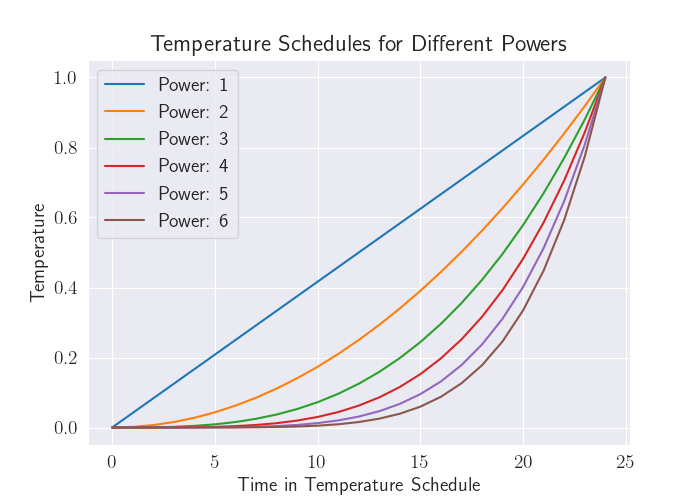
\includegraphics[width=0.48\textwidth]{../figures/Permanent Images/Power_Progression.png}
    \captionsetup{justification=centering}
    \caption{Temperature schedule (\ref{eq:PTtemp}) for the PT algorithm for different values of the \textit{POWER\_TERM} hyperparameter.}
    \label{fig:PTtemp}
\end{figure}

Tuning this balance is crucial for the algorithm's performance against the KBF, and is conducted in Section \ref{sec:PTtuning}. While alternative approaches, such as geometric progression \cite{Earl_2005} are recommended in most literature, the above formulation was made to enhance control over the replica temperatures.

\subsubsection{Replica Exchange}

The most popular approach to replica exchange, as outlined in \cite{Earl_2005}, involves periodic execution. The interchange of solutions between replicas at adjacent temperature levels occurs at regular intervals. In this implementation, periodic exchange is guided by the hyperparameter \textit{EXCHANGE\_PARAM}. This hyperparameter assumes values in the range of 0 to 1, representing the proportion of total iterations that must pass before another swap takes place. A value of 0.05 indicates that a swap occurs every 5 iterations when the maximum number of iterations is set to 100.

However, a second approach has also been implemented, which will be referred to as stochastic exchange. In this configuration, the possibility of replica exchange exists in every iteration, and the hyperparameter \textit{EXCHANGE\_PARAM} now functions as the probability governing the occurrence of this swap. 

Both have been introduced to enhance the flexibilty of the algorithm, allowing for either a more deterministic or stochastic approach to replica exchange. The optimal choice is determined in Section \ref{sec:PTtuning}.

Upon meeting the conditions for a swap, the replicas are sequentially traversed in ascending order of temperature. Each replica undergoes an attempt to exchange all of its solutions with the subsequent replica in the sequence. The likelihood of accepting such a swap is dictated by the adapted Metropolis-Hastings acceptance criterion, as detailed in Section \ref{sec:PT_MA}.

\subsubsection{Metropolis Update}
\label{sec:PT_update}

The inspiration for proposing a new solution stems from \cite{NT90-A34350}, which introduces a routine that leverages accumulated experience from prior iterations to generate SA update steps. Given the similarity between SA and PT, this approach was deemed suitable for the PT implementation.

In particular, a new solution is generated by:
\begin{equation}
\mathbf{x}_{\text{new}} = \mathbf{x}_{\text{old}} + \mathbf{D}\mathbf{u}
\label{eq:PTupdate}
\end{equation}
In this context, $\mathbf{u}$ represents a vector of uniformly distributed random numbers within the range of $[-1, 1]$, while $\mathbf{D}$ is a diagonal matrix specifying the maximum permissible step size in each dimension of the state space. In this PT implementation, $\mathbf{D}$ is uniquely defined for each solution across all replicas. Following the acceptance of a new solution, the matrix $\mathbf{D}$ is updated using the formula:
\[
\mathbf{D}_{\text{new}} = (1-\alpha)\mathbf{D}_{\text{old}} + \alpha \omega \mathbf{R}
\]
Here, the constants $\alpha$ and $\omega$ are set at 0.1 and 2.1 respectively, in accordance with the guidlines presented in \cite{NT90-A34350}. The matrix $\mathbf{R}$ is a diagonal matrix whose elements represent the magnitudes of the successful changes made to each dimension within a specific solution.

\subsubsection{Metropolis-Hastings Acceptance Criterion}
\label{sec:PT_MA}

The probability of accepting a proposed solution is determined by the Metropolis-Hastings acceptance criterion. This has been specifically formulated to work alongside the "adapting" update step, (\ref{eq:PTupdate}), with additional insights drawn from the works of \cite{NT90-A34350} and \cite{Neal_1996}. The probability of accepting a new solution generated by Eq. (\ref{eq:PTupdate}) is given by:
\[
    \hspace{-2mm}P_{\text{accept}} = \min\left[1, \exp\left(\frac{f(\mathbf{x_{\text{new}}}) - f(\mathbf{x_{\text{old}}})}{k \cdot T_i \cdot \tilde{d}}\right)\right]
\]
In the above formulation, the negation of the objective function: $-f(\mathbf{x})$, represents the fitness of a solution $\mathbf{x}$, $k$ is the Boltzmann constant, $T_i$ is the temperature of the $i$th replica, and $\tilde{d}$ is euclidean normed distance between the old and new solutions.

However, when judging the swap of two solutions through a replica exchange, the acceptance probability is instead adapted to:
\[
    \hspace{-2mm}P_{\text{accept}} = \min\left[1, \exp\left(\frac{f(\mathbf{x_{\text{new}}}) - f(\mathbf{x_{\text{old}}})}{k \tilde{d}} \left(\frac{1}{T_{\text{old}}} - \frac{1}{T_{\text{new}}}\right)\right)\right]
\]
in accordance with \cite{Neal_1996}. This imposes a harsher standard for the acceptance of a swap between replicas operating at vastly different temperatures, which is a desirable feature, especially when the power term, $p$, is set to a high value.

\subsubsection{Termination}

Again, the algorithm terminates after a maximum number of iterations, (defined as a hyperparameter), in this section of the study. A more stringent convergence criterion is adopted for the comparison between the two algorithms in Section \ref{sec:CGA_QEG_comparison}. The solution with the lowest fitness value across all replicas is then returned as the optimal solution to the optimisation problem.

The total number of iterations is fixed at 100, which generally proved insufficient for the algorithm to achieve complete convergence. Rather than emphasising complete convergence, the assessment centers around tracking the evolution of average fitness values. This approach provides insights into the algorithm's effectiveness and speed, gauging its progress within the limited span of 100 iterations.

\subsection{Tuning the PT}
\label{sec:PTtuning}

As with Section \ref{sec:CGA_selection_mutation}, the flexibility offered by PT was first explored using the parallelised experiments presented in listing \ref{PT_TuningExperimentspy}.

Unlike the CGA table, (Table \ref{tab:CGAexploration}), the preliminary exploratory findings presented for PT, (Table \ref{tab:exchange_results}), imply a subtle correlation between the power term of the temperature schedule and the algorithm's performance. Final fitness values exhibit relative constancy, hinting at no potential connection. However, the variability in algorithm performance appears more pronounced when considering the approach to replica exchange.

\begin{figure}[H]
    \centering
    \begin{subfigure}{0.48\textwidth}
        \centering
        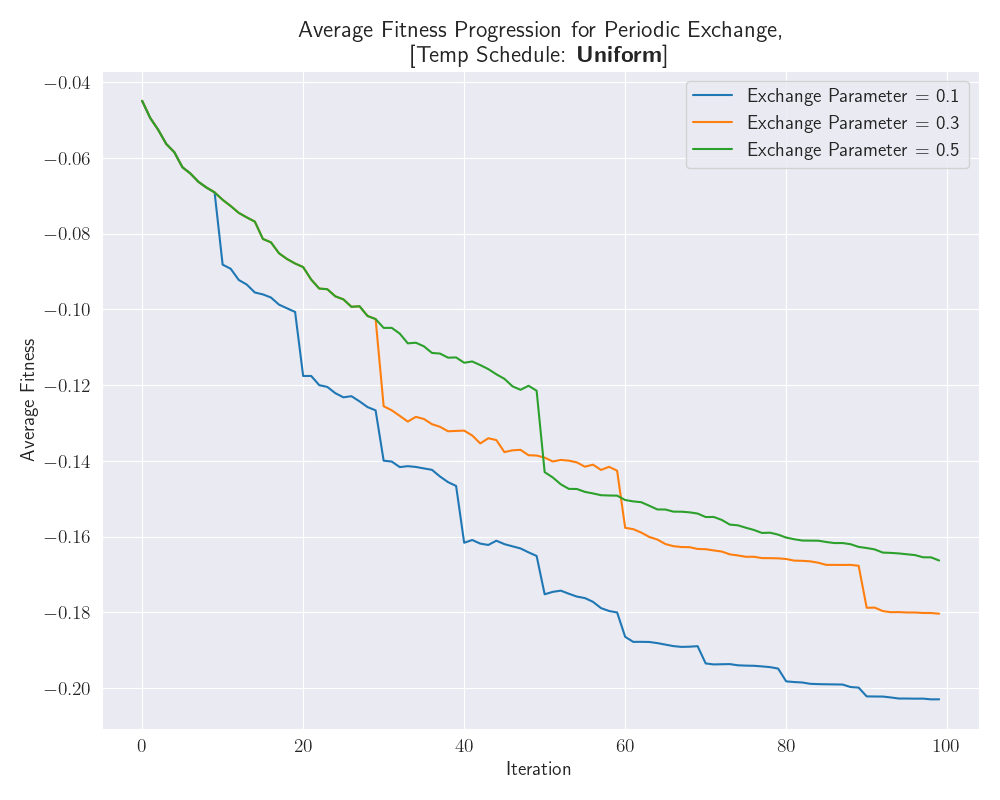
\includegraphics[width=\textwidth]{../figures/Permanent Images/PT_Avg_Fitness_Evolution.png}
        \caption{Periodic Exchange}
        \label{fig:periodic_fitness}
    \end{subfigure}
    \begin{subfigure}{0.48\textwidth}
        \centering
        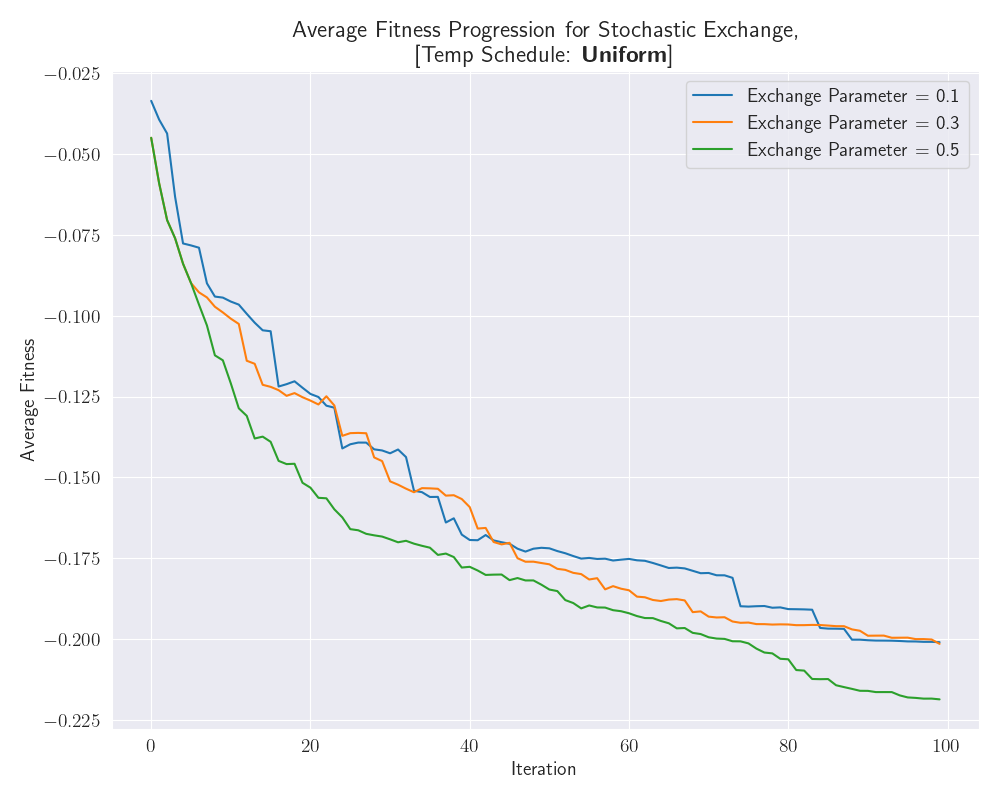
\includegraphics[width=\textwidth]{../figures/Permanent Images/PT_Avg_Fitness_Evolution_stoch.png}
        \caption{Stochastic Exchange}
        \label{fig:stochastic_fitness}
    \end{subfigure}
    \captionsetup{justification=centering}
    \caption{Evolution of average fitness values of the PT solutions over 100 iterations for the two approaches to replica exchange. Temperature scheduling was kept uniform.}
    \label{fig:fitness_PT}
\end{figure}

Fig. \ref {fig:fitness_PT} instead illustrates the evolution of the average fitness values across all 100 iterations for both exchange procedures. The result present a clear distinction between the two approaches that remains consistent with repitition. 

The periodic exchange approach seems to exhibit a higher dependency on the value assigned to the exchange parameter. In contrast, the stochastic exchange approach appears to follow a consistent descent, irrespective of the exchange parameter value. This observation is unexpected, considering that the exchange parameter is anticipated to exert a similarly significant influence on both approaches. In both cases, the exchange parameter affects the frequency of swaps, which is expected to impact the algorithm's ability to escape local optima.

Additionally, the descent depicted in Fig. \ref{fig:periodic_fitness} seems steeper when the exchange parameter assumes smaller values. This aligns with expectations, as a smaller exchange parameter corresponds to a higher frequency of swaps in the periodic case. Here, the exchange parameter is interpreted as the proportion of total iterations that transpire before another swap takes place. When applied to the KBF, PT demonstrates greater efficacy when the algorithm is permitted to exchange solutions more frequently. This implies that increased exploration of the search space is well-suited to optimising the KBF.

Figures \ref{fig:heatmap_periodic} and \ref{fig:heatmap_stochastic} present a final analysis of these hyperparameters. However, the stochastic heatmap, \ref{fig:min_stochastic_heatmap}, did not exhibit any consistency or superiority over the periodic heatmap, \ref{fig:min_periodic_heatmap}, leading to no further consideration of stochastic exchange, given its suboptimal and unpredictable behavior.

In contrast, a consistent pattern unveiled itself in Fig. \ref{fig:min_periodic_heatmap}, which persisted across repetitions. The PT algorithm, when applied to the KBF, consistently demonstrated a inclination towards a lower exchange parameter paired with a low power term. This may be rationalised by the fact that a lower exchange parameter corresponds to a heightened frequency of swaps, facilitating dialogue between the replicas and encouraging more exploration. Conversely, a low power term fosters a delicate equilibrium between exploration and exploitation, as evident in Fig. \ref{fig:PTtemp}. The preference for uniform temperature scheduling likely stems from its enhanced capability to focus on local changes, after arriving at a particular optimum. Any exploratory capabilities stem from replica exchange, after which the algorithm can then focus on exploiting the local nature of the function.

Overall, these results imply that optimal settings for the PT algorithm on the KBF involve a power term of 1 and an exchange parameter of 0.01. These values are associated with a uniform temperature schedule and replica exchange taking place at every iteration. They position the PT algorithm favorably within the lighter regions of Fig. \ref{fig:min_periodic_heatmap}.

\columnbreak

In summary and to reiterate, the PT algorithm is now constructed as follows:

\begin{itemize}
    \item \textbf{Number of Replicas:} 10
    \item \textbf{Number of Chains:} 25
    \item \textbf{Power Term:} 1
    \item \textbf{Exchange Procedure:} Always
    \item \textbf{Exchange Parameter:} N/A
\end{itemize}

Fig. \ref{fig:PToptimal_fitness} depicts the evolution of the fitness values over 100 iterations using the optimal hyperparameters delineated above. The fitness of the best solution drops noticeably once better solutions are identified and arrived at through the MCMC updating process, however the progress is much slower than that of the CGA.

\begin{figure}[H]
    \centering
    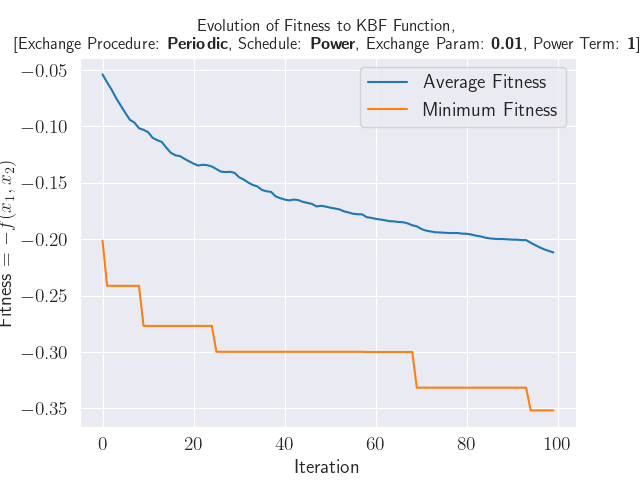
\includegraphics[width=0.48\textwidth]{../figures/Permanent Images/0.01_1_Periodic_Fitness.png}
    \captionsetup{justification=centering}
    \caption{Evolution of the fitness values of the optimally-tuned PT solutions over 100 iterations.}
    \label{fig:PToptimal_fitness}
\end{figure}

The top row in Fig. \ref{fig:PToptimal_evo} depicts the iterative evolution of the solutions. Notably, all solutions consistently converge towards the prominent maxima, and the global maximum is successfully identified in every repetition. The PT algorithm has demonstrated superior capabilities in exploration compared to the CGA.

The optimal solution is denoted by a green circle. For a more insightful comprehension of the Markov Chain Monte Carlo (MCMC) updating process, a particular solution within the final replica is emphasised in yellow. This solution is monitored throughout all iterations and it seems to become ensnared in a local optimum during the earlier iterations. However, it then successfully breaks free through the exchange mechanism and begines to converge towards a larger maximum in subsequent iterations.

The bottom row in Fig. \ref{fig:PToptimal_evo} showcases the final solutions of each replica, organised by temperature and superimposed over the temperature-smoothed KBF contours. The arrangement follows an ascending temperature order, with the replica at the lowest temperature positioned on the left. These results shed light on the fundamental dynamics of the algorithm.

At lower temperatures, all solutions exhibit a clear inclination toward the higher, global maxima of the KBF. This preference arises from ample exploration of the search space. In contrast, solutions at higher temperatures display a more dispersed distribution, converging around local optima. 

Additionally, although these higher temperatures encourage localised exploration, the replica exchange mechanism facilitates the movement of solutions within the final temperature towards the larger maximas. Subsequent iterations are anticipated to drive convergence of solutions at higher temperatures towards the global maxima as well.
\end{multicols}

\begin{multicols}{2}
\begin{figure}[H]
    \centering
    \begin{subfigure}{0.48\textwidth}
        \centering
        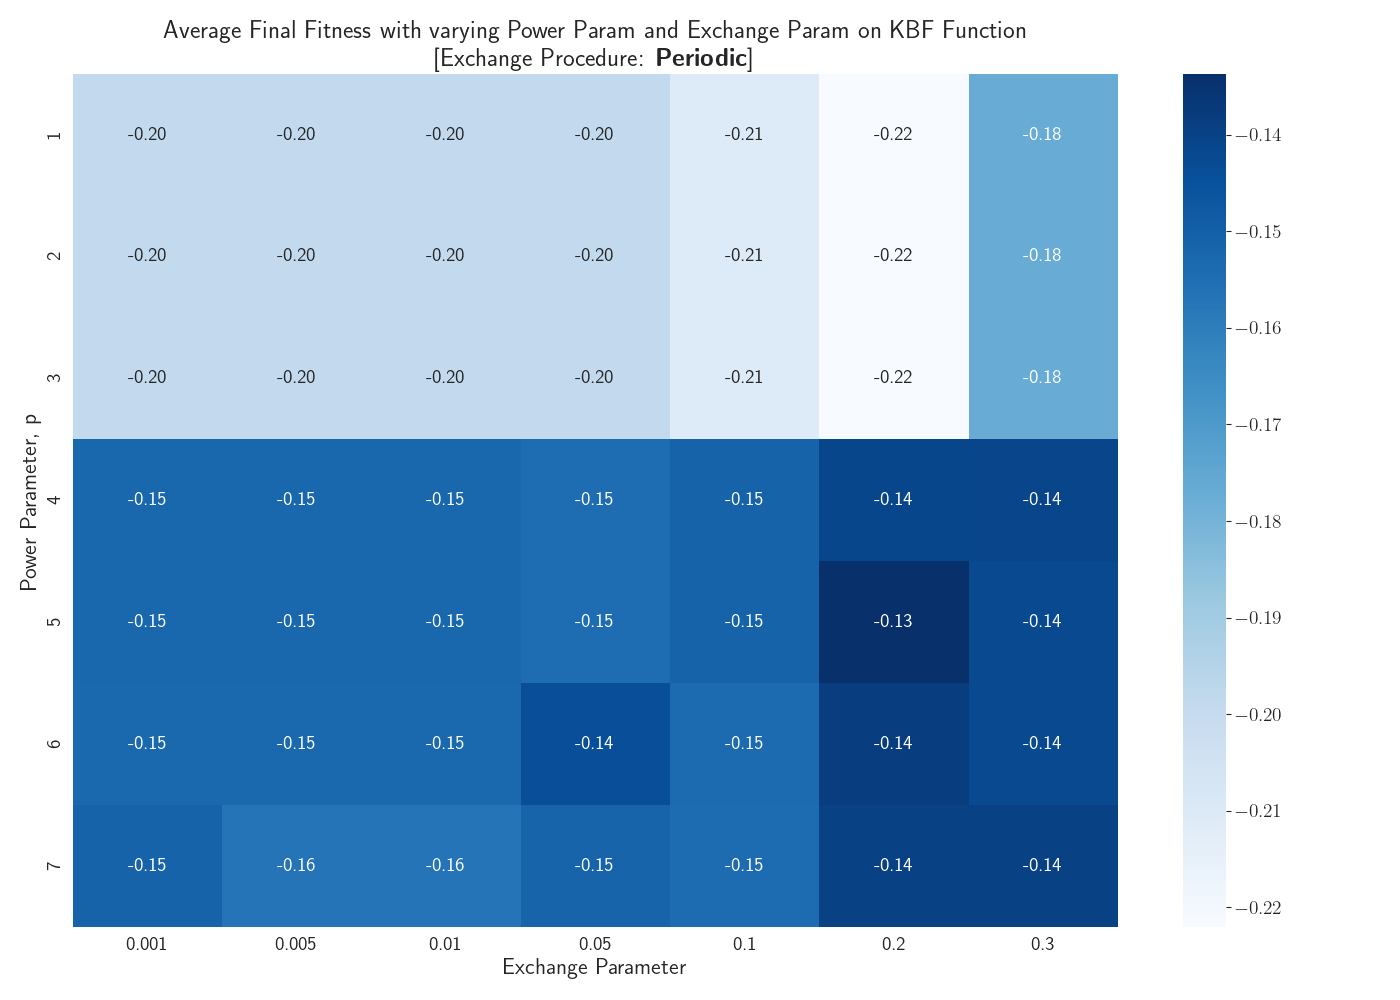
\includegraphics[width=\textwidth]{../figures/Permanent Images/PT_Avg_Fitness_Heatmap_Periodic.png}
        \caption{Average Fitness Values}
        \label{fig:avg_periodic_heatmap}
    \end{subfigure}
    \begin{subfigure}{0.48\textwidth}
        \centering
        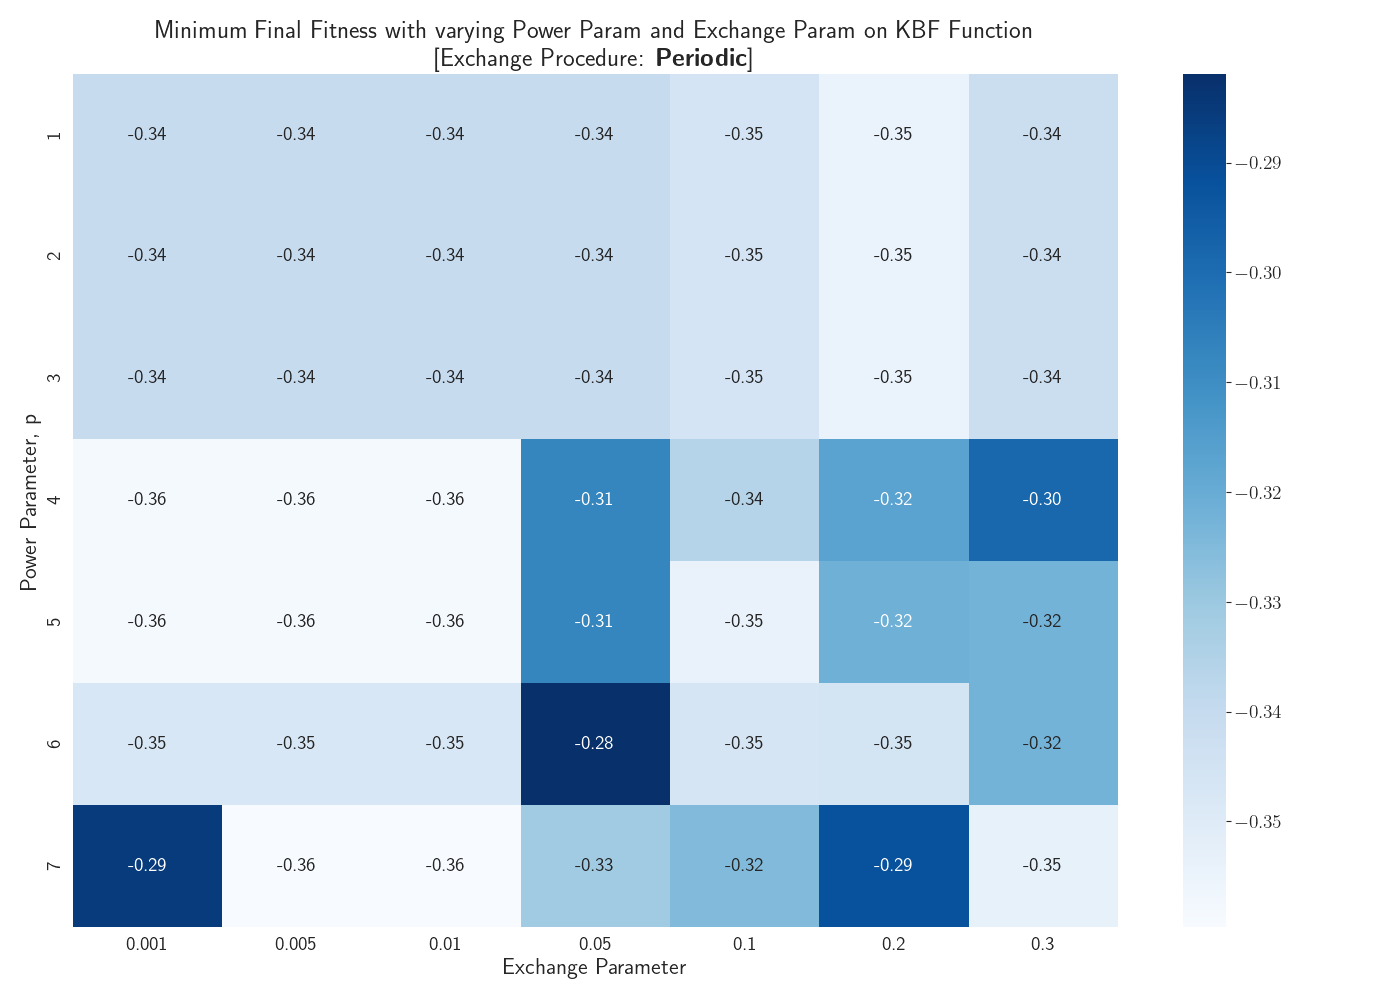
\includegraphics[width=\textwidth]{../figures/Permanent Images/PT_Min_Fitness_Heatmap_Periodic.png}
        \caption{Minimum Fitness Values}
        \label{fig:min_periodic_heatmap}
    \end{subfigure}
    \captionsetup{justification=centering}
    \caption{Heatmaps of the final fitness values after 100 iterations for the PT algorithm using periodic exchange. Here, the power term and exchange parameter were varied to assess their impact on performance. Despite the somewhat varied outcomes between repitition, a consistent trend emerges - the PT algorithm demonstrates a preference for a lower exchange parameter coupled with a moderate power term.}
    \label{fig:heatmap_periodic}
\end{figure}

\begin{figure}[H]
    \centering
    \begin{subfigure}{0.48\textwidth}
        \centering
        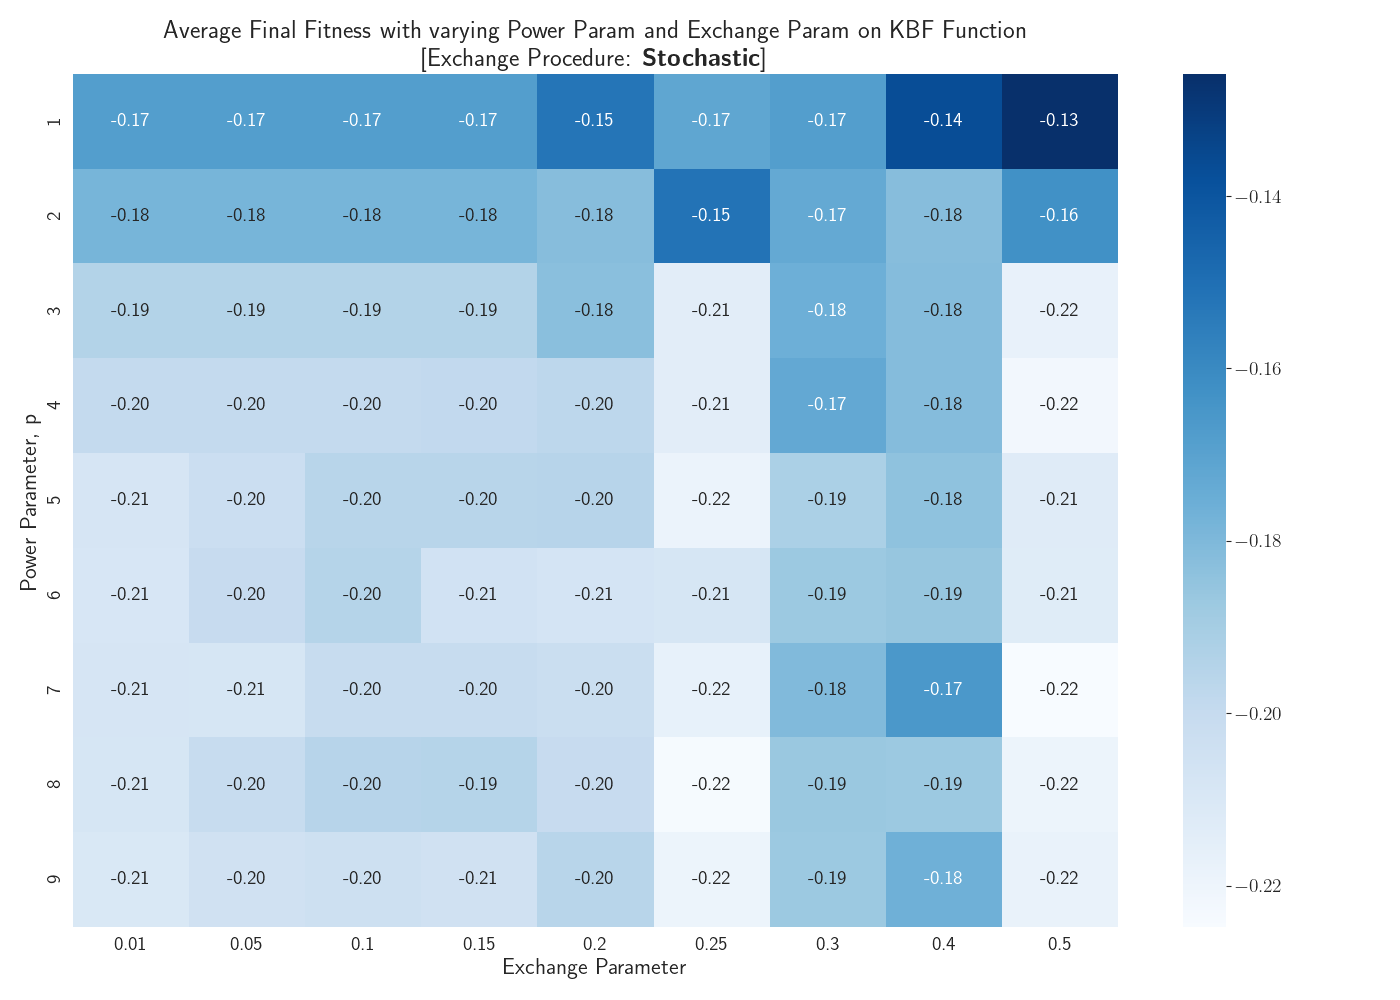
\includegraphics[width=\textwidth]{../figures/Permanent Images/PT_Avg_Fitness_Heatmap_Stochastic.png}
        \caption{Average Fitness Values}
        \label{fig:avg_stochastic_heatmap}
    \end{subfigure}
    \begin{subfigure}{0.48\textwidth}
        \centering
        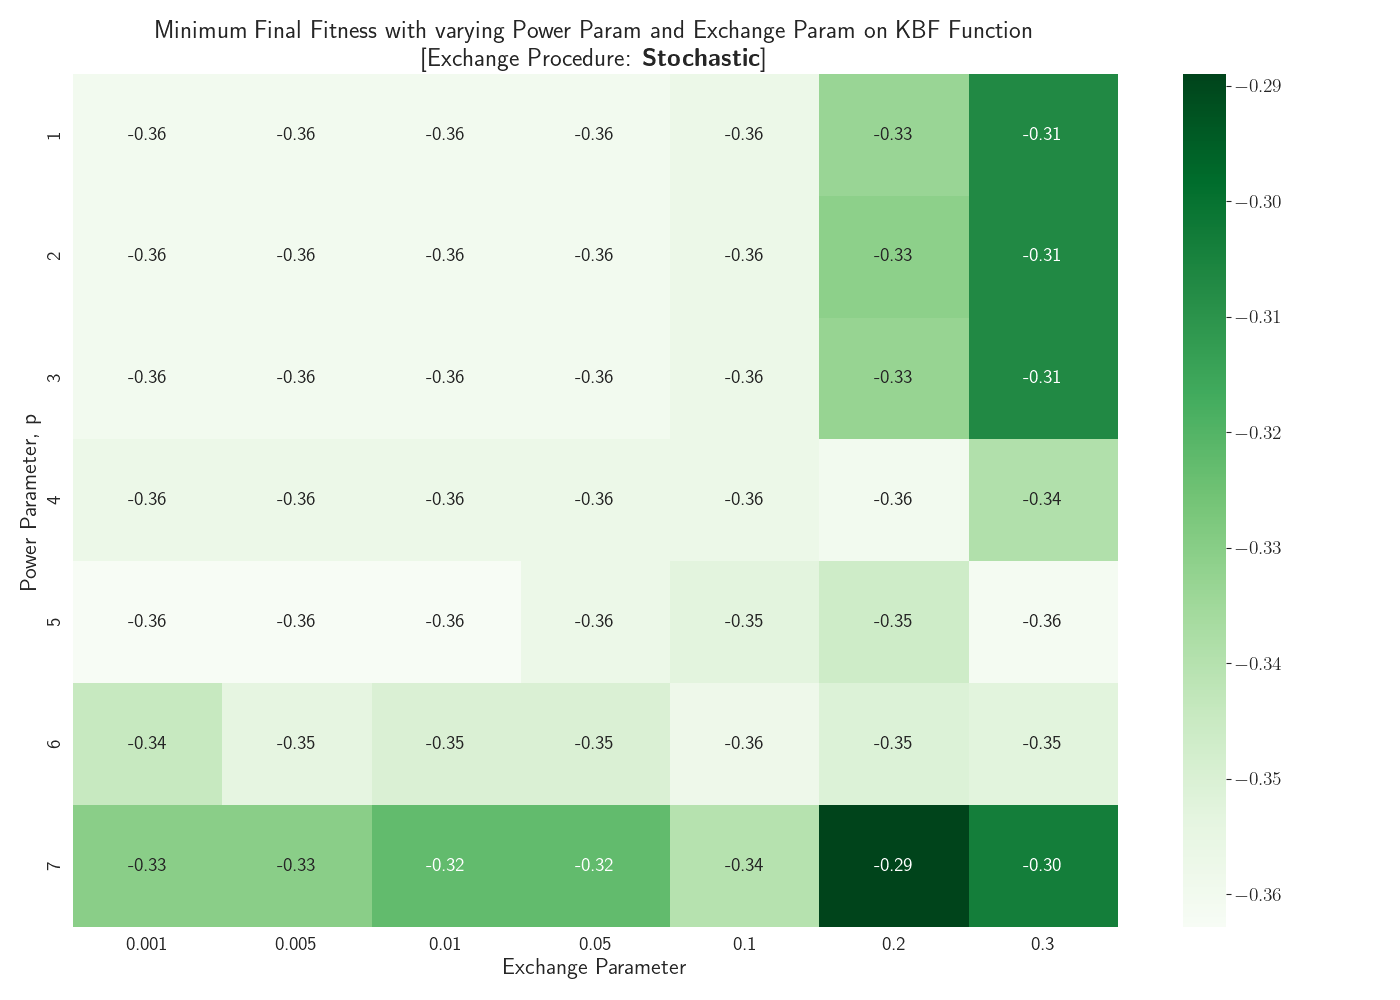
\includegraphics[width=\textwidth]{../figures/Permanent Images/PT_Min_Fitness_Heatmap_Stochastic.png}
        \caption{Minimum Fitness Values}
        \label{fig:min_stochastic_heatmap}
    \end{subfigure}
    \captionsetup{justification=centering}
    \caption{Heatmaps of the final fitness values after 100 iterations for the PT algorithm using stochastic exchange. Here, the power term and exchange parameter were varied to assess their impact on performance. The values for the best (minimum) final fitness varied greatly upon repitition. Generally, performance was outmatched by periodic exchange, which was also more consistent and controllable.}
    \label{fig:heatmap_stochastic}
\end{figure}
\end{multicols}

\begin{figure}[H]
    \centering
    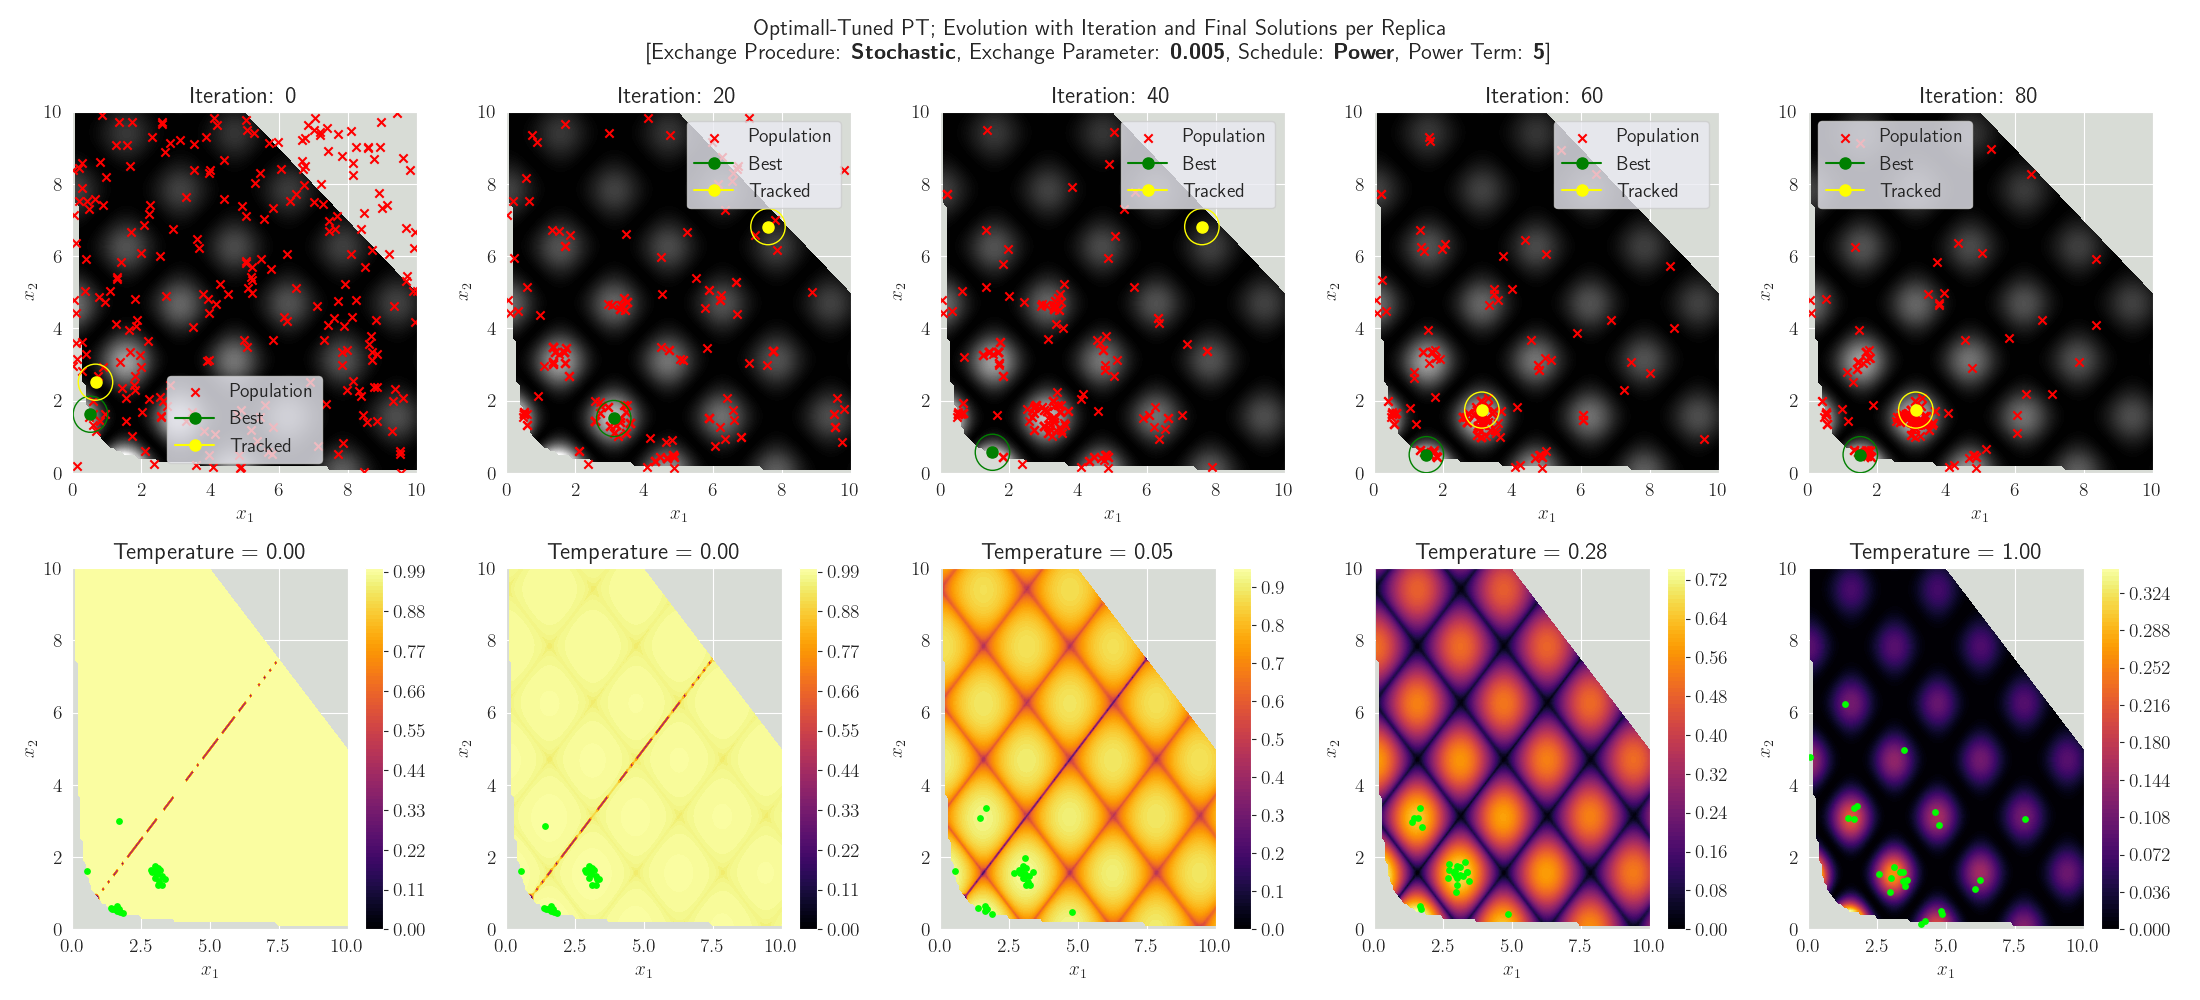
\includegraphics[width=1\textwidth]{../figures/Permanent Images/PT_Optimal_Tuning.png}
    \captionsetup{justification=centering}
    \caption{Visualisation of the optimally-tuned PT algorithm. The first row illustrates its evolution with each iteration. The optimal solution is marked with a green circle. To enhance the understanding of the MCMC updating process, a specific solution within the final replica is highlighted in yellow. The second row displays the final solutions arranged for each replica, overlaid across the smoothened KBF, $f(\mathbf{x})^T$, to help visualise the theory of PT. Lower temperatures facilitate exploration, while higher temperatures encourage exploitation. However, exchange ensures that solutions at higher temperatures are also driven towards the global maxima.}
    \label{fig:PToptimal_evo}
\end{figure}

\begin{multicols}{2}
\section{Comparison}
\label{sec:CGA_QEG_comparison}

After fine-tuning both algorithms for the 2-dimensional KBF, a comparative analysis was conducted to assess their performances in optimising the 8-dimensional KBF using the code presented in listing \ref{FinalComparisonpy}. 50 optimisation loops were conducted for each algorithm, each with a different initialisation.  Collected data included expected values and standard deviations of fitness values, as well as the mean CPU time taken to complete all 10,000 iterations and the average iteration count at which convergence occurred.

To uphold fairness and reproducibility, these initialisations were shared between both algorithms. They were generated using random number seeds within the \textit{generate\_initial} function, which is part of the \textit{helper\_functions.py} file \ref{helper_functionspy}. The implementation of this function was crucial for ensuring reproducible outcomes and guaranteeing that solutions were initialised away from the global maxima. This was achieved by imposing a constraint that the maximum function value of these initial collections never exceeded 0.3.

Each run was limited to a maximum of 10,000 function evaluations, and convergence was identified as the point where the $l_2$-normed difference between the minimum fitness values of consecutive iterations stayed within a tolerance of 0.00025 for 1300 consecutive iterations. This was deemed appropriate after the trial run outlined in Section \ref{sec:trial}, in which the convergence points of both algorithms were correclty identified under this criterion.

\subsection{Trial Run}
\label{sec:trial}

Prior to the experiment, a trial run of 15,000 funcation evaluations was conducted using one initialisation to assess the suitability of the convergence criterion, and to set expectations.

The outcomes are detailed in Table \ref{tab:trial_comparison} and illustrated in Fig. \ref{fig:trial_fitness}. These findings underscore a particularly noteworthy result.

The two algorithms yielded fairly divergent solutions, as described in the last row of Table \ref{tab:trial_comparison}. The CGA underwent significant change within the initial 1\% of iterations, after which it stabilised near its ultimate solution. In contrast, the PT algorithm consistently evolved over the entire span of 15,000 iterations. Consequently, the CGA demonstrated superior performance in the early iterations, but the PT algorithm ultimately surpassed it by converging to a lower minimum fitness value. This observation is a promising indication of the PT's capacity to escape local optima and explore the search space more efficiently.

However, this advantage comes with a trade-off in terms of increased computational demands. Specifically, the PT algorithm required approximately double the time to finish the 15,000 iterations compared to the CGA. Additionally, the PT algorithm required an extra 2551 iterations to converge to its optimal solution, resulting in a greater time investment of approximately 335.9 seconds, with respect to the CGA.

While the CGA required less implementation effort, it consistently exhibited swift convergence, quickly reaching solutions in close proximity to its optimal outcome. In contrast, the PT algorithm displayed a gradual descent, highlighting its greater exploratory nature. 

Upon repeated trials, the PT algorithm was unable to consistently overtake the CGA within 10,000 iterations. As a result, it is unlikely that this dynamic will be evident in the final comparison. Nevertheless, the trial run yields valuable insights into the relative performance of the two algorithms and sheds light on potential trade-offs. Additionally, it reinforces the appropriateness of the convergence criterion, which was subsequently employed in the final comparative analysis.

Although the PT algorithm's final solutions were only marginally superior to those of the CGA, it demanded significantly more CPU time to attain this outcome. Depending on the application and the consistency of this result, the CGA might be a more preferable algorithm. This observation is a valuable insight from the trial run, and emphasises the importance of considering expectations and identifying standard deviations in the final comparison.

An additional notable observation is the pronounced and turbulent trajectory in the average fitness values of the CGA after convergence, as depicted in Figure \ref{fig:trial_fitness}. This phenomenon can be ascribed to the inherent stochasticity of crossover, leading to a consistent dispersion of the population across regions of the function characterised by low values. In contrast, the average fitness of the PT algorithms exhibits a gradual descent, attributed to the greater determinism of its update procedure under the Metropolis-Hastings acceptance criterion.

\begin{table}[H]
    \centering
    \begin{tabular}{|c|c|c|}
    \hline
    \textbf{Metric} & \textbf{CGA} & \textbf{PT} \\
    \hline
    \textbf{Final Avg. Fitness} & -0.4971 & -0.4646 \\
    \hline
    \textbf{Final Min. Fitness} & -0.6901 & -0.7081 \\
    \hline
    \textbf{Total Time Taken} & 299.2 & 592.7 \\
    \hline
    \textbf{Iters to Convergence} & 9349 & 11990 \\
    \hline
    \textbf{Optimal Solutions} & $\begin{bmatrix} 3.104 \\ 3.027 \\ 1.624 \\ 0.5872 \\ 0.5363 \\ 0.6130 \\ 0.5294 \\ 0.4808 \end{bmatrix}$ & $\begin{bmatrix} 3.111 \\ 2.948 \\ 3.071 \\ 1.643 \\ 0.3356 \\ 0.4636 \\ 0.4284 \\ 0.2457 \end{bmatrix}$ \\
    \hline
    \end{tabular}
    \captionsetup{justification=centering}
    \caption{Trial comparison between CGA and PT, after 15,000 iterations with one shared initialisation, (random seed = 538405).}
    \label{tab:trial_comparison}
\end{table}

\begin{figure}[H]
    \centering
    \begin{subfigure}{0.48\textwidth}
        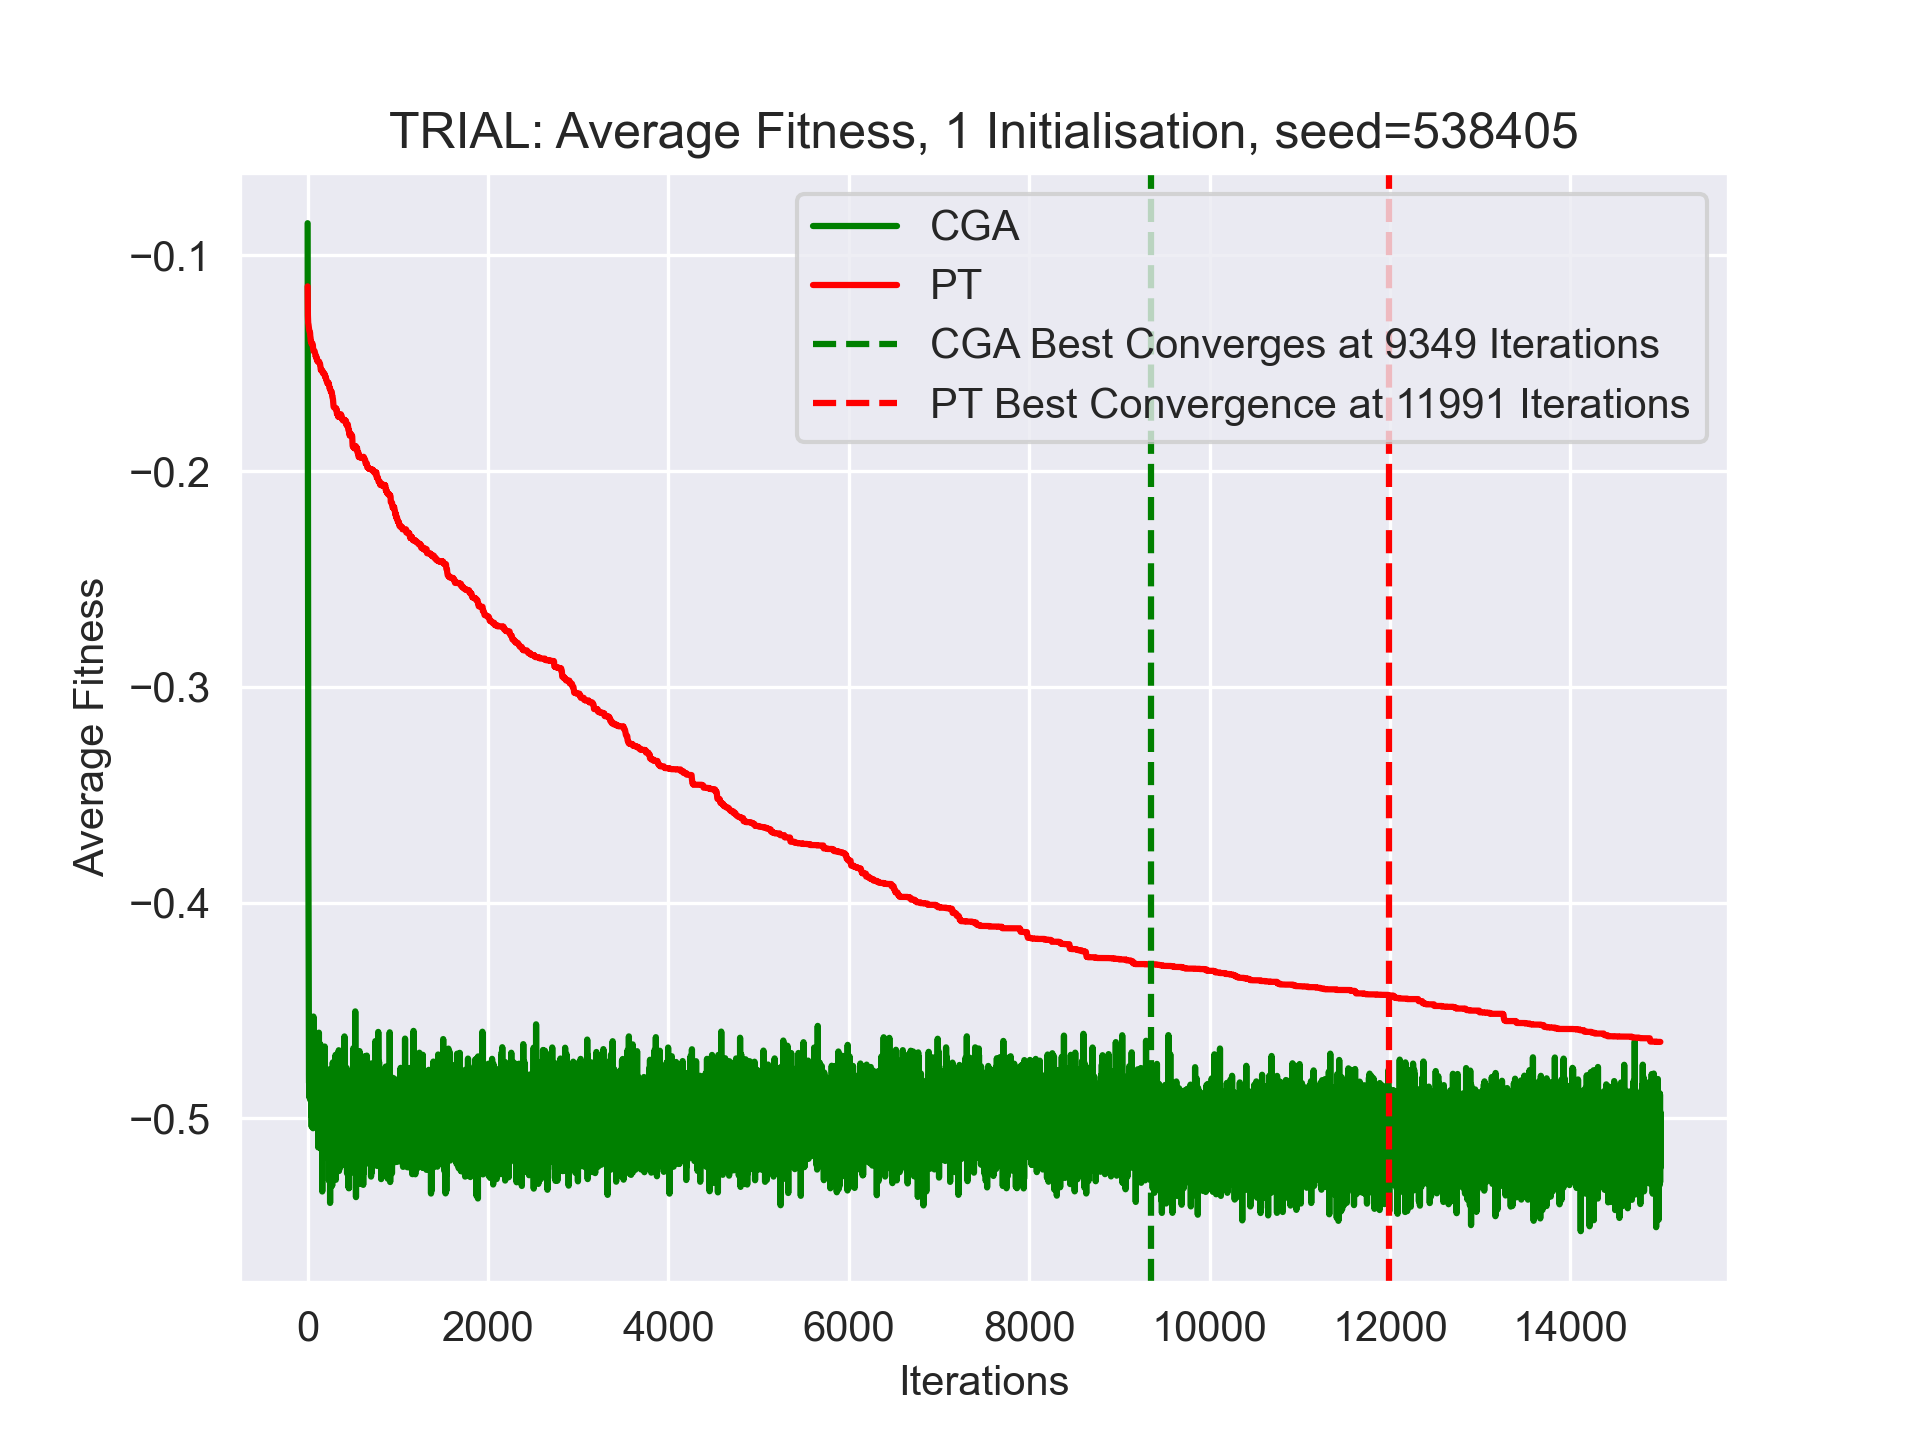
\includegraphics[width=\textwidth]{../figures/Final Comparison/CGA vs PT Average Fitness TRIAL.png}
        \caption{Average fitnesses.}
        \label{fig:AVG_trial_fitness}
    \end{subfigure}
    \begin{subfigure}{0.48\textwidth}
        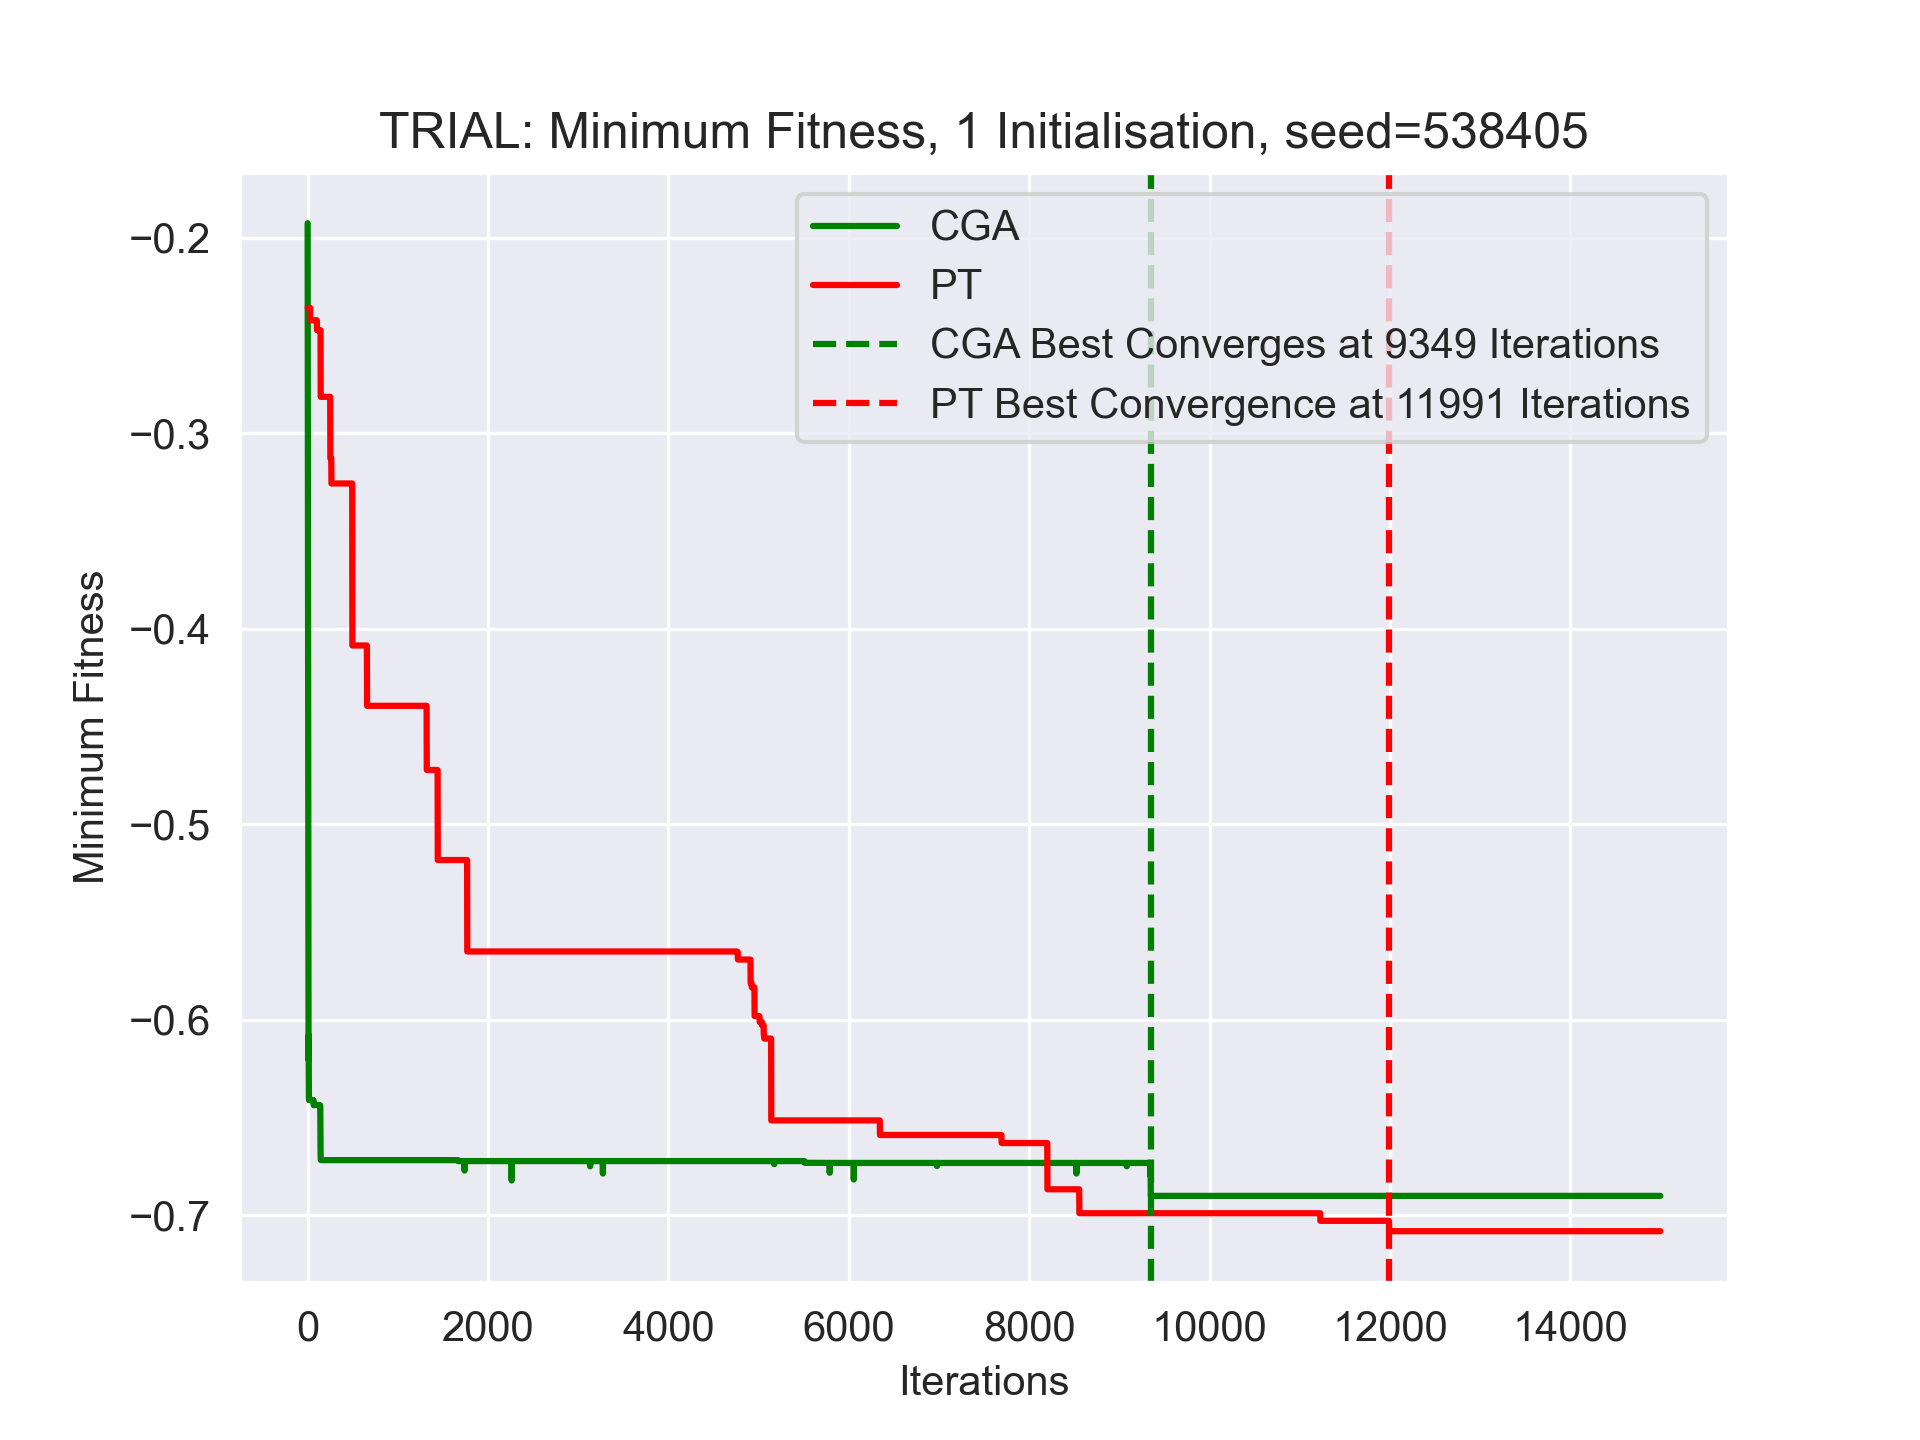
\includegraphics[width=\textwidth]{../figures/Final Comparison/CGA vs PT Minimum Fitness TRIAL.png}
        \caption{Minimum fitnesses.}
        \label{fig:MIN_trial_fitness}
    \end{subfigure}
\captionsetup{justification=centering}
\caption{Evolution of fitness values over 15,000 iterations for the CGA and PT algorithms, using a single initialisation as a trial run, (random seed = 538405).}
\label{fig:trial_fitness}
\end{figure}

\subsection{Final Comparison}
Having validated the experiment with a trial run, the final comparison was conducted using 50 different intialisations, generated with the following random seeds:

[588541, 776379, 146310, 178897, 630385, 455226, 75798, 763473, 295412, 733068, 521014, 926074, 667371, 58738, 543141, 263789, 572073, 46141, 360713, 247094, 379228, 395478, 102912, 110855, 602020, 673151, 903361, 138526, 750056, 969814, 998683, 433667, 885222, 414036, 401547, 862285, 671914, 26963, 764090, 99348, 794953, 642883, 292349, 168953, 736085, 528540, 558369, 41243, 168530, 285025]

The results are presented in Table \ref{tab:final_comparison} and Fig. \ref{fig:final_fitness}. 

\begin{table}[H]
    \centering\hspace{-2mm}
    \begin{tabular}{|c|c|c|}
    \hline
    \textbf{Metric} & \textbf{CGA} & \textbf{PT} \\
    \hline
    \textbf{Expected Final Avg. Fitness} & -0.5431 & -0.4181 \\
    \textbf{Std. in Final Avg. Fitness} & 0.01658 & 0.01536 \\
    \hline
    \cellcolor{lightgray}\textbf{Expected Final Min. Fitness} &\cellcolor{lightgray} -0.7099 &\cellcolor{lightgray} -0.6913 \\
    \cellcolor{lightgray}\textbf{Std. in Final Min. Fitness} &\cellcolor{lightgray} 0.02083 &\cellcolor{lightgray} 0.03044 \\
    \hline
    \textbf{Expected Total Time Taken} & 90.48 & 170.2 \\
    \textbf{Std. in Time Taken} & 1.412 & 4.544 \\
    \hline
    \cellcolor{lightgray}\textbf{Mean Iters to Convergence} &\cellcolor{lightgray} 4915 &\cellcolor{lightgray} 5247 \\
    %\textbf{Mean Best Solution} & "[3.09591858 3.03587839 2.74237 1.38674504 0.69373476 0.42972398 0.35063415 0.35390884]" & "[3.11472988 2.96313606 2.76836915 1.3707924 0.65082983 0.50910921 0.40659709 0.40242741]" \\
    \hline
    \end{tabular}
    \captionsetup{justification=centering}
    \caption{Final comparison between CGA and PT, after 10,000 iterations with 50 shared initialisations.}
    \label{tab:final_comparison}
\end{table}

\begin{figure}[H]
    \centering
    \begin{subfigure}{0.48\textwidth}
        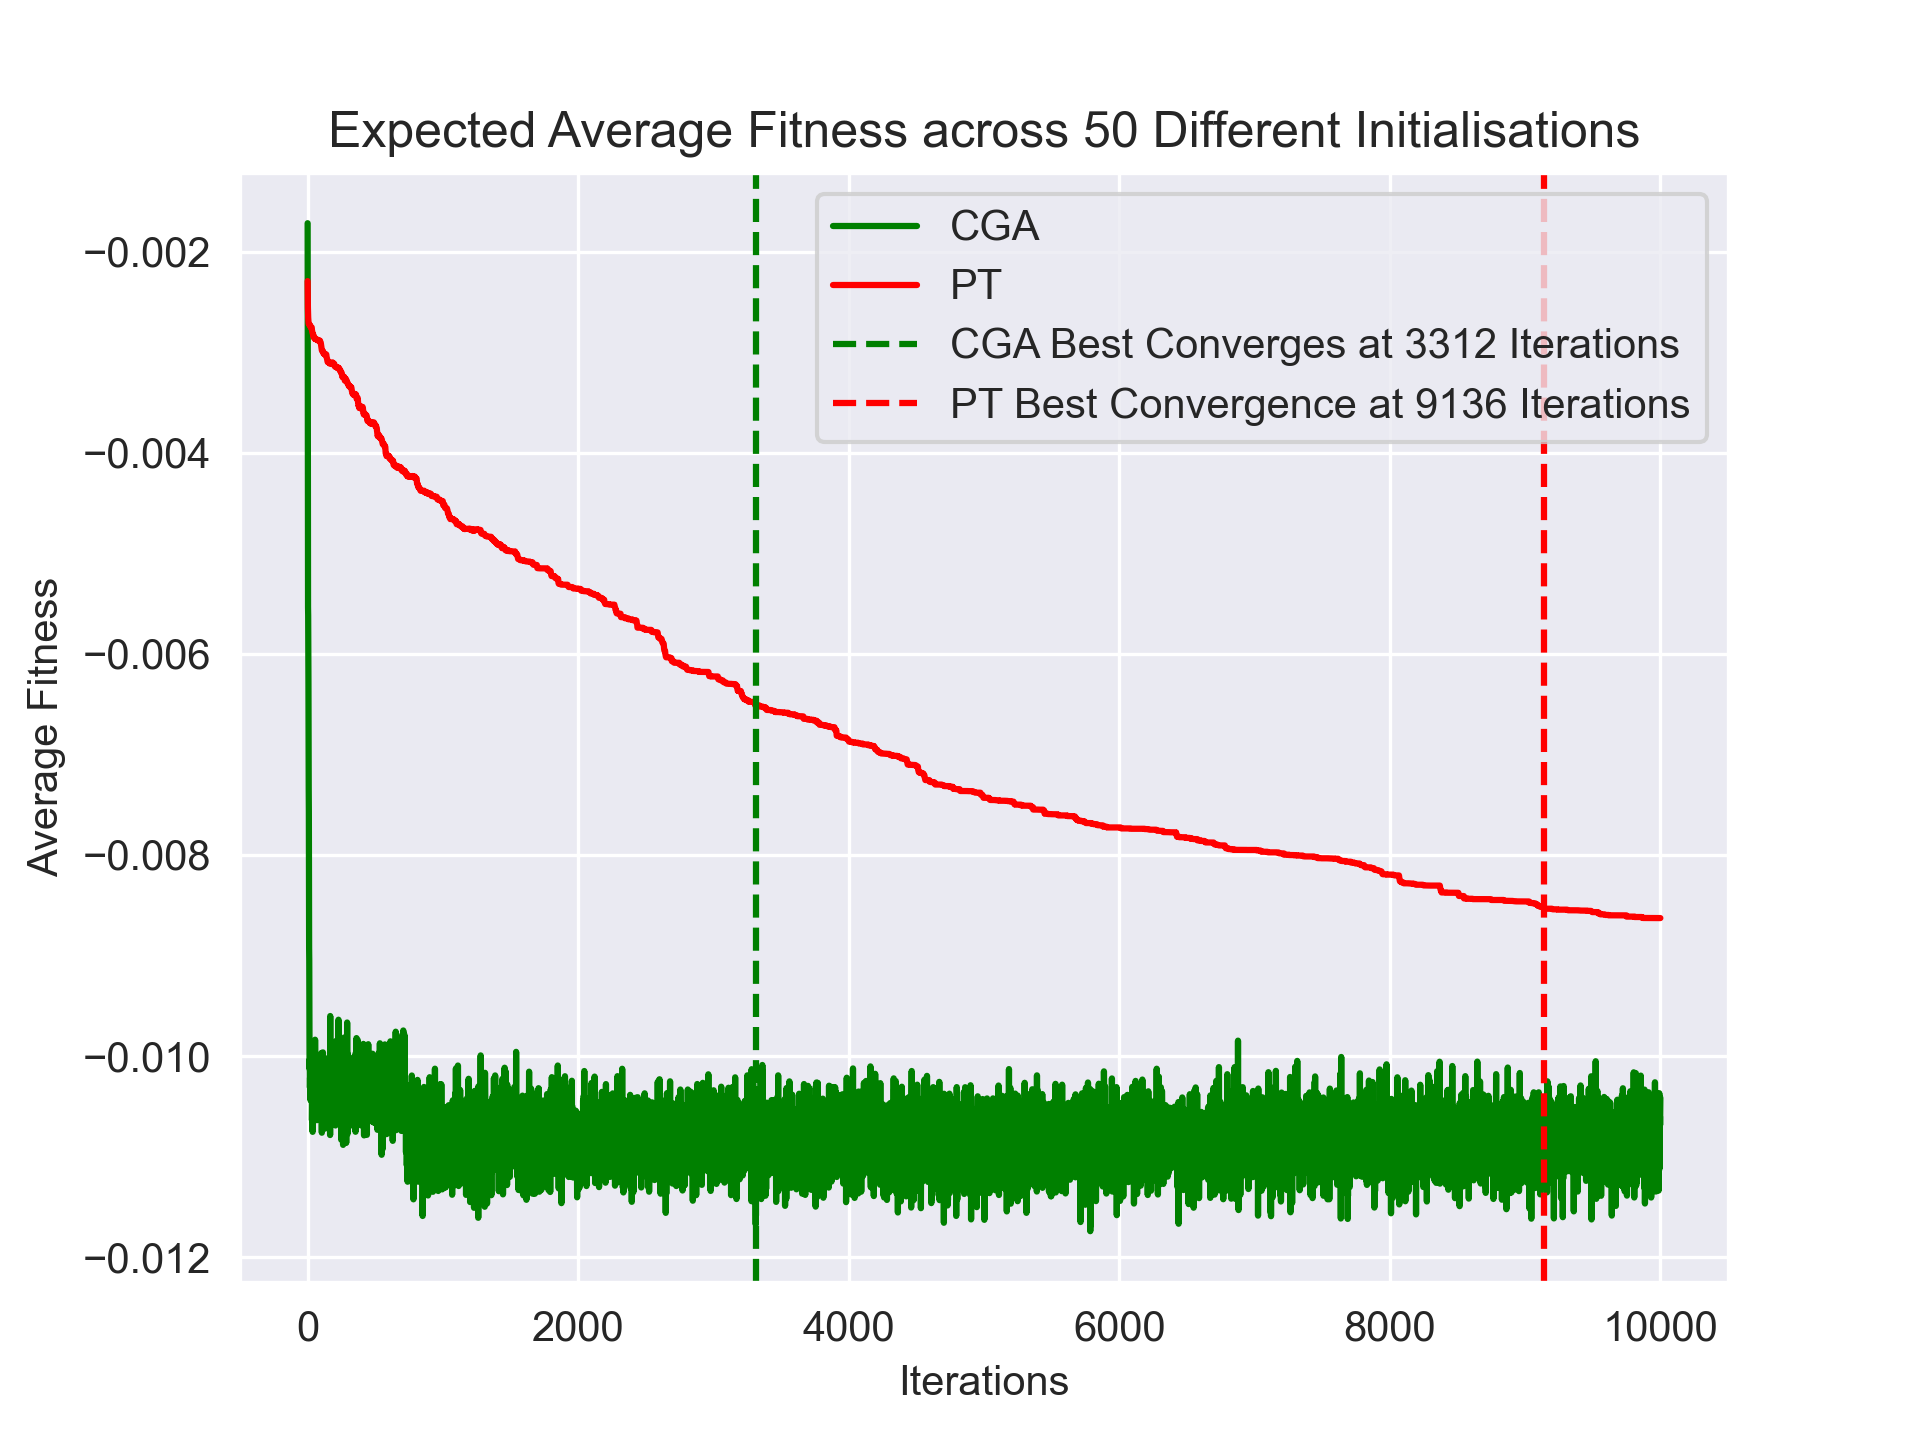
\includegraphics[width=\textwidth]{../figures/Final Comparison/CGA vs PT Average Fitness.png}
        \caption{Average fitnesses.}
        \label{fig:AVG_final_fitness}
    \end{subfigure}
    \begin{subfigure}{0.48\textwidth}
        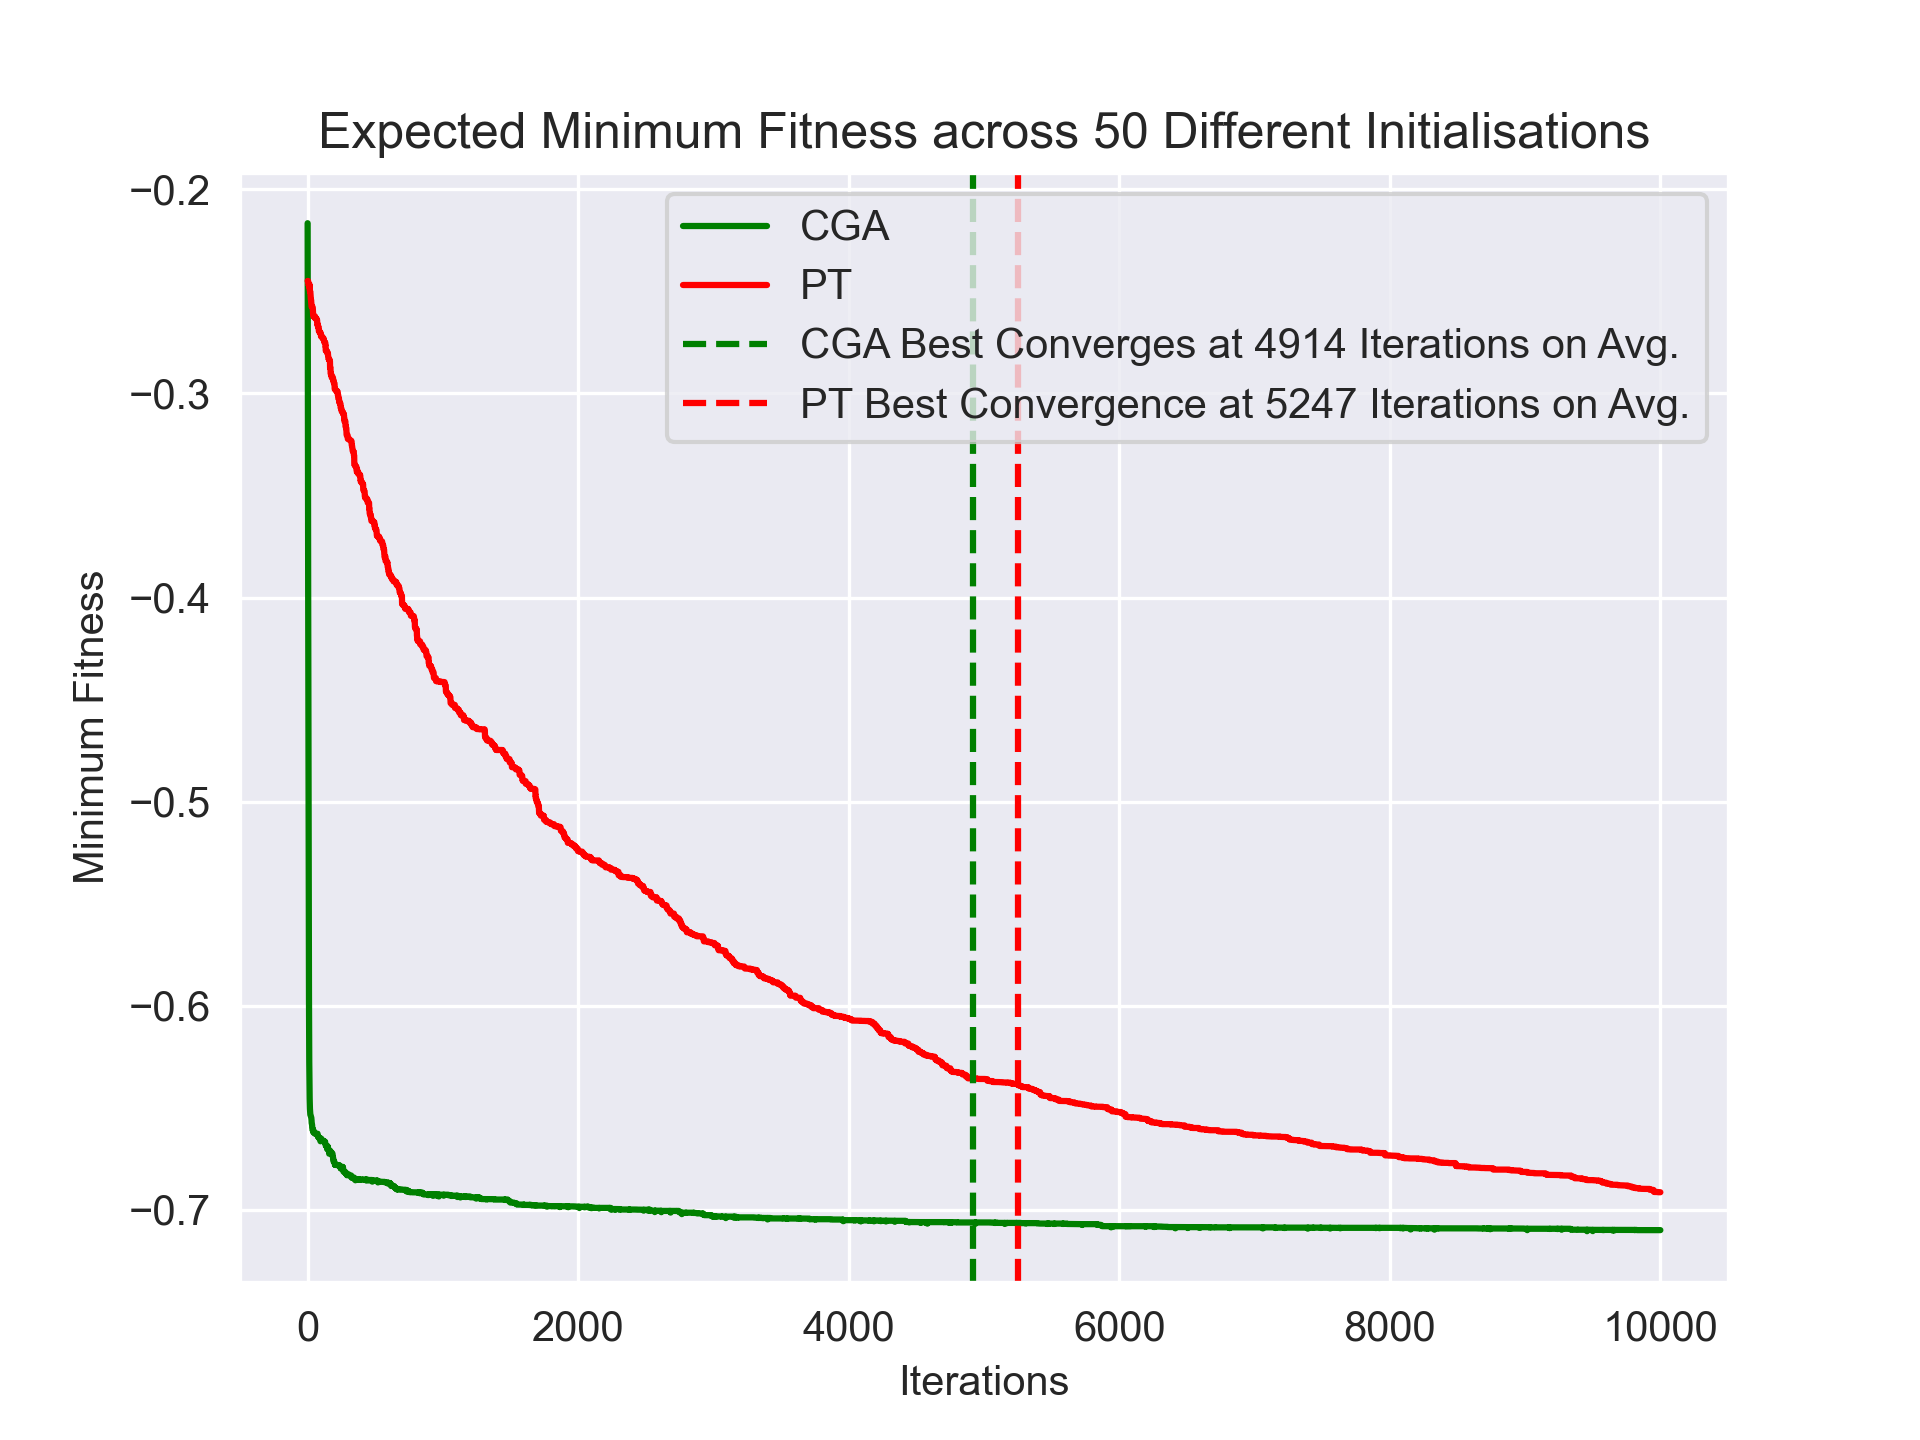
\includegraphics[width=\textwidth]{../figures/Final Comparison/CGA vs PT Minimum Fitness.png}
        \caption{Minimum fitnesses.}
        \label{fig:MIN_final_fitness}
    \end{subfigure}
\captionsetup{justification=centering}
\caption{Evolution of fitness values over 10,000 iterations for the CGA and PT algorithms, using 50 shared initialisations.}
\label{fig:final_fitness}
\end{figure}

The contrast in the mean final fitness values of the optimal solutions amounted to a mere 0.0186, corresponding to a marginal 2.65\% disparity. This slight difference implies that the CGA demonstrated only a modest advantage over the PT algorithm in terms of solution quality after 10,000 iterations. This outcome suggests that the 10,000 iterations was not sufficient for the PT algorithm to thoroughly explore the search space and converge to the global maxima. Although it is challenging to definitively assert that more iterations would have led to global convergence, the observed trend in Fig. \ref{fig:final_fitness} strongly suggests that such convergence was likely, and that the PT algorihtm would have eventually overtaken the CGA.

However, the contrast in the standard deviations of their final minimum fitness values paints a different picture, showcasing a discrepancy of 0.00961, equivalent to 37.5\%. The PT algorithm demonstrated considerably greater stability in reaching its final optimal solution. Although its average fitness across the entire set of solutions displayed more variability than the CGA, this characteristic regarding its optimal solution could confer an advantage to the PT algorithm in specific applications where a slightly inferior optimal objective function evaluation is acceptable in exchange for consistently reliable performance.

Furthermore, an additional noteworthy observation is that the PT algorithm demanded an additional 79.72 seconds to execute the entire 10,000 iterations, representing a substantial 61.2\% increase above the CGA. On average, it also necessitated 332 more iterations for convergence, translating to roughly 44.83 seconds more than the CGA, marking a noteworthy 67.0\% difference. This notable disparity can be ascribed to the inherently more parallel and exploratory approach of the PT algorithm, underscoring that the CGA is better suited for applications prioritising computational efficiency.

Another salient aspect to consider is that the CGA was comparatively simpler to implement than the PT algorithm. However, it is important to acknowledge the potential influence of personal bias, as Genetic Algorithms were covered in the lecture materials, while the PT algorithm was not. Simlarly, accessing literature for inspiration and guidance was markedly easier for the CGA implementation and its adaptions than it was for the PT algorithm. This discrepancy in accessibility presents an additional practical advantage in favor of the CGA.

Overall, the PT algorithm holds promise in consistently attaining the global optimum with extended CPU time. Conversely, the CGA boasts efficiency, quicker convergence, and a simpler implementation process. The selection between these two algorithms hinges on the specific application and the relative significance assigned to these factors.

\subsection{Limitations of this Study}

While the preceding study was purposefully comprehensive and rigorous, there exist significant opportunities for enhancing the reliability and granularity of the results. The following points outline some notable limitations:

\begin{itemize}
    \item \textbf{Limited Exploration of Hyperparameter Space:} The hyperparameter space was explored to a limited extent. The selection of specific parameters for fine-tuning was partly driven by educational objectives and the desire to solidify understanding of the algorithms. The approach, while educational, was not exhaustive, leaving room for further refinement of key parameters like population size, number of parents, tournament size, replica count, and chain count. There is potential to achieve improved and expedited results through more comprehensive hyperparameter tuning.
    \item \textbf{Dimensional Discrepancy:} Hyperparameter tuning was specifically carried out for the two-dimensional KBF. It is crucial to note that the optimal hyperparameters identified for the 2-dimensional KBF may not necessarily be optimal for its 8-dimensional counterpart. This discrepancy represents a limitation in the study, and there is a possibility that results could differ if hyperparameter tuning were conducted for the 8-dimensional KBF. However, the choice to focus on the 2-dimensional KBF for hyperparameter tuning was driven by considerations of computational efficiency and the facilitation of visualisation.
    \item \textbf{Parallelisation:} Despite temptation, parallelisation of the algorithms was deliberately avoided to maintain the reproducibility and comparability of the results. While parallelising the algorithms could have enhanced efficiency, particularly for the PT algorithm, known for its suitability for straightforward parallelisation, its implementation might introduce an unfair advantage and complicate the overall comparison.
    \item \textbf{Algorithmic Choices:} It is worth noting that additional efforts could be directed towards achieving diverse objectives through fine-tuning, beyond merely targeting lower minimum fitness values. Objectives such as faster convergence or reduced standard deviations could be explored. Moreover, there is room for further adaptation of the algorithms to enhance their performance. For instance, the CGA could be modified to include elitism, while the PT algorithm might benefit from modifications involving a more sophisticated temperature schedule.
    \item \textbf{Initialisation:} Considerable literature is available on more sophisticated methods for initialising solutions. The approach employed in this study was relatively simplistic, leaving room for potential enhancements in the quality of initial solutions, with the prospect of subsequently improving the overall performance of the algorithms.
    \item \textbf{Convergence Criterion:} The convergence criterion was determined after a trial run, and it is conceivable that adopting a different criterion might have resulted in varied outcomes. Nonetheless, the chosen criterion aimed to strike a balance, being stringent enough to ensure that the algorithms had converged to an optimum while maintaining leniency to facilitate a fair and meaningful comparison between the two algorithms.
    \item \textbf{Constraints Handling:} The treatment of constraints in both algorithms was notably simplistic, relying on a straightforward rejection method. Considering the intricacy of the constraint boundaries, it might have been beneficial to explore a more sophisticated approach to enhance the overall performance of the algorithms.
    \item \textbf{Reproducibility:} The algorithms were implemented by an individual student and executed on a single machine. Despite efforts to design the code for reproducibility, there is a potential for variation in results if the algorithms were implemented by a different individual or executed on a different machine. To mitigate this limitation, future studies could involve running different algorithms on multiple machines and conducting a comparative analysis of the results.
\end{itemize}
\end{multicols}

\newpage

\section{Conclusions}
\begin{itemize}
    \item Two algorithms, namely the Continuous Genetic Algorithm (CGA) and Parallel Tempering (PT), were introduced and fine-tuned using the 2-dimensional Keane's Bump Function. Subsequently, their performances were comparatively assessed in optimising the 8-dimensional Keane's Bump Function.
    \item The optimal configuration for the CGA comprised a population size of 250, 62 parents at each mating step, tournament selection with a size of 62, a crossover probability of 0.65, and a mutation rate of 0.1. On the other hand, the optimal configuration for PT included 10 replicas exchanging solutions at each iteration, 25 chains, and a uniform temperature schedule.
    \item The CGA greater computational efficiency, completing 10,000 iterations 79.72 seconds faster than the PT algorithm. Additionally, it required 332 fewer iterations to converge, equivalent to approximately 44.83 seconds less than the PT algorithm. However, the PT algorithm demonstrated enhanced stability in reaching its final optimal solution, boasting a standard deviation of 0.03044 compared to the CGA's 0.02083. Notably, the PT algorithm showcased a stronger inclination towards exploration, while the CGA displayed a more exploitative nature. Given more iterations, the PT algorithm was likely to surpass the CGA in discovering the global optima.
    \item The selection between the two algorithms depends on the particular application and the relative importance assigned to factors such as computational efficiency, stability, and solution quality.
    \item Limitations pertaining to the study's scope and implementation were recognised, and potential directions for future work were suggested.
\end{itemize}
\bibliographystyle{plain}
\bibliography{refs} % Entries are in the refs.bib file
\newpage
\section{Appendix}
\subsection{Supplementary Results regarding CGA Tuning}
\label{sec:CGA_tuning_results}
\begin{table}[H]
    \centering
    \begin{tabular}{|*{5}{c|}}
        \hline
        \renewcommand{\arraystretch}{1.5}
        \multirow{2}{*}{\textbf{Selection Method}} & \multirow{2}{*}{\textbf{Mating Procedure}} & \multirow{2}{*}{\textbf{Iterations}} & \multirow{2}{*}{\textbf{Final Avg. Fitness}} & \multirow{2}{*}{\textbf{Final Min. Fitness}} \\
        & & & & \\
        \hline
        \multirow{4}{*}{Proportional} & \multirow{2}{*}{Crossover} & 10 & -0.19890798 & -0.247328018 \\
        & &\cellcolor{lightgray} 100 &\cellcolor{lightgray} -0.212384457 &\cellcolor{lightgray} -0.24867806 \\
        \cline{2-5}
        & \multirow{2}{*}{Heuristic Crossover} & 10 & -0.199296791 & -0.258198948 \\
        & &\cellcolor{lightgray} 100 &\cellcolor{lightgray} -0.22656183 & \cellcolor{lightgray} -0.250977443 \\
        \hline
        \multirow{4}{*}{Tournament} & \multirow{2}{*}{Crossover} & 10 & -0.309572335 & -0.331996331 \\
        & &\cellcolor{lightgray} 100 &\cellcolor{lightgray} -0.309235401 &\cellcolor{lightgray} -0.342745604 \\
        \cline{2-5}
        & \multirow{2}{*}{Heuristic Crossover} & 10 & -0.241261775 & -0.262876797 \\
        & &\cellcolor{lightgray} 100 &\cellcolor{lightgray} -0.247574635 &\cellcolor{lightgray} -0.262876811 \\
        \hline
        \multirow{4}{*}{SRS} & \multirow{2}{*}{Crossover} & 10 & -0.189986008 & -0.208434151 \\
        & &\cellcolor{lightgray} 100 &\cellcolor{lightgray} -0.288766718 &\cellcolor{lightgray} -0.319667279 \\
        \cline{2-5}
        & \multirow{2}{*}{Heuristic Crossover} & 10 & -0.177779432 & -0.207148488 \\
        & &\cellcolor{lightgray} 100 &\cellcolor{lightgray} -0.182101833 &\cellcolor{lightgray} -0.338823558 \\
        \hline
    \end{tabular}
    \captionsetup{justification=centering}
    \caption{Raw results from an initial exploration of the selection method and mutation procedure hyperparameters within the CGA. Presented as the final fitness values of the CGA population after 10 and 100 iterations. Here, minimum fitness refers to the fitness of the best (feasible) individual within the population. Additionally, the mutation rate was set to 0.05, and the crossover probability was set to 0.7.}
    \label{tab:CGAexploration}
\end{table}

\begin{figure}[H]
    \centering
    \begin{subfigure}{0.85\textwidth}
        \centering
        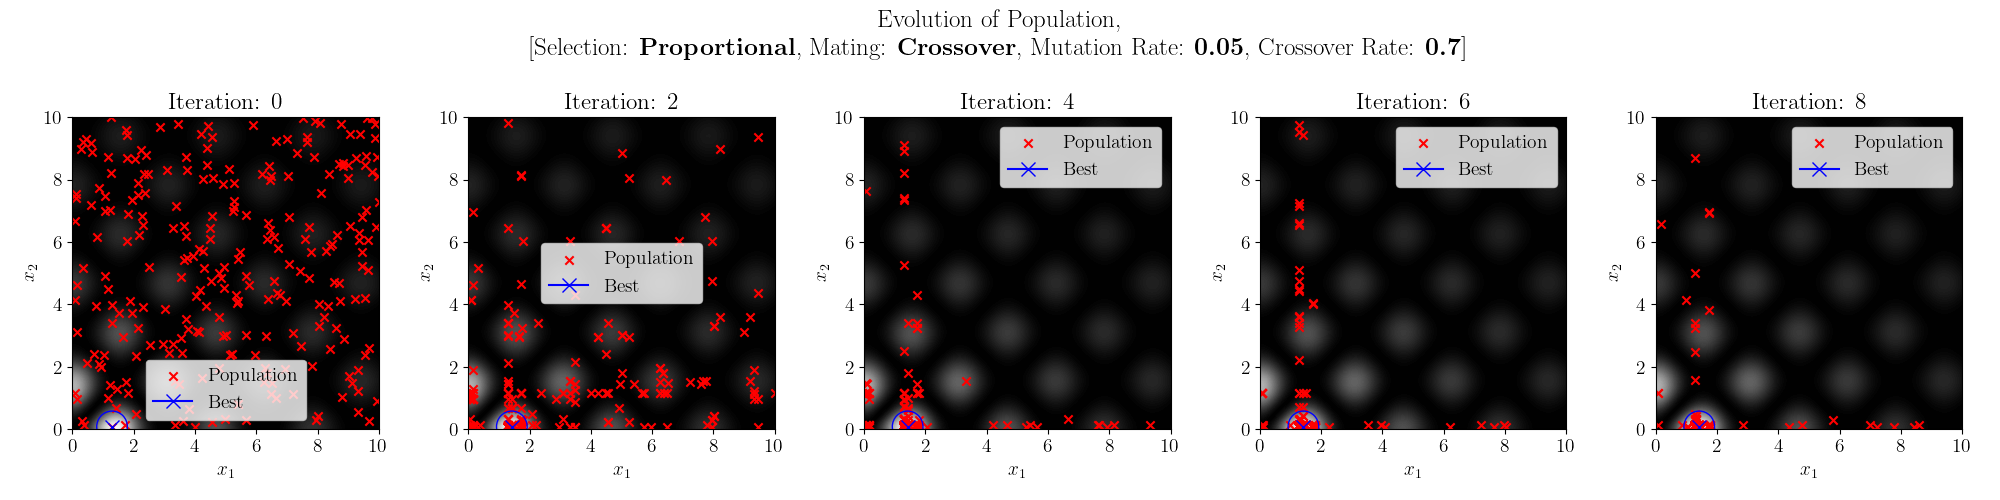
\includegraphics[width=\textwidth]{../figures/KBF/10_iters/Proportional/Crossover/0.05_0.7_Population.png}
        \caption{Mutation Procedure: Crossover}
        \label{fig:CGA_flowchart_proportional_crossover}
    \end{subfigure}
    \begin{subfigure}{0.85\textwidth}
        \centering
        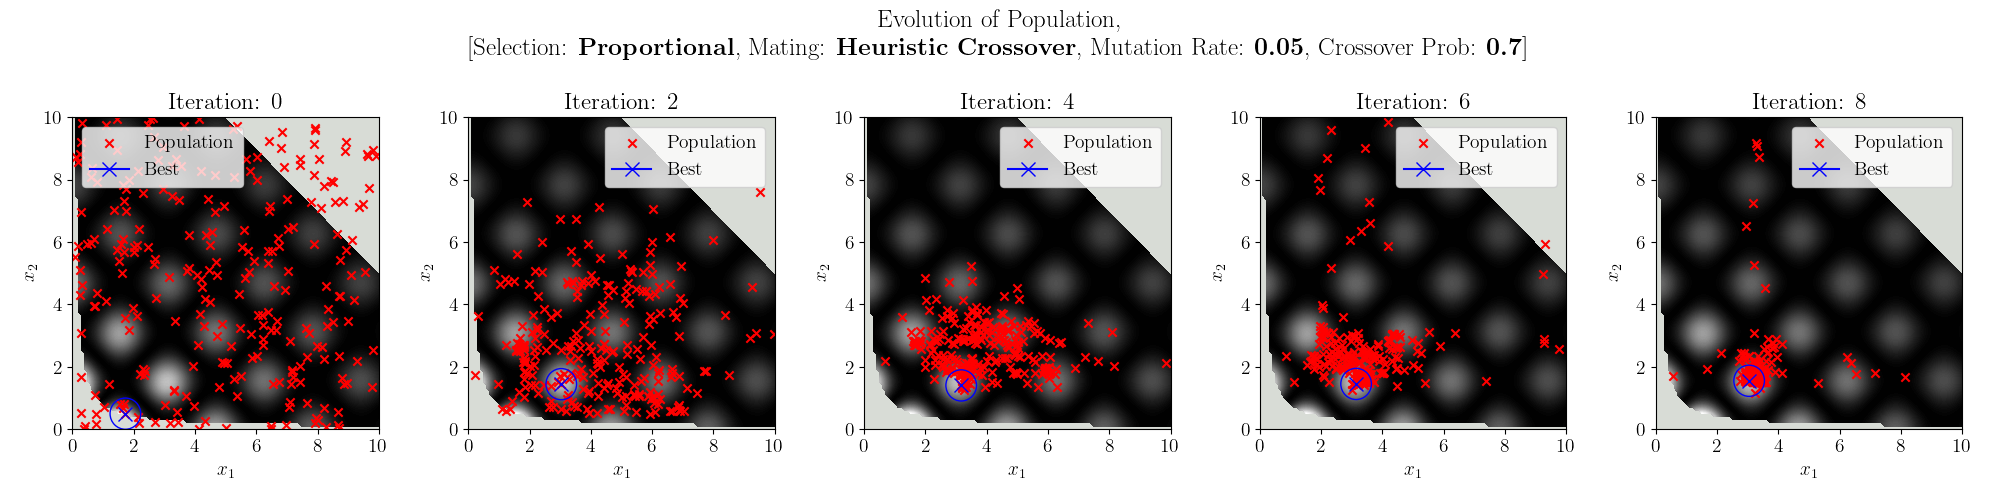
\includegraphics[width=\textwidth]{../figures/KBF/10_iters/Proportional/Heuristic Crossover/0.05_0.7_Population.png}
        \caption{Mutation Procedure: Heuristic Crossover}
        \label{fig:CGA_flowchart_proportional_Heuristic Crossover}
    \end{subfigure}
    \captionsetup{justification=centering}
    \caption{Evolution of the CGA population over 8 iterations using proportional selection. Proportional selection proved to be a somewhat effective selection method. However, it was not chosen over tournament selection as the primary selection method for the reasons outlined in Section \ref{sec:CGA_selection_mutation}.}
    \label{fig:CGA_flowchart_proportional}
\end{figure}

% \begin{figure}[H]
%     \centering
%     \begin{subfigure}{0.85\textwidth}
%         \centering
%         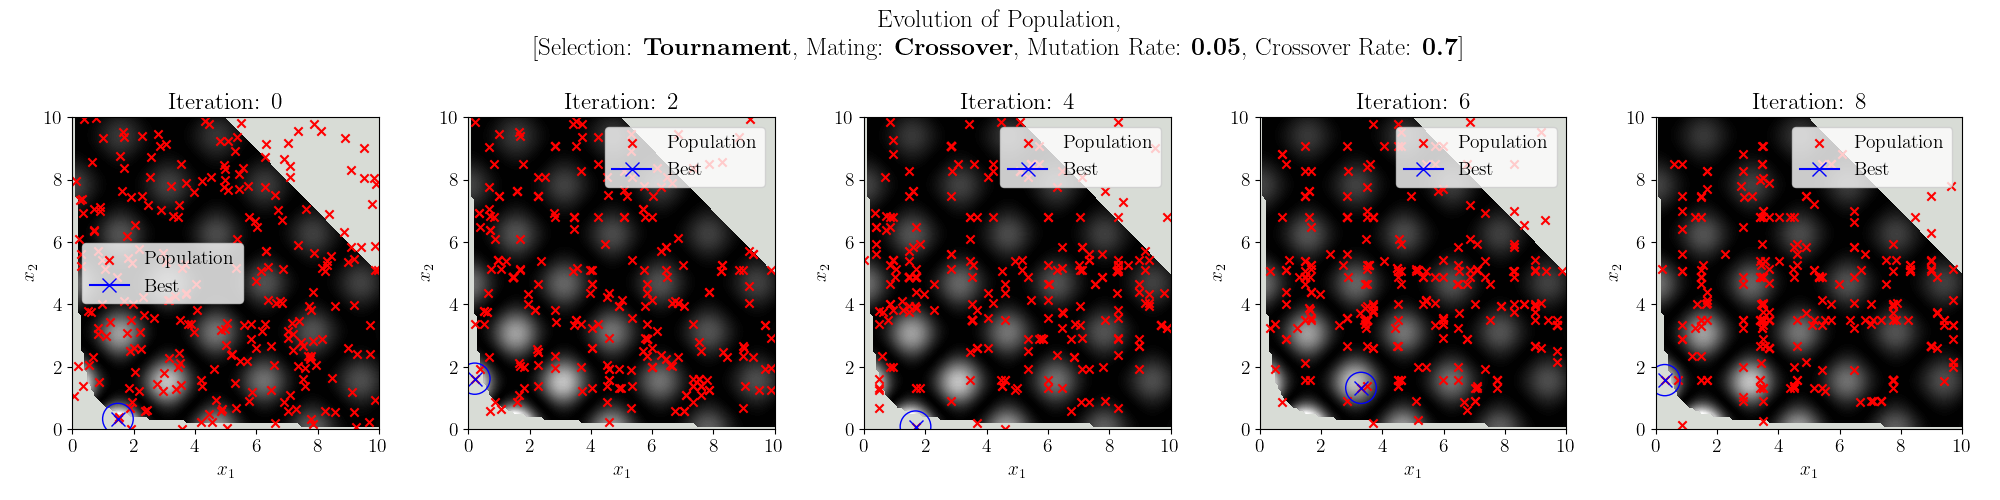
\includegraphics[width=\textwidth]{../figures/KBF/10_iters/Tournament/Crossover/0.05_0.7_Population.png}
%         \caption{Mutation Procedure: Crossover}
%         \label{fig:CGA_flowchart_tournament_crossover}
%     \end{subfigure}
%     \begin{subfigure}{0.85\textwidth}
%         \centering
%         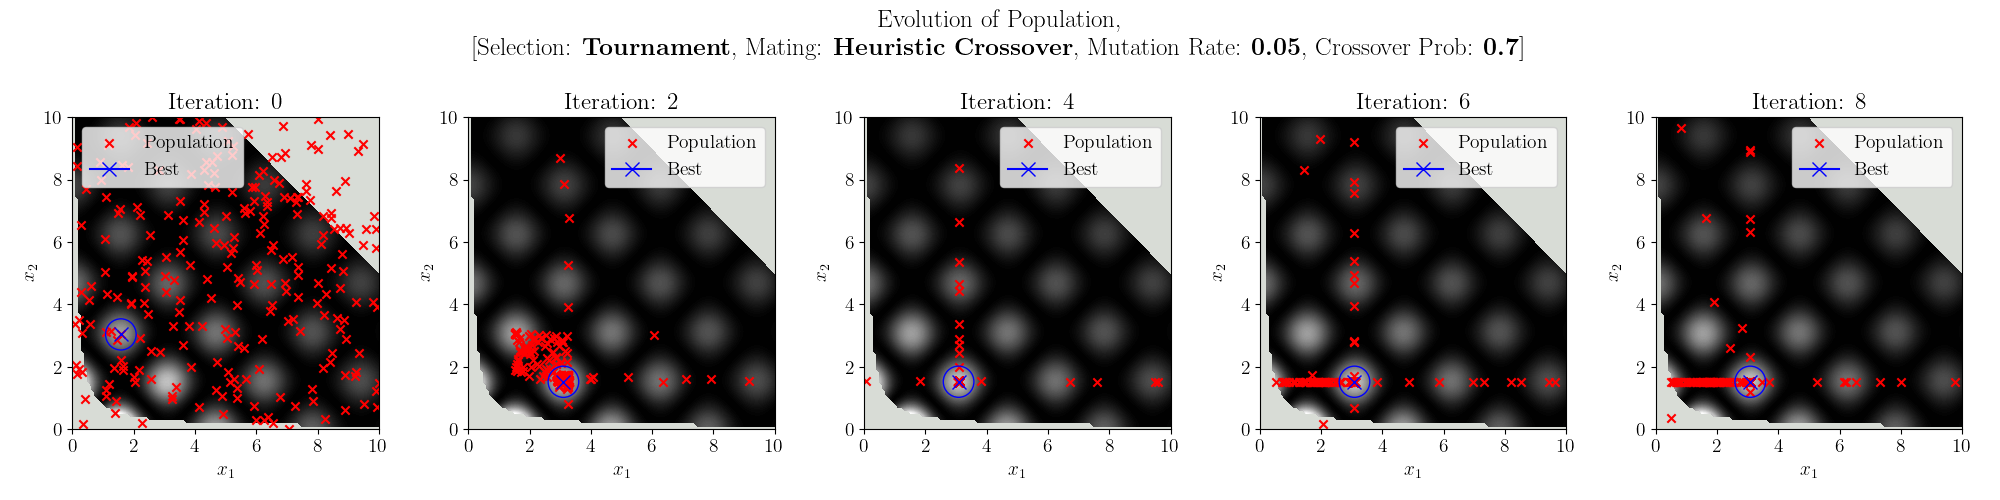
\includegraphics[width=\textwidth]{../figures/KBF/10_iters/Tournament/Heuristic Crossover/0.05_0.7_Population.png}
%         \caption{Mutation Procedure: Heuristic Crossover}
%         \label{fig:CGA_flowchart_tournament_Heuristic Crossover}
%     \end{subfigure}
%     \captionsetup{justification=centering}
%     \caption{Evolution of the CGA population over 8 iterations using tournament selection. Tournament selection proved to be the most effective selection method, when compared to Proportional Selection and Stochastic Remainder Selection without Replacement (SRS), as discussed in \ref{sec:CGA_selection_mutation}.}
%     \label{fig:CGA_flowchart_tournament}
% \end{figure}

\begin{figure}[H]
    \centering
    \begin{subfigure}{0.85\textwidth}
        \centering
        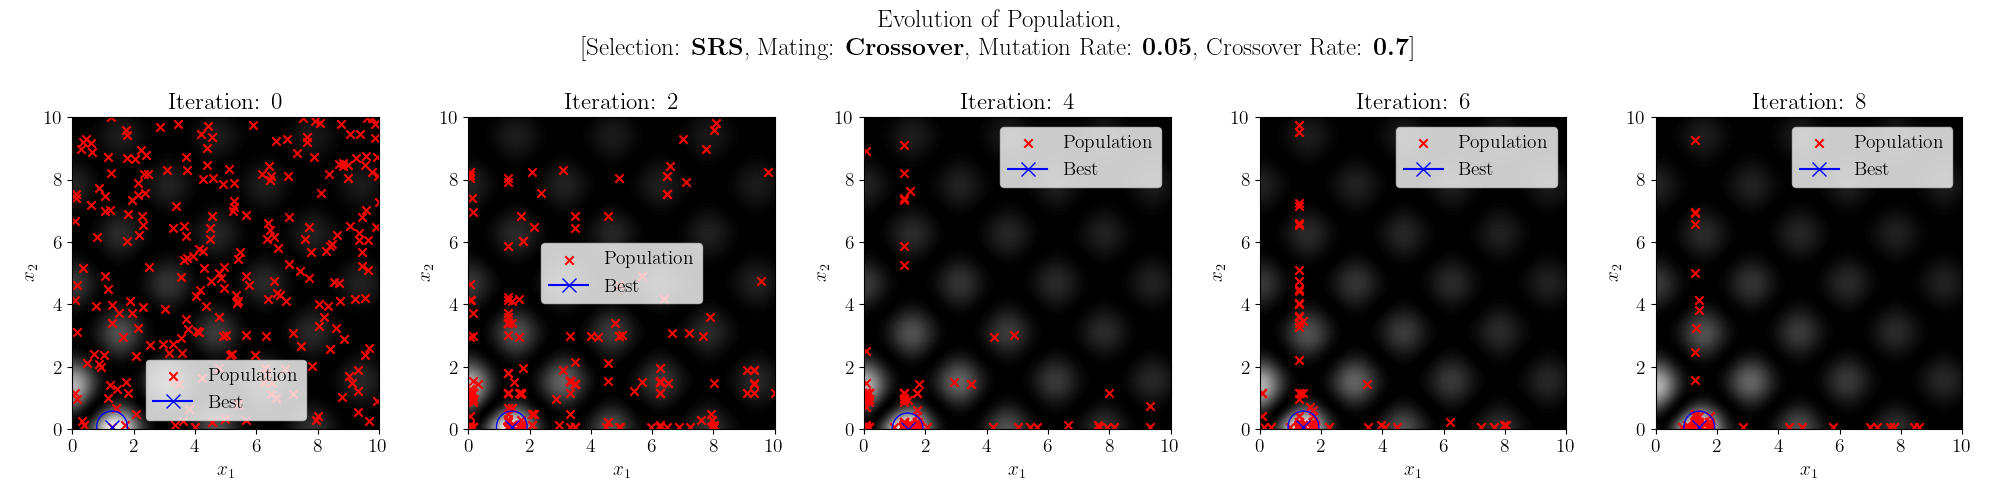
\includegraphics[width=\textwidth]{../figures/KBF/10_iters/SRS/Crossover/0.05_0.7_Population.png}
        \caption{Mutation Procedure: Crossover}
        \label{fig:CGA_flowchart_SRS_crossover}
    \end{subfigure}
    \begin{subfigure}{\textwidth}
        \centering
        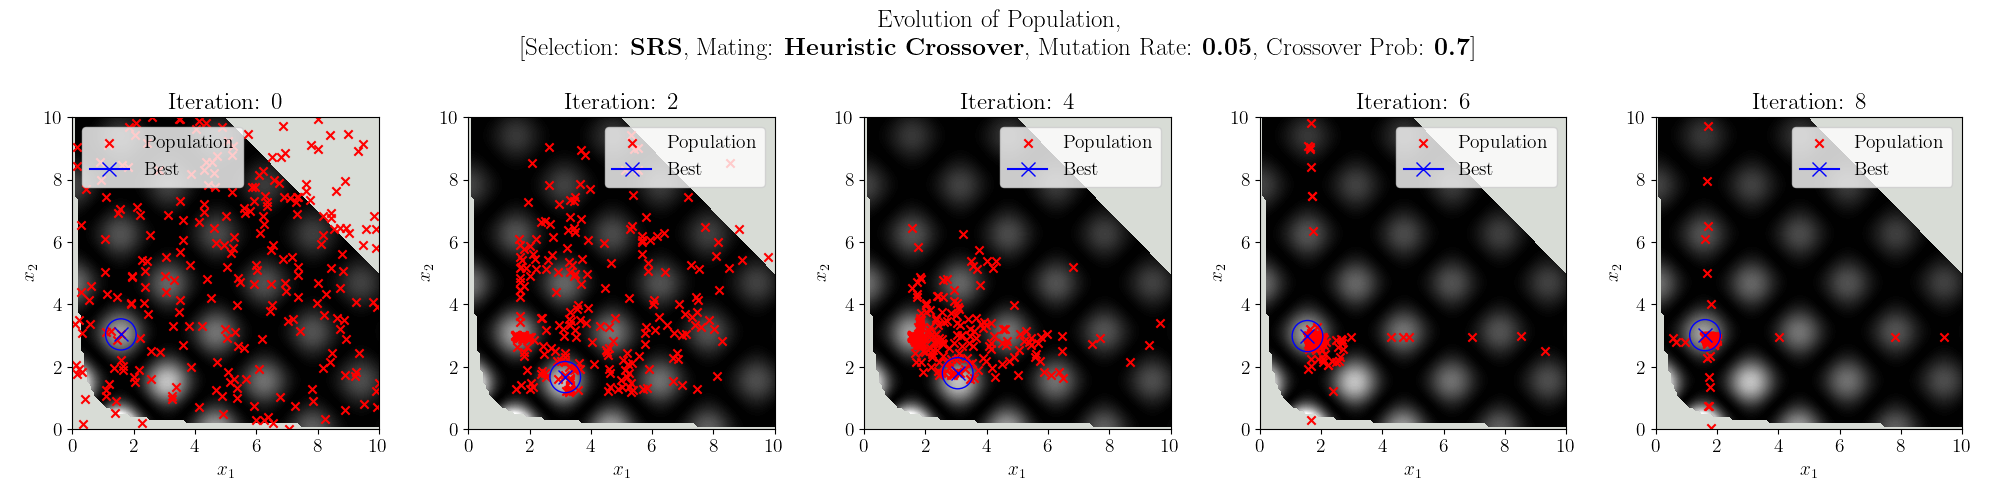
\includegraphics[width=0.85\textwidth]{../figures/KBF/10_iters/SRS/Heuristic Crossover/0.05_0.7_Population.png}
        \caption{Mutation Procedure: Heuristic Crossover}
        \label{fig:CGA_flowchart_SRS_Heuristic Crossover}
    \end{subfigure}
    \captionsetup{justification=centering}
    \caption{Evolution of the CGA population over 8 iterations using stochastic remainder selection without replacement (SRS). SRS proved to be the second most effective selection method, when compared to Proportional Selection and Tournament Selection, as discussed in \ref{sec:CGA_selection_mutation}.}
    \label{fig:CGA_flowchart_SRS}
\end{figure}

\subsection{Supplementary Results regarding PT Tuning}
\label{sec:PT_tuning_results}

\begin{table}[H]
    \centering
    \begin{tabular}{|*{5}{c|}}
        \hline
        \multirow{3}{*}{Exchange Procedure} & \multirow{3}{*}{\shortstack{Exchange\\Parameter}} & \multirow{3}{*}{Power Term} & \multirow{3}{*}{Final Avg. Fitness} & \multirow{3}{*}{Final Min. Fitness} \\
        & & & & \\
        & & & & \\
        \hline
        \multirow{9}{*}{Periodic} & \multirow{3}{*}{0.1} & 1 & -0.186415811 & -0.34081297 \\
        & & 3\cellcolor{lightgray} & -0.186415811\cellcolor{lightgray} & -0.34081297\cellcolor{lightgray} \\
        & & 5\cellcolor{gray} & -0.192142049\cellcolor{gray} & -0.34081297\cellcolor{gray} \\
        \cline{2-5}
        & \multirow{3}{*}{0.3} & 1 & -0.183591253 & -0.335207939 \\
        & & 3\cellcolor{lightgray} & -0.183591253\cellcolor{lightgray} & -0.335207939\cellcolor{lightgray} \\
        & & 5\cellcolor{gray} & -0.178574074\cellcolor{gray} & -0.310814711\cellcolor{gray} \\
        \cline{2-5}
        & \multirow{3}{*}{0.5} & 1 & -0.166370319 & -0.355617525 \\
        & & 3\cellcolor{lightgray} & -0.166370319\cellcolor{lightgray} & -0.355617525\cellcolor{lightgray} \\
        & & 5\cellcolor{gray} & -0.162769374\cellcolor{gray} & -0.31189813\cellcolor{gray} \\
        \hline
        \multirow{9}{*}{Stochastic} & \multirow{3}{*}{0.1} & 1 & -0.182496471 & -0.327434397 \\
        & & 3\cellcolor{lightgray} & -0.182496471\cellcolor{lightgray} & -0.327434397\cellcolor{lightgray} \\
        & & 5\cellcolor{gray} & -0.197887075\cellcolor{gray} & -0.328011329\cellcolor{gray} \\
        \cline{2-5}
        & \multirow{3}{*}{0.3} & 1 & -0.191162383 & -0.310872726 \\
        & & 3\cellcolor{lightgray} & -0.191162383\cellcolor{lightgray} & -0.310872726\cellcolor{lightgray} \\
        & & 5\cellcolor{gray} & -0.196042151\cellcolor{gray} & -0.314329893\cellcolor{gray} \\
        \cline{2-5}
        & \multirow{3}{*}{0.5} & 1 & -0.206621007 & -0.347483314 \\
        & & 3\cellcolor{lightgray} & -0.206621007\cellcolor{lightgray} & -0.347483314\cellcolor{lightgray} \\
        & & 5\cellcolor{gray} & -0.211224821\cellcolor{gray} & -0.349273739\cellcolor{gray} \\
        \hline
    \end{tabular}\
    \captionsetup{justification=centering}
    \caption{Raw results from an initial exploration of the exchange procedure, exchange parameter, and power term hyperparameters within PT. Presented as the final fitness values of the PT solutions after 100 iterations. Here, minimum fitness refers to the fitness of the best (feasible) solution across all chains.}
    \label{tab:exchange_results}
\end{table}

\begin{figure}[H]
    \centering
    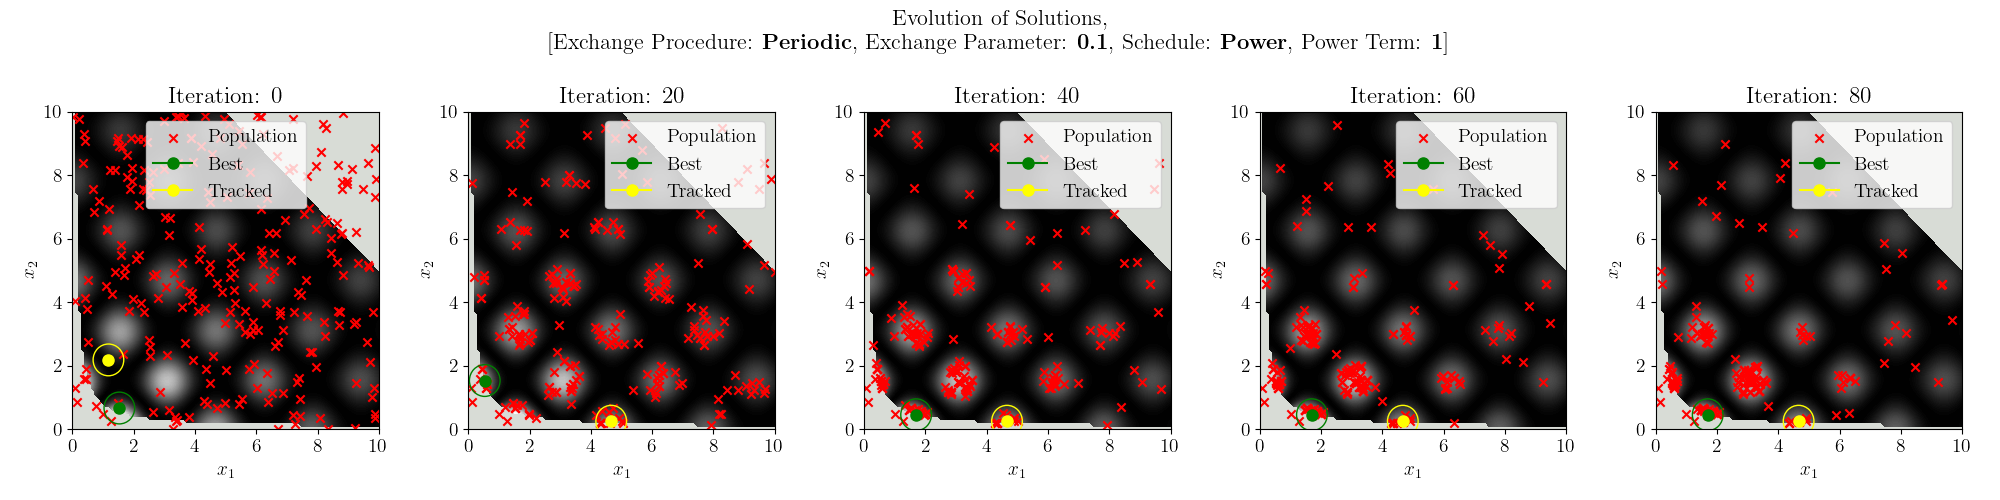
\includegraphics[width=0.85\textwidth]{../figures/KBF/100_iters/Periodic/Power/0.1_1_Solutions.png}
    \captionsetup{justification=centering}
    \caption{Evolution of the chain across all replicas over 100 iterations using periodic replica exchange and a uniform temperature scheduling, (power term of 1). Here, replica exchange occurs every 10\% of the time, (exchange parameter set to 0.1). The 'tracked' solution is distinct from the 'best' solution. It is a random solution within the final replica that is observed to verify the MCMC evolution.}
    \label{fig:PeriodicApp}
\end{figure}

\begin{figure}[H]
    \centering
    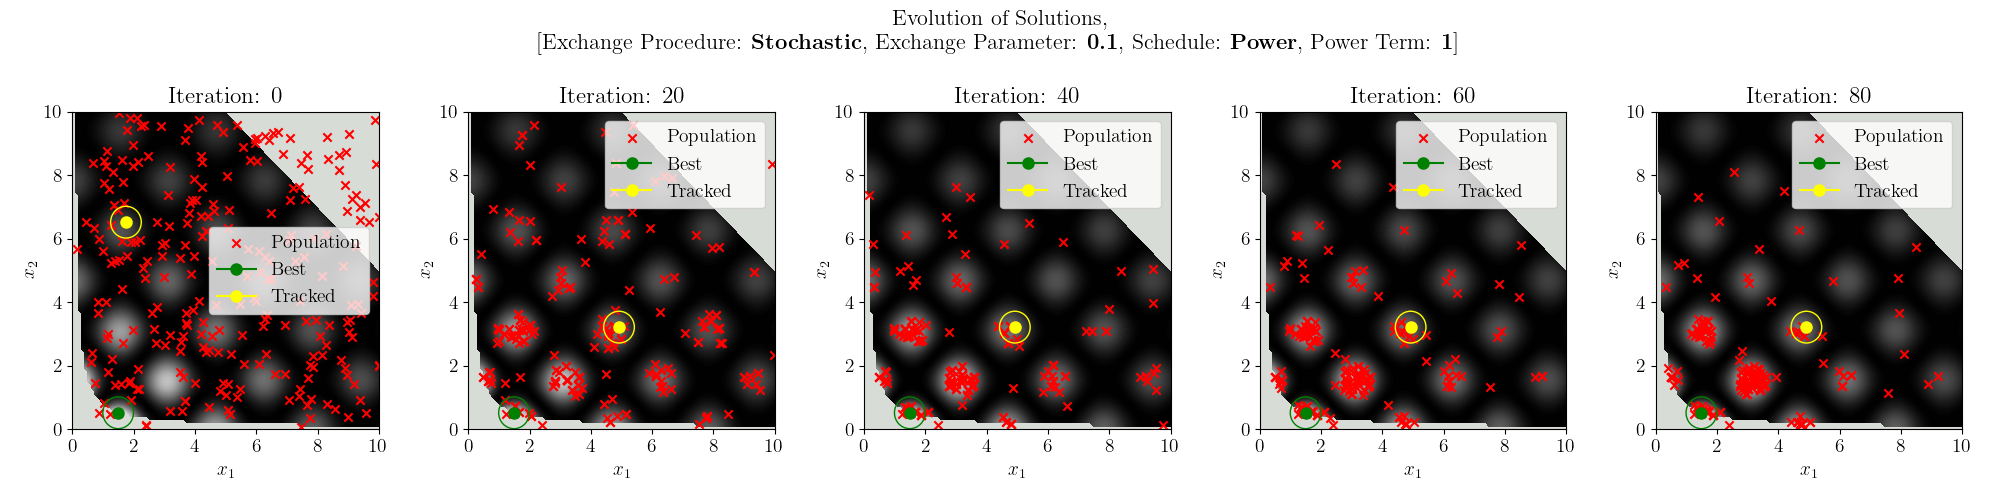
\includegraphics[width=0.85\textwidth]{../figures/KBF/100_iters/Stochastic/Power/0.1_1_Solutions.png}
    \captionsetup{justification=centering}
    \caption{Evolution of the chain across all replicas over 100 iterations using stochastic replica exchange and a uniform temperature scheduling, (power term of 1). Here, replica exchange occurs with a probability of 10\%.  The 'tracked' solution is distinct from the 'best' solution. It is a random solution within the final replica that is observed to verify the MCMC evolution.}
    \label{fig:StochasticApp}
\end{figure}
\vspace{-3.5mm}
\section{Code}
\label{sec:code}

To ease development, the codebase has been modularised in the manner presented below:

\begin{itemize}
    \footnotesize
    \item[] \href{#sec:algorithms}{\textit{src/}}
    \begin{itemize}
        \item[] \href{#sec:CGA}{\textit{algorithms/}}
        \begin{itemize}
            \item[] \href{#sec:CGA}{\textit{CGA/}}
            \begin{itemize}
                \item[] \href{#CGApy}{\textit{CGA.py}}
                \item[] \href{#mating_functionspy}{\textit{mating\_functions.py}}
                \item[] \href{#selection_functionspy}{\textit{selection\_functions.py}}
            \end{itemize}
            \item[] \href{#sec:PT}{\textit{PT/}}
            \begin{itemize}
                \item[] \href{#PTpy}{\textit{PT.py}}
                \item[] \href{#replica_exchange_functionspy}{\textit{replica\_exchange\_functions.py}}
                \item[] \href{#temp_prog_functionspy}{\textit{temp\_prog\_functions.py}}
            \end{itemize}
        \end{itemize}
        \item[] \href{#sec:utils}{\textit{utils/}}
        \begin{itemize}
            \item[] \href{#helper_functionspy}{\textit{helper\_functions.py}}
            \item[] \href{#plotting_functionspy}{\textit{plotting\_functions.py}}
        \end{itemize}
        \item[] \href{#functions.py}{\textit{functions.py}}
    \end{itemize}
    \item[] \href{#FinalComparison.py}{\textit{FinalComparison.py}}
    \item[] \href{#CGA_TuningExperiments.py}{\textit{CGA\_TuningExperiments.py}}
    \item[] \href{#PT_TuningExperiments.py}{\textit{PT\_TuningExperiments.py}}
\end{itemize}

\subsection{algorithms}
\label{sec:algorithms}
\subsubsection{CGA}
\label{sec:CGA}
\begin{lstlisting}[language=Python, caption=CGA.py, label=CGApy]
"""
Candidate No : 5730E, Module: 4M17 

Description :
    This file contains the class for the continous genetic algorithm.
"""

import numpy as np
import sys; sys.path.append('..')

from src.algorithms.CGA.selection_functions import proportional_selection, tournament_selection, SRS_selection
from src.algorithms.CGA.mating_functions import crossover, heuristic_crossover
from src.utils.helper_functions import satisfy_constraints

class ContinousGeneticAlgorithm():
    """
    Class for continous genetic algorithm.  
    """
    def __init__(self, population_size, chromosome_length, num_parents, objective_function, tournament_size, range=(0,10), mutation_rate=0.1, crossover_prob=0.8, selection_method='Tournament', mating_procedure='Heuristic Crossover', constraints=True):
        """
        Constructor for continous genetic algorithm.

        Parameters:
        - population_size (int): Number of individuals in population    
        - chromosome_length (int): Size of vector individual, (number of genes), i.e. dimension of solution space
        - num_parents (int): Number of parents to select for mating
        - objective_function (function): Objective function to optimise
        - tournament_size (int): Size of subset of population for tournament selection
        - range (tuple): Range of values for genes, determined by constraints of problem
        - mutation_rate (float): Mutation rate
        - crossover_prob (float): Crossover rate
        - selection_method (str): Selection method used for parent selection
        - mating_procedure (str): Mating procedure used for reproduction
        - constraints (bool): Whether to satisfy constraints with parent selection or not
        """
        self.population_size = population_size 
        self.chromosome_length = chromosome_length # n in R^n, dimension of the search space
        self.num_parents = num_parents
        self.func = objective_function
        self.tournament_size = tournament_size
        self.lb = range[0] 
        self.ub = range[1] 
        self.mutation_rate = mutation_rate  
        self.crossover_prob = crossover_prob
        self.constraints = constraints
        
        # Dictionaries to map string to function call. Function imported from directory files
        selection_mapping = {'Proportional': proportional_selection, 
                            'Tournament': tournament_selection, 
                            'SRS': SRS_selection # SRS = Stochastic Remainder Selection without Replacement
                            } 
        
        mating_mapping = {'Crossover': crossover,
                          'Heuristic Crossover': heuristic_crossover 
                          }

        # Check if selection method and mating procedure are valid
        if selection_method not in ['Proportional', 'Tournament', 'SRS']:
            raise ValueError(f"Invalid selection method: {selection_method}")
        else:
            self.selection_process = selection_mapping[selection_method]

        if mating_procedure not in ['Crossover', 'Heuristic Crossover']:
            raise ValueError(f"Invalid mating procedure: {mating_procedure}")
        else:
            self.mating_process = mating_mapping[mating_procedure]

        # Initialise population
        self.initialise_population() 
        
    def initialise_population(self):
        """
        Initialise population with random values between lb and ub.
        """
        self.population = np.random.uniform(low=self.lb, 
                                            high=self.ub, 
                                            size=(self.population_size, self.chromosome_length)
                                            )
        
        self.fitness = np.zeros(self.population_size) # Initialise fitness of population
        self.evaluate_fitness() # Update fitness of population with starting individual

    def evaluate_fitness(self):
        """
        Evaluate fitness of population.

        Parameters:
        - fitness_function (function): Fitness function to evaluate fitness of population
        """
        for i in range(self.population_size):
            self.fitness[i] = - self.func(self.population[i])

        # Evaluate rankings of individuals in population by fitness
        self.parent_rankings = np.argsort(self.fitness) # Indices of individuals in order of fitness

        # Update best individual and best fitness
        self.best_individual = self.population[self.parent_rankings[0]]
        self.min_fitness = self.fitness[self.parent_rankings[0]]

        # Best individual must satisfy constraints, if not, find next best individual that does
        i = 1
        while not satisfy_constraints(self.best_individual):
            self.best_individual = self.population[self.parent_rankings[i]]
            self.min_fitness = self.fitness[self.parent_rankings[i]]
            i += 1
            
    def select_parents(self):
        """
        Select parents for mating.

        Returns:
        - parents (np.array): Indices of parents selected for mating
        """
        return self.selection_process(self)

    def mate(self):
        """
        Mate parents to produce offspring.

        Returns:
        - offspring (np.array): Offspring of parents
        """
        return self.mating_process(self)

    def mutate(self):
        """
        Mutate offspring. Every gene has a mutation rate chance of being mutated.
        """
        for i in range(self.population_size):
            for j in range(self.chromosome_length):
                if np.random.rand() < self.mutation_rate:
                    self.population[i][j] = np.random.uniform(low=self.lb, high=self.ub)

    def evolve(self):
        """
        Evolve population for one generation.
        """
        offspring = self.mate()
        self.population = offspring
        self.mutate()
        self.evaluate_fitness() 
\end{lstlisting}
\begin{lstlisting}[language=Python, caption=mating\_functions.py, label=mating_functionspy]
    """
    Candidate No : 5730E, Module: 4M17 
    
    This file contains the mating functions for the CGA algorithm.
    """
    
    import numpy as np
    
    def crossover(CGA):
        """
        Crossover mating procedure. 
        """
        # Select parents
        selected_parents = CGA.select_parents()
    
        # Reshape them into a set of potential parent pairs
        parent_pairs = np.array(selected_parents).reshape(-1, 2)
    
        # Initialise new offspring to replace population
        offspring = np.zeros((CGA.population_size, CGA.chromosome_length))
    
        # Iterate through population
        for i in range(CGA.population_size):
    
            # Assign random pair of parents from parent_pairs
            parent1, parent2 = parent_pairs[np.random.randint(len(parent_pairs))]
    
            # Assign random crossover point
            p = np.random.randint(1, CGA.chromosome_length)
    
            # Swap genes from parents to create offspring
            if np.random.rand() < CGA.crossover_prob:
                offspring[i][:p] = CGA.population[parent1][:p]
                offspring[i][p:] = CGA.population[parent2][p:]
            else:
                offspring[i][:p] = CGA.population[parent2][:p]
                offspring[i][p:] = CGA.population[parent1][p:]
    
        return offspring
    
    def heuristic_crossover(CGA):
        """
        Heuristic crossover mating procedure. Inspired by the relevant section in https://doi.org/10.1002/0471671746.ch3
        """
    
        # Select parents
        selected_parents = CGA.select_parents()
    
        # Reschape them into a set of potential parent pairs
        parent_pairs = np.array(selected_parents).reshape(-1, 2)
    
        # Initialise new offspring to replace population
        offspring = np.zeros((CGA.population_size, CGA.chromosome_length))
    
        # Iterate through population
        for i in range(CGA.population_size):
    
            # Assign random pair of parents from parent_pairs
            parent1, parent2 = parent_pairs[np.random.randint(len(parent_pairs))]
            
            # Iterate through all the genes of an individual/chromosome
            for j in range(CGA.chromosome_length):
                
                # Heuristic crossover with probability, CGA.crossover_prob
                b = np.random.rand() # b is a random number between 0 and 1
    
                if np.random.rand() < CGA.crossover_prob:
                    # p_new = b * (p1 - p2) + p2 
                    offspring[i][j] = b * (CGA.population[parent1][j] - CGA.population[parent2][j]) + CGA.population[parent2][j]     
                else:
                    # p_new = b * (p2 - p1) + p1
                    offspring[i][j] = b * (CGA.population[parent2][j] - CGA.population[parent1][j]) + CGA.population[parent1][j]
                    
        return offspring    
\end{lstlisting}
\begin{lstlisting}[language=Python, caption=selection\_functions.py, label=selection_functionspy]
    """
    Candidate No : 5730E, Module: 4M17 
    
    This file contains the selection functions for the CGA algorithm.
    """
    
    import numpy as np
    import sys; sys.path.append('..')
    from src.utils.helper_functions import satisfy_constraints
    
    def proportional_selection(GCA):
        """
        Proportional selection of parents. 
    
        Args:
        - GCA (CGA): Continuous Genetic Algorithm object passed into this function using self.select_parents(self)
    
        Returns:
        - selected_individuals (list): List of indices of selected individuals for mating, length = GCA.num_parents
        """
        # Calculate probabilities
        probabilities = GCA.fitness / np.sum(GCA.fitness)
    
        # Select individuals based on probabilities
        selected_individuals = list(np.random.choice(GCA.population_size, size=GCA.num_parents, p=probabilities))
    
        # Retry - reject parents that do not satisfy constraints
        if GCA.constraints == True:
            for i in range(GCA.num_parents):
                while not satisfy_constraints(GCA.population[selected_individuals[i]]):
                    selected_individuals[i] = np.random.choice(GCA.population_size, p=probabilities)
        
        return selected_individuals
    
    def tournament_selection(GCA):
        """
        Tournament selection of parents. 
    
        Args:
        - GCA (CGA): Continuous Genetic Algorithm object passed into this function using self.select_parents(self)
    
        Returns:
        - selected_individuals (list): List of indices of selected individuals for mating, length = GCA.num_parents
        """
    
        # Initialise list of selected individuals
        selected_individuals = []
    
        # Select top two parents for each tournament, so need 'GCA.num_parents // 2' tournaments
        for i in range(GCA.num_parents//2):
    
            # Take subset of population
            subset = np.random.choice(GCA.population_size, size=GCA.tournament_size, replace=False)
    
            # Take top two parents
            parent1 = subset[np.argmin(GCA.fitness[subset])]
            subset = np.delete(subset, np.argmin(GCA.fitness[subset]))
            parent2 = subset[np.argmin(GCA.fitness[subset])]
    
            # Retry, reject parents that do not satisfy constraints
            if GCA.constraints == True:
                while not satisfy_constraints(GCA.population[parent1]):
                    subset = np.delete(subset, np.argmin(GCA.fitness[subset]))
                    parent1 = subset[np.argmin(GCA.fitness[subset])]
                while not satisfy_constraints(GCA.population[parent2]):
                    subset = np.delete(subset, np.argmin(GCA.fitness[subset]))
                    parent2 = subset[np.argmin(GCA.fitness[subset])]
    
            # Add parents to list of selected individuals
            selected_individuals += [parent1, parent2]
    
        return selected_individuals
    
    def SRS_selection(GCA):
        """
        Stochastic Remainder Selection without Replacement (SRS) of parents. 
    
        Args:
        - GCA (CGA): Continuous Genetic Algorithm object passed into this function using self.select_parents(self)
    
        Returns:
        - selected_individuals (list): List of indices of selected individuals for mating, length = GCA.num_parents
        """
    
        # Calculate probabilities
        probabilities = GCA.fitness / np.sum(GCA.fitness)
    
        # Calculate expected number of copies of each individual
        expected_num_copies = probabilities * GCA.num_parents
    
        # Calculate integer number of copies of each individual
        num_copies = np.floor(expected_num_copies) 
    
        # Calculate remainder, which later serves as the probability of further selection
        remainder = expected_num_copies - num_copies
    
        # Initialise list of selected individuals
        selected_individuals = []
    
        # Duplicate individuals "num_copies" times
        for i in range(GCA.population_size):
    
            # Add only feasible individuals
            if satisfy_constraints(GCA.population[i]):
                selected_individuals += [i] * int(num_copies[i]) # Add i to list num_copies[i] times
    
        # Remainer must satisfy sum(remainder) = 1, since it serves as the probabilities for further selection
        remainder = remainder / np.sum(remainder)
    
        # Calculate remaining number of individuals that need to be selected
        remaining_number = GCA.num_parents - len(selected_individuals)
        
        # Cannot be negative
        remaining_number = remaining_number if remaining_number > 0 else 0
    
        # Select individuals using remainder probabilities
        selected_individuals += list(np.random.choice(GCA.population_size, size=remaining_number, p=remainder))
    
        # Reject parents that do not satisfy constraints
        if GCA.constraints == True:
            for i in range(len(selected_individuals)):
                while not satisfy_constraints(GCA.population[selected_individuals[i]]):
                    selected_individuals[i] = np.random.choice(GCA.population_size, p=remainder)
        
        return selected_individuals    
\end{lstlisting}
\subsubsection{PT}
\label{sec:PT}
\begin{lstlisting}[language=Python, caption=PT.py, label=PTpy]
    """
    Candidate No : 5730E, Module: 4M17 
    
    Description :
        This file contains the class for the parallel tempering algorithm.
    """
    import numpy as np
    
    import sys; sys.path.append('..')
    from src.algorithms.PT.temp_prog_functions import power_progression, geometric_progression
    from src.algorithms.PT.replica_exchange_functions import period_exchange, stochastic_exchange, always_exchange
    from src.utils.helper_functions import satisfy_constraints
    
    class ParallelTempering():
        """
        Class for parallel tempering algorithm.  
        """
        def __init__(self, objective_function, x_dim, range=(0,10), alpha=0.1, omega=2.1, num_replicas=10, num_chains=25, exchange_procedure='Periodic', exchange_param=0.2, schedule_type='Power', power_term=1, total_iterations=100, constraints=True):
            """
            Constructor for parallel tempering algorithm.
    
            Parameters:
            - objective_function (function): Objective function to optimise
            - x_dim (int): Dimension of solution space
            - range (tuple): Range of values for x, determined by constraints of problem
            - alpha (float): Dampening constant for max. allowable step size update
            - omega (float): Weighting for max. allowable step size update
            - num_replicas (int): Number of replicas
            - num_chains (int): Number of solutions per replica
            - exchange_procedure (str): Procedure for exchanging solutions between replicas
            - exchange_param (float between 0 and 1): 
                if exchange_procedure = 'Periodic', this is the percentage of iterations after which to exchange solutions
                if exchange_procedure = 'Stochastic', this is the probability of exchanging solutions between replicas during each iteration
            - progression_type (str): Type of progression for temperature scheduling
            - power_term (float > 1): Temperature progression power term, if using power progression. Schedule is (i/N)^power_term
            - total_iterations (int): Total number of iterations the algorithm will run for
            - constraints (bool): Whether to satisfy constraints with Metropolis criterion or not
            """
            self.func = objective_function
            self.x_dim = x_dim
            self.lb = range[0] 
            self.ub = range[1]
            self.alpha = alpha
            self.omega = omega 
            self.num_replicas = num_replicas
            self.num_chains = num_chains
            self.exchange_param = exchange_param
            self.total_iterations = total_iterations
            self.constraints = constraints
    
            # The update step suggested by Parks et al. (1990) requires control variables to be scaled to [0, 1]
            # Therefore, we need to scale up solutions to original range when evaluating the objective function
            self.scale_up = lambda x: x * (self.ub - self.lb) + self.lb
    
            # Energy difference = (f(x_new) - f(x)) / (k * d * T), the term in the exponent of the Metropolis criterion
            k = 1.38064852e-23 # Boltzmann constant
            self.deltaE = lambda x, x_new, d, T: (self.func(self.scale_up(x_new)) - self.func(self.scale_up(x))) / (k * d * T)
            
            # Check if temperature schedule type is valid
            if schedule_type not in ['Geometric', 'Power']:
                raise ValueError("Invalid progression type")
            
            # Dictionaries to map string to function call. Function imported from directory files
            schedule_mapping = {'Geometric': geometric_progression, 
                                   'Power': power_progression
                                   }
            
            # Check if power term is valid, if it's needed
            if schedule_type == 'Power':
                if power_term is None or power_term < 1:
                    raise ValueError(f"Power term not specified correctly: {power_term}. Must be greater than 1.")
    
            # Generate temperature schedule
            self.temperature_schedule = schedule_mapping[schedule_type](num_replicas, power_term)
    
            # Check if exchange procedure is valid
            if exchange_procedure not in ['Periodic', 'Stochastic', 'Always']:
                raise ValueError(f"Invalid exchange procedure: {exchange_procedure}.")
             
            # Check if exchange parameter is valid, should be either a probability or a percentage
            if exchange_param < 0 or exchange_param > 1:
                raise ValueError(f"Exchange parameter must be between 0 and 1: {exchange_param}.")
            
            # Dictionaries to map string to function call. Function imported from directory files
            exchange_mapping = {'Periodic': period_exchange,
                                'Stochastic': stochastic_exchange,
                                'Always': always_exchange
                                }
            
            # Set exchange procedure
            self.exchange_procedure = exchange_mapping[exchange_procedure]
    
            # Initialise solutions
            self.initialise_solutions()
    
        def initialise_solutions(self):
            """
            Initialise solutions for each replica.
            """
            # Array of solutions for each replica, between 0 and 1 recommended by Parks et al. (1990) 
            self.current_solutions = np.random.uniform(0, 1, (self.num_replicas, self.num_chains, self.x_dim))
    
            # Diagonal matrix of max. allowable step sizes for each solution
            # Each item in the matrix pertains to the max step size for each dimension of the solution
            D = np.eye(self.x_dim)
    
            # Copy matrix for each solution in each replica
            # Each one will be updated individually, as the algorithm progresses
            self.max_change = np.tile(D, (self.num_replicas, self.num_chains, 1, 1))
    
        def get_best_solution(self, all_solutions=None):
            """
            Return best solution out of all replicas and solutions.
    
            Parameter, all_solutions, is optional. All solutions are already at hand in the fitness function, 
            so we can directly pass it into this to reduce overhead. If not passed in, get_all_solutions() is called.
            """
            if all_solutions is None:
                # Get a list of all solutions
                all_solutions = self.get_all_solutions()
    
            # Evaluate function at each solution
            all_solutions_eval = np.array([self.func(x) for x in all_solutions])
    
            # Find index of best solution
            best_idx = np.argmax(all_solutions_eval)
    
            # Only consider candidates from feasible region
            if self.constraints:
                while not satisfy_constraints(all_solutions[best_idx]):
                    all_solutions_eval[best_idx] = -np.inf
                    best_idx = np.argmax(all_solutions_eval)
    
            # Return best solution
            return all_solutions[best_idx]
    
        def metropolis_criterion(self, x, x_new, T, T_new=None):
            """
            Metropolis-Hastings criterion for accepting new solution.
            Acceptance probability as advised by Simulated Annealing lecture notes (Parks et al.)
    
            Despite efforts to avoid overflow, the small Boltzmann constant still causes problems.
            However, the algorithm needs to be sensitive, and only seems to work with the inclusion of k.
            It works completely fine, but it is not ideal from a performance perspective. 
    
            Parameters:
            - x (np.array): Current solution
            - x_new (np.array): New solution
            - T (float): Temperature
            - T_new (float): New temperature, if a replica exchange has occurred
    
            Returns:
            - bool: Whether to accept new solution or not
            """
            # If constraints are to be satisfied, check if new solution satisfies constraints
            if self.constraints:
                if not satisfy_constraints(self.scale_up(x_new)):
                    return False # Reject solution if it doesn't satisfy constraints
    
            # Calculate the L2 norm of the step size
            d = np.linalg.norm(x_new - x)
    
            # Avoid division by 0, if denominator is too small, probability of acceptance is 1
            if T * d < 1e-6:
                return True
            
            # If a replica exchange has occurred
            elif T_new is not None:
                
                # Avoid division by zero
                if T < 1e-6:
                    return True
                elif T_new < 1e-6:
                    return False
                else:
                    # More likely to accept replica exchanges that see a small change in temperature
                    # Small change in temp = larger acceptance probability, p = exp(-deltaE / delta_T)
                    delta_T = ((1 / T) - (1 / T_new))**(-1)
    
                # Avoid division by 0
                if delta_T * d < 1e-6:
                    return True
                
                # Acceptance probability, change in temp is sent into denominator of acceptance probability
                return np.random.uniform() < min(1, np.exp(self.deltaE(x, x_new, d, delta_T)))
            
            else:
    
                # Acceptance probability with no replica exchange
                return np.random.uniform() < min(1, np.exp(self.deltaE(x, x_new, d, T)))
        
        def update_max_change(self, x, x_new, i, j):
            """
            Function to update max. allowable step size whenever a solution is accepted.
            See Parks et al. (1990) for more details.
            """
            # Absolute difference between new and current solution
            R = np.diag(np.abs(x_new - x)) 
    
            # Update max. allowable step size
            self.max_change[i][j] = (1-self.alpha) * self.max_change[i][j] + self.alpha * self.omega * R
    
        def update_chains(self):
            """
            One step of the algorithm. Update solutions for each replica. Easily parallelisable.
            """
            # Loop through each replica, i.e. each temperature
            for i in range(self.num_replicas):
    
                # Loop through each solution in replica
                for j in range(self.num_chains):
    
                    # Generate new solution, [ x_new = x + D * U(-1, 1) ], where D is max. allowable step size
                    x_new = self.current_solutions[i, j] + self.max_change[i][j] @ np.random.uniform(-1, 1, self.x_dim)
    
                    # Metropolis-Hastings criterion
                    if self.metropolis_criterion(self.current_solutions[i, j], x_new, self.temperature_schedule[i]):
                        
                        # Update current solution if new solution is accepted
                        self.current_solutions[i, j] = x_new
    
                        # Update max. allowable step size if new solution is accepted
                        self.update_max_change(self.current_solutions[i, j], x_new, i, j)
            
    
        def replica_exchange(self, iter):
            """
            Function to exchange solutions between replicas.
            """
            # Call exchange procedure
            self.exchange_procedure(self, iter)
        
        def get_fitness(self):
            """
            Function to calculate average and min fitness of population. Fitness is negative of objective function.
            """
            all_solutions = self.get_all_solutions()
            
            avg = np.mean([-self.func(x) for x in all_solutions])
            best_solution = self.get_best_solution(all_solutions)
            min = -self.func(best_solution)
    
            return avg, min
    
        def get_all_solutions(self):
            """
            Return all solutions reshaped into a n-dim array, scaled up to original range of problem.
            """
            return self.scale_up(self.current_solutions.flatten().reshape(-1, self.x_dim))    
\end{lstlisting}
\begin{lstlisting}[language=Python, caption=replica\_exchange\_functions.py, label=replica_exchange_functionspy]
    """
    Candidate No : 5730E, Module: 4M17 
    
    Description : 
        This file contains the functions for exchanging solutions between replicas.
    """
    
    import numpy as np
    
    def swap(PT):
        """
        Swap solutions between adjacent replicas, (subject to Metropolis criterion).
        """ 
        # Loop through each replica
        for i in range(PT.num_replicas - 1):
            
            # Temperatures of adjacent replicas to swap
            T_1 = PT.temperature_schedule[i]
            T_2 = PT.temperature_schedule[i + 1]
    
            # Loop through each solution in replica
            for j in range(PT.num_chains):
    
                # If solutions are the same, no need to swap
                if np.array_equal(PT.current_solutions[i, j], PT.current_solutions[i + 1, j]):
                    continue
    
                # Check Metropolis criterion for both directions. 
                # Acceptance is now dependent on temp difference, so now both temps are sent in as args
                check_criterion = [
                    PT.metropolis_criterion(PT.current_solutions[i, j], PT.current_solutions[i + 1, j], T_1, T_2),
                    PT.metropolis_criterion(PT.current_solutions[i+1, j], PT.current_solutions[i , j], T_2, T_1)
                ]
    
                # Only swap solutions if both directions satisfy Metropolis criterion
                if all(check_criterion):
    
                    # Swap solutions
                    PT.current_solutions[i, j], PT.current_solutions[i + 1, j] = PT.current_solutions[i + 1, j], PT.current_solutions[i, j]
    
                    # Update max. allowable step size
                    PT.update_max_change(PT.current_solutions[i, j], PT.current_solutions[i + 1, j], i, j)
    
    
    def period_exchange(PT, iter):
        """
        Periodic exchange of solutions between replicas, swaps solutions every PT.exchange_param*NUM_ITERS.
        """
        # Check if it is time to swap solutions between replicas
        if iter % (PT.exchange_param * PT.total_iterations) == 0:
            swap(PT)
    
    def stochastic_exchange(PT, iter):
        """
        Random exchange of solutions between replicas, with probability PT.exchange_param.
        """
        # Chance to swap solutions between replicas
        if np.random.uniform() < PT.exchange_param:
            swap(PT)
    
    def always_exchange(PT, iter):
        """
        Always exchange solutions between replicas.
        """
        swap(PT)    
\end{lstlisting}
\begin{lstlisting}[language=Python, caption=temp\_prog\_functions.py, label=temp_prog_functionspy]
    """
    Candidate No : 5730E, Module: 4M17 
    
    Description : This file contains temperature scheduling functions for parallel tempering.
                    Each temerature scheduling function returns a list of temperatures ranging from 0 to 1.
    """
    import numpy as np
    
    def power_progression(num_replicas, p=1):
        """
        Uniform progression for temperature scheduling. 
        Returns (i / num_replicas)^p for i in [0, num_replicas].
    
        Parameters:
        - num_replicas (int): Number of replicas
    
        Returns:
        - schedule (list): List of temperatures
        """
        return np.linspace(0, 1, num_replicas)**p
    
    def geometric_progression(num_replicas, p=1):
        """
        Geometric progression for temperature scheduling. 
        Returns 2^i / 2^num_replicas for i in [0, num_replicas].
        (Was not used, because power progression allows for more flexibility).
        
        Parameters:
        - num_replicas (int): Number of replicas
    
        Returns:
        - schedule (list): List of temperatures
        """
        return np.logspace(-2, 0, num_replicas)    
\end{lstlisting}
\subsection{utils}
\label{sec:utils}
\begin{lstlisting}[language=Python, caption=helper\_functions.py, label=helper_functionspy]
    """
    Candidate No : 5730E, Module: 4M17 
    
    Description :
        This file contains some helper functions for the project.
    """
    
    import numpy as np
    import os
    from src.functions import KBF_function
    
    def satisfy_constraints(x):
        """
        Function to check if a given vector x satisfies the constraints of the problem.
    
        Args:
        - x (np.ndarray): Vector to check.
    
        Returns:
        - bool: True if x satisfies constraints, False otherwise.
        """
    
        # List of boolean values for each constraint satisfied
        constraints = [
            np.all(x >= 0) and np.all(x <= 10),
            np.prod(x) > 0.75,
            np.sum(x) < 15 * x.shape[0] / 2,
        ]
    
        # Return True if all constraints are satisfied, False otherwise
        return all(constraints)
    
    def evaluate_2D(func, x_range=(0,10), constraints=False): 
        """
        Function for generating a meshgrid and evaluating a function in R^2.
        """
    
        # Create a meshgrid
        x1 = np.linspace(x_range[0], x_range[1], 100)
        x2 = np.linspace(x_range[0], x_range[1], 100)
        X1, X2 = np.meshgrid(x1, x2)
    
        # Compute the function values
        f = np.zeros_like(X1)
        for i in range(X1.shape[0]):
            for j in range(X1.shape[1]):
                f[i, j] = func(np.array([X1[i, j], X2[i, j]]))
    
                # If constraints are enabled, set f to nan if constraints are not satisfied
                if constraints == True:
                    if not satisfy_constraints(np.array([X1[i, j], X2[i, j]])):
                        f[i, j] = np.nan
            
        return X1, X2, f
    
    def create_figure_directories_CGA(name, selection_methods, mating_procedures, iters_list):
        """
        Function for creating directories for figures generated in my simulations.
        """
        # Create parent directory
        if not os.path.exists('figures'):
            os.makedirs('figures')
    
        # Create directory for specific function
        function_dir = os.path.join('figures', name)
        if not os.path.exists(function_dir):
            os.makedirs(function_dir)
    
        # Create directory for each number of iterations
        for iters in iters_list:
            iters_dir = os.path.join(function_dir, f'{iters}_iters')
            if not os.path.exists(iters_dir):
                os.makedirs(iters_dir)
    
        # Create directories for each selection method and mating procedure
        for selection_method in selection_methods:
            for mating_procedure in mating_procedures:
                for iters in iters_list:
                    selection_dir = os.path.join(function_dir, f'{str(iters)}_iters', selection_method)
                    if not os.path.exists(selection_dir):
                        os.makedirs(selection_dir)
    
                    mating_dir = os.path.join(selection_dir, mating_procedure)
                    if not os.path.exists(mating_dir):
                        os.makedirs(mating_dir)
    
    def create_figure_directories_PT(name, exchange_procedures, schedule_types, iters_list):
        """
        Function for creating directories for figures generated in my simulations.
        """
        # Create parent directory
        if not os.path.exists('figures'):
            os.makedirs('figures')
    
        # Create directory for specific function
        function_dir = os.path.join('figures', name)
        if not os.path.exists(function_dir):
            os.makedirs(function_dir)
    
        # Create directory for each number of iterations
        for iters in iters_list:
            iters_dir = os.path.join(function_dir, f'{iters}_iters')
            if not os.path.exists(iters_dir):
                os.makedirs(iters_dir)
    
        # Create directories for each exchange procedure and schedule type
        for exchange_procedure in exchange_procedures:
            for schedule_type in schedule_types:
                for iters in iters_list:
                    exchange_dir = os.path.join(function_dir, f'{str(iters)}_iters', exchange_procedure)
                    if not os.path.exists(exchange_dir):
                        os.makedirs(exchange_dir)
    
                    schedule_dir = os.path.join(exchange_dir, schedule_type)
                    if not os.path.exists(schedule_dir):
                        os.makedirs(schedule_dir)
    
    def generate_initial(x_dim=8, pop_size=250):
        """
        Function for generating a collection of populations for comparison section.
        Each population is generated using a different random seed.
        Only initialisations which do not contain a solution close to the optimum are kept.
    
        Args:
        - x_dim (int): Dimension of the vectors.
        - pop_size (int): Size of each collection of initial solutions.
    
        Returns:
        - initialisations (list): List of initial populations.
        - seeds (list): List of seeds used for each initialisation.
        """
        
        # Initialise variables
        seeds = []
        initialisations = []
    
        # Generate 50 initialisations
        i = 0
        while i < 50:
            # Generate a random number seed
            seed = np.random.randint(0, 1000000)
    
            # Set the seed
            np.random.seed(seed)
    
            # Generate a random initialisation
            initialisation = np.random.uniform(0, 10, (pop_size, x_dim))
    
            # Make sure no solution is close to the optimum
            f_x = np.array([KBF_function(x) for x in initialisation])
            
            if np.max(f_x) < 0.3:
                initialisations.append(initialisation)
                seeds.append(seed)
                i += 1
    
        return initialisations, seeds    
\end{lstlisting}
\begin{lstlisting}[language=Python, caption=plotting\_functions.py, label=plotting_functionspy]
    """
    Candidate No : 5730E, Module: 4M17 
    
    Description :
        This file contains various functions used for plotting figures.
    """
    
    import matplotlib.pyplot as plt
    from mpl_toolkits.mplot3d import Axes3D
    from matplotlib import rc
    import seaborn as sns
    from src.utils.helper_functions import evaluate_2D
    from src.algorithms.PT.temp_prog_functions import power_progression
    
    # Set LaTeX font
    rc('font', **{'family': 'serif', 'serif': ['Computer Modern']}, size=14)
    rc('text', usetex=True)
    
    def plot_2D(X1, X2, f, name, constraints=False):
        """
        Function for visualising a function in R^2. 
        Creates both a contour plot and a 3D surface plot.
    
        Args:
        - X1 (np.ndarray): Meshgrid of x1 values.
        - X2 (np.ndarray): Meshgrid of x2 values.
        - f (np.ndarray): Function values.
        - name (str): Name of function.
        - constraints (bool): Whether to plot with carved out feasible region or not.
        """
    
        # Change visualisation depending on whether we're plotting the carved out feasible region or not
        if constraints == True:
            name_png = f'{name} Feasible'
            angle = -10
            elevation = 30
    
        else: 
            name_png = name
            angle = 30
            elevation = 20
    
        # Plot contour
        plt.figure()
        plt.gca().set_facecolor('xkcd:light grey')
        plt.contourf(X1, X2, f, 100, cmap='jet')
        plt.xlabel(r'$x_1$')
        plt.ylabel(r'$x_2$')
        plt.title(f'{name_png} Contour Plot')
        cbar = plt.colorbar()
        cbar.set_label(r'$f(x_1, x_2)$')
        plt.savefig(f'figures/{name}/{name_png}_contour.png')
    
        # Plot 3D surface
        fig = plt.figure()
        ax = fig.add_subplot(111, projection='3d')
        ax.plot_surface(X1, X2, f, cmap='rainbow', edgecolor='k')
        ax.set_xlabel(r'$x_1$')
        ax.set_ylabel(r'$x_2$')
        ax.zaxis.set_rotate_label(False) 
        ax.set_zlabel(r'$f(x_1, x_2)$', rotation=90)
        ax.set_title(f'{name_png} 3D Plot')
        ax.view_init(elev=elevation, azim=angle)  # Set the view angle
        plt.savefig(f'figures/{name}/{name_png}_surf.png')
    
    def plot_population(population, plot, best=None, last=None):
        """
        Function for overlaying a particular generation from the CGA's optimisation on a contour plot in R^2.
    
        Args:
        - population (np.ndarray): Population of individuals.
        - plot (matplotlib.pyplot): Plot to overlay on.
        - best (np.ndarray): Best individual.
        - last (np.ndarray): Last individual in collection, (for highlighting to visualise MCMC moves).
        """
    
        # Plot population
        plot.scatter(population[:,0], population[:,1], marker='x', label='Population', color='red')
        
        # Plot circle around best individual
        if best is not None:
            plot.plot(best[0], best[1], marker='o', markersize=8, label='Best', color='green')
            plot.add_patch(plt.Circle((best[0], best[1]), 0.5, color='green', fill=False)) 
    
        # Plot circle around last individual
        if last is not None:
            plot.plot(last[0], last[1], marker='o', markersize=8, label='Tracked', color='yellow')
            plot.add_patch(plt.Circle((last[0], last[1]), 0.5, color='yellow', fill=False))
        
        plot.legend()
    
    def plot_sub_contour(X1, X2, f, plot, x_range=(0,10), colour='gray'):
        """
        Function for plotting the grey contour plot which will be overlayed with the population during optimisation.
    
        Args:
        - X1 (np.ndarray): Meshgrid of x1 values.
        - X2 (np.ndarray): Meshgrid of x2 values.
        - f (np.ndarray): Function values.
        - plot (matplotlib.pyplot): A subplot within the grid of contours to plot the contour on.
        - x_range (tuple): Range of x values.
        """
        plot.contourf(X1, X2, f, 100, cmap=colour)
        plot.set_facecolor('xkcd:light grey')
        plot.set_xlabel(r'$x_1$')
        plot.set_ylabel(r'$x_2$')
        plot.set_xlim(x_range)
        plot.set_ylim(x_range)
    
    def plot_fitness(avg_fitness, min_fitness, type, PT=False):
        """
        Function for plotting the evolution of the average and minimum fitness of a population.
    
        Args:
        - avg_fitness (np.ndarray): Array of average fitness values.
        - min_fitness (np.ndarray): Array of minimum fitness values.
        - name (str): Name of function.
        - type (list): List of parameters used for the optimisation.
        - PT (bool): Whether the optimisation was performed using parallel tempering or not.
        """
        plt.figure()
        sns.set_style('darkgrid')
        plt.plot(avg_fitness, label='Average Fitness')
        plt.plot(min_fitness, label='Minimum Fitness')
        plt.xlabel('Iteration')
        plt.ylabel(r'Fitness = $-f(x_1, x_2)$')
    
        # Set naming based on algorithm used
        if PT:
            hyperparams = ['Exchange Procedure', 'Schedule', 'Exchange Param', 'Power Term']
    
        else:
            hyperparams = ['Selection', 'Mating', 'Mutation Rate', 'Crossover Prob']
    
        plt.title("Evolution of Fitness to " + type[0] + " Function, \n" 
                  + f"[{hyperparams[0]}: " + r"\textbf{" + type[2] 
                  + r"}, " + hyperparams[1] + r": \textbf{" + type[3] 
                  + r"}, " + hyperparams[2] + r": \textbf{" + str(type[4])
                  + r"}, " + hyperparams[3] + r": \textbf{" + str(type[5])
                    + r"}]", fontsize=12)
        
        plt.legend()
        plt.savefig(f'figures/{type[0]}/{str(type[1])}_iters/{type[2]}/{type[3]}/{type[4]}_{type[5]}_Fitness.png')    
\end{lstlisting}
\subsection{functions}
\label{sec:functions}
\begin{lstlisting}[language=Python, caption=functions.py, label=functionspy]
    """
    Candidate No : 5730E, Module: 4M17 
    
    Description :
        This file contains the implementation of the Keane's Bump Function and the Rosenbrock function.
    """
    
    
    import numpy as np
    
    def KBF_function(x, eps=1e-8):
        """
        Function implements Keane's Bump Function for a given input vector x of shape n x 1.
    
        Args:
            x (np.ndarray): Input vector of shape n x 1.
            eps (float): Small value to avoid division by zero.
    
        Returns:
            f (float): Function value at x.
        """
    
        # Get the number of dimensions
        n = x.shape[0]
    
        # Compute the numerator
        num = np.sum(np.cos(x)**4) - 2*np.prod(np.cos(x)**2)
    
        # Compute the denominator
        den = np.sqrt(np.sum(np.arange(1, n+1)*x**2))
    
        # Avoid division by zero
        if den == 0:
            den = eps
    
        # Compute the function value
        f = np.abs(num/den)
    
        return f
    
    def Rosenbrock_function(x):
        """
        Function implements the Rosenbrock function for a given input vector x of shape n x 1.
        Used for testing optimisation algorithms.
    
        Args:
            x (np.ndarray): Input vector of shape n x 1.
    
        Returns:
            f (float): Function value at x.
        """
    
        # Get the number of dimensions
        n = x.shape[0]
    
        # Compute the function value
        f = 0
        for i in range(n-1):
            f += 100*(x[i+1] - x[i]**2)**2 + (1 - x[i])**2
    
        return f        
\end{lstlisting}
\subsection{Experiments}
\label{sec:experiments}
\subsubsection{CGA\_TuningExperiments}
\label{sec:CGA_TuningExperiments}
\begin{lstlisting}[language=Python, caption=CGA\_TuningExperiments.py, label=CGA_TuningExperimentspy]
    """
    Candidate No : 5730E, Module: 4M17 
    
    Description :
        This file serves as a platform to run multiple simulations of the CGA algorithm.
        Used to generate the results for the table and figures in Section 3.2 of the report.                     
    """
    
    import sys; sys.path.append('..')
    from src.utils.helper_functions import evaluate_2D, create_figure_directories_CGA
    from src.utils.plotting_functions import plot_2D, plot_sub_contour, plot_population, plot_fitness
    from src.functions import KBF_function, Rosenbrock_function
    from src.algorithms.CGA.CGA import ContinousGeneticAlgorithm
    
    import numpy as np
    import matplotlib.pyplot as plt
    from multiprocessing import Pool
    import pandas as pd
    import seaborn as sns
    
    # Hyperparameters
    X_RANGE=(0,10)
    FUNCTION = KBF_function
    POPULATION_SIZE = 250
    CHROMOSOME_LENGTH = 2
    NUM_PARENTS =  POPULATION_SIZE // 4 # 25% of population size
    MUTATION_RATE_LIST = [0.05, 0.1]
    CROSSOVER_PROB_LIST = [0.7, 0.65]
    SELECTION_METHOD_LIST = ['Proportional', 'Tournament', 'SRS']
    MATING_PROCEDURE_LIST = ['Crossover', 'Heuristic Crossover']
    ITERS_LIST = [5, 10, 100]
    TOUNAMENT_SIZE = POPULATION_SIZE // 4 # 25% of population size
    
    NAME = 'Rosenbrock' if FUNCTION == Rosenbrock_function else 'KBF'
    
    # Make sure NUM_PARENTS is a multiple of 2
    if NUM_PARENTS % 2 != 0:
        NUM_PARENTS += 1
    
    # Create directories for figures
    create_figure_directories_CGA(NAME, SELECTION_METHOD_LIST, MATING_PROCEDURE_LIST, ITERS_LIST)
    
    # 2D Visualisation of function
    X1, X2, f = evaluate_2D(FUNCTION, x_range=X_RANGE)
    plot_2D(X1, X2, f, name=NAME)
    
    # Visualise with carved out feasible region
    X1, X2, f_feasible = evaluate_2D(FUNCTION, x_range=X_RANGE, constraints=True)
    plot_2D(X1, X2, f_feasible, name=NAME, constraints=True)
    
    ### Function used to generate results for table and figures in Section 3.2/Appendix of the report ###
    def selection_mating_tuning(params):
        """
        Parallelisable function to run multiple simulations of the CGA algorithm and 
        assess the impact of different hyperparameters on the algorithm's performance.
        The results are saved to a csv file and figures are generated to visualise the results.
        """
    
        # Parse parameters
        SELECTION_METHOD, MATING_PROCEDURE, MUTATION_RATE, CROSSOVER_PROB, NUM_ITERS = params
    
        # Instantiate CGA
        CGA = ContinousGeneticAlgorithm(
            population_size=POPULATION_SIZE,
            chromosome_length=CHROMOSOME_LENGTH,
            num_parents=NUM_PARENTS,
            objective_function=FUNCTION,
            tournament_size=TOUNAMENT_SIZE,
            range=X_RANGE,
            mutation_rate=MUTATION_RATE,
            crossover_prob=CROSSOVER_PROB,
            selection_method=SELECTION_METHOD,
            mating_procedure=MATING_PROCEDURE,
        )
    
        # Evaluate initial population
        CGA.evaluate_fitness()
    
        # Make a grid of 2D plots to show evolution of population
        PLOT_EVERY = NUM_ITERS // 5
        num_plots = (NUM_ITERS // PLOT_EVERY)
        fig, axs = plt.subplots(1, num_plots, figsize=(20, 5))
        fig.suptitle("Evolution of Population, \n" 
                    + r"[Selection: \textbf{" + SELECTION_METHOD 
                    + r"}, Mating: \textbf{" + MATING_PROCEDURE 
                    +  r"}, Mutation Rate: \textbf{" + str(MUTATION_RATE) 
                    + r"}, Crossover Prob: \textbf{" + str(CROSSOVER_PROB) 
                    + r"}]", fontsize=18)
    
        # Plot grey contour plots of function on each subplot in grid
        # This will be overlayed with populations at different iterations
        for idx in range(num_plots):
            plot_sub_contour(X1, X2, f_feasible, plot=axs[idx], x_range=X_RANGE)
    
        # Initialise arrays to store fitness values
        avg_fitness = np.zeros(NUM_ITERS)
        min_fitness = np.zeros(NUM_ITERS)
    
        for iter in range(NUM_ITERS):
    
            # Overlay population on grey contour every "PLOT_EVERY" iterations. (Periodic break to allow for visualisation).
            if iter % PLOT_EVERY == 0:
                plot_num = (iter // PLOT_EVERY)
                idx = plot_num % num_plots
                axs[idx].set_title(f'Iteration: {iter}')
                plot_population(CGA.population, plot=axs[idx], best=CGA.best_individual)
    
            # Evolve population
            CGA.evolve()
    
            # Update fitness arrays
            avg_fitness[iter] = np.mean(CGA.fitness)
            min_fitness[iter] = CGA.min_fitness
    
        plt.tight_layout()
        plt.savefig(f'figures/{NAME}/{str(NUM_ITERS)}_iters/{SELECTION_METHOD}/{MATING_PROCEDURE}/{MUTATION_RATE}_{CROSSOVER_PROB}_Population.png')
    
        # Plot fitness evolution with iteration
        plot_fitness(avg_fitness, min_fitness, type=(NAME, NUM_ITERS, SELECTION_METHOD, MATING_PROCEDURE, MUTATION_RATE, CROSSOVER_PROB))
    
        # Return results to dataframe
        return {
            'Selection Method': SELECTION_METHOD,
            'Mating Procedure': MATING_PROCEDURE,
            'Mutation Rate': MUTATION_RATE,
            'Crossover Rate': CROSSOVER_PROB,
            'Iterations': NUM_ITERS,
            'Final Avg Fitness': avg_fitness[-1],
            'Final Min Fitness': min_fitness[-1]
        } 
    
    ### Function used to generate fitness evolutions in Section 3.2 of the report ###
    def plot_fitnesses():
        """
        Function to plot fitness evolution for each selection method.
        """
        for MATING in MATING_PROCEDURE_LIST:
    
            # Make a plot for each mating procedure to show fitness evolution for the three selection method
            plt.figure(figsize=(14, 10))
            sns.set_style('darkgrid')
            plt.title(f'Average Fitness Evolution for each Selection Method on {NAME} Function \n' 
                    + r"Mating Procdure held as \textbf{" + MATING + r"}", fontsize=24)
            plt.xlabel('Iteration', fontsize=20)
            plt.ylabel('Average Fitness', fontsize=20)
            
            for SELECTION_METHOD in SELECTION_METHOD_LIST:
                # Instantiate CGA
                CGA = ContinousGeneticAlgorithm(
                    population_size=POPULATION_SIZE,
                    chromosome_length=CHROMOSOME_LENGTH,
                    num_parents=NUM_PARENTS,
                    objective_function=FUNCTION,
                    tournament_size=TOUNAMENT_SIZE,
                    range=X_RANGE,
                    mutation_rate=0.05,
                    crossover_prob=0.7,
                    selection_method=SELECTION_METHOD,
                    mating_procedure=MATING,
                    )
                
                # Evaluate initial population
                CGA.evaluate_fitness()
    
                # Initialise arrays to store fitness values
                avg_fitness = np.zeros(100)
                min_fitness = np.zeros(100)
    
                for iter in range(100):
                    # Evolve population
                    CGA.evolve()
    
                    # Update fitness arrays
                    avg_fitness[iter] = np.mean(CGA.fitness)
                    min_fitness[iter] = CGA.min_fitness
    
                # Plot fitness evolution with iteration
                sns.lineplot(x=range(100), y=avg_fitness, label=SELECTION_METHOD)
    
            plt.legend(fontsize=16)
            plt.savefig(f'figures/{NAME}/Fitness_Evolution_{MATING}.png')
    
    ### Function used to generate heat maps in Section 3.2 of the report ###
    def rate_prob_mesh(params):
        """
        Parallelisable function to create mesh grids for heat map plots to assess
        the impact of mutation rate and crossover probability on the
        algorithm's performance.
        """
    
        # Parse parameters
        i, j, MUTATION_RATE, CROSSOVER_PROB = params
    
        # Instantiate CGA
        CGA = ContinousGeneticAlgorithm(
            population_size=POPULATION_SIZE,
            chromosome_length=CHROMOSOME_LENGTH,
            num_parents=NUM_PARENTS,
            objective_function=FUNCTION,
            tournament_size=TOUNAMENT_SIZE,
            range=X_RANGE,
            mutation_rate=MUTATION_RATE,
            crossover_prob=CROSSOVER_PROB,
            selection_method=SELECTION_METHOD,
            mating_procedure=MATING_PROCEDURE,
        )
    
        # Evaluate initial population
        CGA.evaluate_fitness()
    
        # Evolve population
        for iter in range(100):
            CGA.evolve()
    
        # Return the results
        return i, j, np.mean(CGA.fitness), CGA.min_fitness
    
    ### Now run the above three functions ###
    
    # Create a list of parameter combinations
    params_list = [(SELECTION_METHOD, MATING_PROCEDURE, MUTATION_RATE, CROSSOVER_PROB, NUM_ITERS)
                   for SELECTION_METHOD in SELECTION_METHOD_LIST
                   for MATING_PROCEDURE in MATING_PROCEDURE_LIST
                   for MUTATION_RATE in MUTATION_RATE_LIST
                   for CROSSOVER_PROB in CROSSOVER_PROB_LIST
                   for NUM_ITERS in ITERS_LIST]
    
    print('Starting simulations for table and figure generation...')
    
    # Create a pool of worker processes
    pool = Pool()
    
    # Create a dataframe to store results for CSV table
    results = pd.DataFrame(columns=['Selection Method', 
                                    'Mating Procedure', 
                                    'Mutation Rate', 
                                    'Crossover Rate', 
                                    'Iterations', 
                                    'Final Avg Fitness', 
                                    'Final Min Fitness'])
    
    # Run the simulations in parallel
    for result in pool.map(selection_mating_tuning, params_list):
        results.loc[len(results)] = result # Append result to dataframe
    
    # Close the pool
    pool.close()
    pool.join()
    
    # Save results to csv file
    results.to_csv(f'figures/{NAME}/CGAresults.csv')
    
    print('Done!')
    
    print('Starting simulations for fitness plots generation')
    
    # Plot fitness evolution for each selection method
    plot_fitnesses()
    
    print('Done!')
    
    print('Starting simulations for contour plot generation')
    
    # Optimal selection and mating chosen as Tournament and Heuristic Crossover respectively 
    # as discussed in Section 3.2 of the report
    SELECTION_METHOD = 'Tournament'
    MATING_PROCEDURE = 'Heuristic Crossover'
    
    # Particular mutation rates and crossover probabilities I want to test
    MUTATION_RATE_LIST = [0.01, 0.05, 0.075, 0.1, 0.2, 0.3, 0.4, 0.5, 0.6, 0.7]
    CROSSOVER_PROB_LIST = [0.5, 0.55, 0.6, 0.65, 0.7, 0.75, 0.8, 0.85, 0.9, 0.95]
    
    # Initialise meshgrids of variables, X = mutation rate, Y = crossover probability
    X, Y = np.meshgrid(MUTATION_RATE_LIST, CROSSOVER_PROB_LIST)
    
    # Initialise array to store final avg and min fitnesses, used as Z in heat maps
    AVG = np.zeros((len(MUTATION_RATE_LIST), len(CROSSOVER_PROB_LIST)))
    MIN = np.zeros((len(MUTATION_RATE_LIST), len(CROSSOVER_PROB_LIST)))
    
    # Create a pool of workers
    pool = Pool()
    
    # Create a list of parameters for parallel execution
    params_list = [(i, j, MUTATION_RATE, CROSSOVER_PROB) 
                   for i, MUTATION_RATE in enumerate(MUTATION_RATE_LIST) 
                   for j, CROSSOVER_PROB in enumerate(CROSSOVER_PROB_LIST)]
    
    # Run the simulations in parallel
    results = pool.map(rate_prob_mesh, params_list)
    
    # Update fitness arrays
    for i, j, fitness, min_fitness in results:
        AVG[i, j] = fitness
        MIN[i, j] = min_fitness
    
    # Close the pool
    pool.close()
    pool.join()
    
    # Plot average fitness heat map
    plt.figure(figsize=(14, 10))
    plt.title(f'Average Final Fitness with varying Mutation Rate and Crossover Probability on {NAME} Function \n' 
            + r"[Selection Method: \textbf{" + SELECTION_METHOD + r"}, "
            + r"Mating Procedure: \textbf{" + MATING_PROCEDURE + r"}]", fontsize=18)
    sns.heatmap(AVG, annot=True, xticklabels=MUTATION_RATE_LIST, yticklabels=CROSSOVER_PROB_LIST)
    plt.xlabel('Mutation Rate', fontsize=14)
    plt.ylabel('Crossover Probability', fontsize=14)
    plt.savefig(f'figures/{NAME}/AVGContour_{SELECTION_METHOD}_{MATING_PROCEDURE}.png')
    
    # Plot minimum fitness heat map
    plt.figure(figsize=(14, 10))
    plt.title(f'Minimum Final Fitness with varying Mutation Rate and Crossover Probability on {NAME} Function \n' 
            + r"[Selection Method: \textbf{" + SELECTION_METHOD + r"}, "
            + r"Mating Procedure: \textbf{" + MATING_PROCEDURE + r"}]", fontsize=18)
    sns.heatmap(MIN, annot=True, xticklabels=MUTATION_RATE_LIST, yticklabels=CROSSOVER_PROB_LIST)
    plt.xlabel('Mutation Rate', fontsize=14)
    plt.ylabel('Crossover Probability', fontsize=14)
    plt.savefig(f'figures/{NAME}/MINContour_{SELECTION_METHOD}_{MATING_PROCEDURE}.png')
    
    print('Done!')
\end{lstlisting}
\subsubsection{PT\_TuningExperiments}
\label{sec:PT_TuningExperiments}
\begin{lstlisting}[language=Python, caption=PT\_TuningExperiments.py, label=PT_TuningExperimentspy]
    """
    Candidate No : 5730E, Module: 4M17 
    
    Description :
        This file serves as a platform to run multiple simulations of the PT algorithm.
        Used to generate the results for the table and figures in Section 4.2 of the report.                     
    """
    
    import matplotlib.pyplot as plt
    import numpy as np
    from multiprocessing import Pool
    import pandas as pd
    import seaborn as sns
    
    from src.algorithms.PT.PT import ParallelTempering
    from src.functions import KBF_function, Rosenbrock_function
    from src.utils.helper_functions import evaluate_2D, create_figure_directories_PT
    from src.utils.plotting_functions import plot_sub_contour, plot_population, plot_fitness, plot_temp_progressions
    
    # Hyperparameters
    X_RANGE=(0,10)
    FUNCTION = KBF_function
    X_DIM = 2
    NUM_REPLICAS = 10
    NUM_SOL_PER_REPLICA = 250 // NUM_REPLICAS # 250 solutions overall, same as CGA population
    EXCHANGE_PROCEDURE_LIST = ['Periodic', 'Stochastic']
    EXCHANGE_PARAM_LIST = [0.1, 0.3, 0.5, 0.01]
    TEMP_TYPE = 'Power'
    PROGRESSION_POWER_LIST = [1, 3, 5] # 1 is uniform
    NUM_ITERS_LIST = [100]
    
    FUNC_NAME = 'Rosenbrock' if FUNCTION == Rosenbrock_function else 'KBF'
    
    # Create figure directories
    create_figure_directories_PT(FUNC_NAME, EXCHANGE_PROCEDURE_LIST, [TEMP_TYPE], NUM_ITERS_LIST)
    
    ### Function used to generate results for table and figures in Section 4.2/Appendix of the report ###
    def PT_initial_tuning(params):
        """
        Parallelisable function to run multiple simulations of the PT algorithm and 
        assess the impact of different hyperparameters on the algorithm's performance.
        The results are saved to a csv file and figures are generated to visualise the results.
        """
    
        # Parse parameters
        EXCHANGE_PROCEDURE, EXCHANGE_PARAM, PROGRESSION_POWER, NUM_ITERS = params 
    
        # Set schedule name for files and plots
        SCHEDULE_NAME = TEMP_TYPE + " " + str(PROGRESSION_POWER) if TEMP_TYPE == 'Power' else TEMP_TYPE
    
        # Instantiate PT object
        PT = ParallelTempering(
            objective_function=FUNCTION,
            x_dim=X_DIM,
            range=X_RANGE,
            num_replicas=NUM_REPLICAS,
            num_chains=NUM_SOL_PER_REPLICA,
            exchange_procedure=EXCHANGE_PROCEDURE,
            exchange_param=EXCHANGE_PARAM,
            schedule_type=TEMP_TYPE,
            power_term=PROGRESSION_POWER
        )
    
        # Make a grid of 5 2D plots to show evolution of population
        PLOT_EVERY = NUM_ITERS // 5
        num_plots = (NUM_ITERS // PLOT_EVERY)
        fig, axs = plt.subplots(1, num_plots, figsize=(20, 5))
        plt.suptitle(f"Evolution of Solutions, \n"
                    + r"[Exchange Procedure: \textbf{" + EXCHANGE_PROCEDURE
                    + r"}, Exchange Parameter: \textbf{" + str(EXCHANGE_PARAM)
                    + r"}, Schedule: \textbf{" + TEMP_TYPE
                    + r"}, Power Term: \textbf{" + str(PROGRESSION_POWER)
                    + r"}]", fontsize=16)
    
        # Plot grey contour plots of function on each subplot in grid
        # This will be overlayed with populations at different iterations
        X1, X2, f_feasible = evaluate_2D(FUNCTION, x_range=X_RANGE, constraints=True)
        for idx in range(num_plots):
            plot_sub_contour(X1, X2, f_feasible, plot=axs[idx], x_range=X_RANGE)
    
        # Initialise arrays to store fitness values
        avg_fitness = np.zeros(NUM_ITERS)
        min_fitness = np.zeros(NUM_ITERS)
    
        # Initial avg. and min. fitness
        avg_fitness[0], min_fitness[0] = PT.get_fitness()
    
        for iter in range(NUM_ITERS):
            # Overlay population on grey contour every "PLOT_EVERY" iterations. (Periodic break to allow for visualisation).
            if iter % PLOT_EVERY == 0:
                plot_num = (iter // PLOT_EVERY)
                idx = plot_num % num_plots
                axs[idx].set_title(f'Iteration: {iter}')
                final_replica = PT.get_all_solutions()
                plot_population(final_replica, axs[idx], best=PT.get_best_solution(), last=final_replica[-1])
    
            # Algorithm update
            PT.update_chains()
            PT.replica_exchange(iter)
    
            # Update fitness arrays
            avg_fitness[iter], min_fitness[iter] = PT.get_fitness()
    
        plt.tight_layout()
        plt.savefig(f'figures/{FUNC_NAME}/{str(NUM_ITERS)}_iters/{EXCHANGE_PROCEDURE}/{TEMP_TYPE}/{EXCHANGE_PARAM}_{PROGRESSION_POWER}_Solutions.png')
    
        plot_fitness(avg_fitness, min_fitness, [FUNC_NAME, 
                                                NUM_ITERS,
                                                EXCHANGE_PROCEDURE, 
                                                TEMP_TYPE, 
                                                EXCHANGE_PARAM, 
                                                PROGRESSION_POWER], PT=True)
    
        # Return results to dataframe
        return {
            'Exchange Procedure': EXCHANGE_PROCEDURE,
            'Exchange Parameter': EXCHANGE_PARAM,
            'Schedule': TEMP_TYPE,
            'Power Term': PROGRESSION_POWER,
            'Iterations': NUM_ITERS,
            'Final Avg. Fitness': avg_fitness[-1],
            'Final Min. Fitness': min_fitness[-1],
            'Avg. Fitness Progression': avg_fitness
        }
    
    ### Function used to generate heatmaps in Section 4.2/Appendix of the report ###
    def power_exchange_mesh(params):
        """
        Parallelisable function to create mesh grids for heat map plots to assess
        the impact of exchange rate and temperature scheduling on the
        algorithm's performance.
        """
    
        # Parse parameters
        i, j, EXCHANGE_PROCEDURE, EXCHANGE_PARAM, PROGRESSION_POWER = params
    
        # Instantiate PT object
        PT = ParallelTempering(
            objective_function=FUNCTION,
            x_dim=X_DIM,
            range=X_RANGE,
            num_replicas=NUM_REPLICAS,
            num_chains=NUM_SOL_PER_REPLICA,
            exchange_procedure=EXCHANGE_PROCEDURE,
            exchange_param=EXCHANGE_PARAM,
            schedule_type='Power',
            power_term=PROGRESSION_POWER
        )
    
        # Run algorithm for 100 iterations
        for iter in range(100):
            PT.update_chains()
            PT.replica_exchange(i)
    
        # Get final fitness
        final_avg_fitness, final_min_fitness = PT.get_fitness()
    
        return i, j, final_avg_fitness, final_min_fitness
    
    # Create a list of all combinations of parameters
    params_list = [(EXCHANGE_PROCEDURE, EXCHANGE_PARAM, PROGRESSION_POWER, NUM_ITERS) 
                    for EXCHANGE_PROCEDURE in EXCHANGE_PROCEDURE_LIST
                    for EXCHANGE_PARAM in EXCHANGE_PARAM_LIST
                    for PROGRESSION_POWER in PROGRESSION_POWER_LIST
                    for NUM_ITERS in NUM_ITERS_LIST]
    
    print('Starting simulations for table and figure generation...')
    
    # Create a pool of worker processes
    pool = Pool()
    
    results = pd.DataFrame(columns=['Exchange Procedure', 
                                    'Exchange Parameter', 
                                    'Schedule', 
                                    'Power Term',
                                    'Iterations', 
                                    'Final Avg. Fitness', 
                                    'Final Min. Fitness',
                                    'Avg. Fitness Progression'])
    
    # Run the simulations in parallel
    for result in pool.map(PT_initial_tuning, params_list):
        results.loc[len(results)] = result # Append result to dataframe
    
    # Save results to csv
    results.to_csv(f'figures/{FUNC_NAME}/PT_initial_tuning.csv', index=False)
    
    # Close the pool of workers
    pool.close()
    pool.join()
    print('Done!')
    
    print('Generating fitness figures...')
    
    ### Used to gerenate fitness figures in Section 4.2 of the report ###
    # Plot fitness progression for each exchange procedure with varying power term
    for EXCHANGE_PROCEDURE in EXCHANGE_PROCEDURE_LIST:
        plt.figure(figsize=(10, 8))
        sns.set_style('darkgrid')
    
        # Get results pertaining to that exchange procedure
        periodic_results = results[results['Exchange Procedure'] == EXCHANGE_PROCEDURE]
    
        # Get results corresponding to uniform schedule
        periodic_results_1 = periodic_results[periodic_results['Power Term'] == 1]
    
        # Get results correctponding to 'Exchange Parameter' = 0.1, 0.3, 0.5
        periodic_results_1_01 = periodic_results_1[periodic_results_1['Exchange Parameter'] == 0.1]
        periodic_results_1_03 = periodic_results_1[periodic_results_1['Exchange Parameter'] == 0.3]
        periodic_results_1_05 = periodic_results_1[periodic_results_1['Exchange Parameter'] == 0.5]
    
        # Plot fitness progression for each 'Exchange Parameter'
        plt.plot(periodic_results_1_01['Avg. Fitness Progression'].values[0], label='Exchange Parameter = 0.1')
        plt.plot(periodic_results_1_03['Avg. Fitness Progression'].values[0], label='Exchange Parameter = 0.3')
        plt.plot(periodic_results_1_05['Avg. Fitness Progression'].values[0], label='Exchange Parameter = 0.5')
    
        plt.title(f'Average Fitness Progression for {EXCHANGE_PROCEDURE} Exchange, \n'
                    + r"[Temp Schedule: \textbf{Uniform}]")
        plt.xlabel('Iteration')
        plt.ylabel('Average Fitness')
        plt.legend()
        plt.tight_layout()
    
        plt.savefig(f'figures/{FUNC_NAME}/100_iters/{EXCHANGE_PROCEDURE}/PT_Avg_Fitness_Evolution.png')
    
    print('Done!')  
    
    print('Starting heatmap generation...')
    
    EXCHANGE_PROCEDURE = 'Stochastic'
    EXCHANGE_PARAM_LIST = [0.01, 0.05, 0.1, 0.15, 0.2, 0.25, 0.3, 0.4, 0.5]
    PROGRESSION_POWER_LIST = range(1, 10)
    
    # Create mesh grid for exchange parameters and power terms
    X, Y = np.meshgrid(EXCHANGE_PARAM_LIST, PROGRESSION_POWER_LIST)
    
    # Initialise arrays to store fitness values
    AVG = np.zeros((len(EXCHANGE_PARAM_LIST), len(PROGRESSION_POWER_LIST)))
    MIN = np.zeros((len(EXCHANGE_PARAM_LIST), len(PROGRESSION_POWER_LIST)))
    
    params_list = [(i, j, EXCHANGE_PROCEDURE, EXCHANGE_PARAM, PROGRESSION_POWER)
                    for i, EXCHANGE_PARAM in enumerate(EXCHANGE_PARAM_LIST)
                    for j, PROGRESSION_POWER in enumerate(PROGRESSION_POWER_LIST)]
    
    # Create a pool of worker processes
    pool = Pool()
    
    results = pool.map(power_exchange_mesh, params_list)
    
    for i, j, final_avg_fitness, final_min_fitness in results:
        AVG[i, j] = final_avg_fitness
        MIN[i, j] = final_min_fitness
    
    # Close the pool
    pool.close()
    pool.join()
    
    # Plot average fitness heat map
    plt.figure(figsize=(14, 10))
    plt.title(f'Average Final Fitness with varying Power Param and Exchange Param on {FUNC_NAME} Function \n' 
            + r"[Exchange Procedure: \textbf{" + EXCHANGE_PROCEDURE + r"}]", fontsize=18)
    sns.heatmap(AVG, annot=True, fmt='.2f', xticklabels=EXCHANGE_PARAM_LIST, yticklabels=PROGRESSION_POWER_LIST, cmap='Blues')
    plt.xlabel('Exchange Parameter', fontsize=16)
    plt.ylabel('Power Parameter, p', fontsize=16)
    plt.tight_layout()
    plt.savefig(f'figures/{FUNC_NAME}/PT_Avg_Fitness_Heatmap_{EXCHANGE_PROCEDURE}.png')
    
    # Plot minimum fitness heat map
    plt.figure(figsize=(14, 10))
    plt.title(f'Minimum Final Fitness with varying Power Param and Exchange Param on {FUNC_NAME} Function \n' 
            + r"[Exchange Procedure: \textbf{" + EXCHANGE_PROCEDURE + r"}]", fontsize=18)
    sns.heatmap(MIN, annot=True, fmt='.2f', xticklabels=EXCHANGE_PARAM_LIST, yticklabels=PROGRESSION_POWER_LIST, cmap='Blues')
    plt.xlabel('Exchange Parameter', fontsize=16)
    plt.ylabel('Power Parameter, p', fontsize=16)
    plt.tight_layout()
    plt.savefig(f'figures/{FUNC_NAME}/PT_Min_Fitness_Heatmap_{EXCHANGE_PROCEDURE}.png')
    
    print('Done!')
    
    print('Generating optimal PT evolution and temperature schedule plot...')
    
    ### The rest of the code is used to plot the final plot in 4.2, showing the evolution of the solutions for the optimal PT ###
    # Optimally-tuned PT
    PT = ParallelTempering(
            objective_function=FUNCTION,
            x_dim=X_DIM,
            range=X_RANGE,
            num_replicas=NUM_REPLICAS,
            num_chains=NUM_SOL_PER_REPLICA,
            exchange_procedure='Always',
            exchange_param=0.5,
            schedule_type='Power',
            power_term=1
        )
    
    # Make a grid of 10 2D plots to show evolution of population
    PLOT_EVERY = 100 // 5
    num_plots = 100 // PLOT_EVERY
    
    # Two rows, one for evolution with iterations, one for solutions for each replica/temperature
    fig, axs = plt.subplots(2, num_plots, figsize=(22, 10))
    plt.suptitle(f"Optimall-Tuned PT; Evolution with Iteration and Final Solutions per Replica  \n"
                + r"[Exchange Procedure: \textbf{Always}, Schedule: \textbf{Uniform}"
                + r", Power Term: \textbf{" + str(1)
                + r"}]", fontsize=16)
    
    # On first row, plot grey contour plots of function on each subplot in grid
    X1, X2, f_feasible = evaluate_2D(FUNCTION, x_range=X_RANGE, constraints=True)
    for idx in range(num_plots):
        plot_sub_contour(X1, X2, f_feasible, plot=axs[0][idx], x_range=X_RANGE)
    
    # Make a new array of every t_index'th temperature, (excluding idx 0)
    t_index = len(PT.temperature_schedule) // num_plots
    temps = PT.temperature_schedule[1::t_index]
    
    for idx in range(num_plots):
        # Raise function to power of temperature!!! Good for visualising how the temperature affects the function
        f_temp = f_feasible ** temps[idx]
    
        plot_sub_contour(X1, X2, f_temp, axs[1][idx], x_range=X_RANGE, colour='Greys')
        axs[1][idx].set_title(f'Temperature = {temps[idx]:.2f}')
        plt.colorbar(axs[1][idx].contourf(X1, X2, f_temp, 100, cmap='inferno'), ax=axs[1][idx])
    
    # Plot evolution for 100 iterations
    for iter in range(100):
        if iter % PLOT_EVERY == 0:
            plot_num = (iter // PLOT_EVERY)
            idx = plot_num % num_plots
            axs[0][idx].set_title(f'Iteration: {iter}')
            final_replica = PT.get_all_solutions()
            plot_population(final_replica, axs[0][idx], best=PT.get_best_solution(), last=final_replica[-1])
    
        PT.update_chains()
        PT.replica_exchange(iter)
    
    replica_solutions = PT.current_solutions[1::t_index]
    
    # Overlay replica solutions on second row
    for idx in range(num_plots):
        solutions = PT.scale_up(replica_solutions[idx])
        axs[1][idx].scatter(solutions[:, 0], solutions[:, 1], c='lime', s=15, label='Replica Solutions')
    
    plt.tight_layout()
    plt.savefig(f'figures/{FUNC_NAME}/PT_Optimal_Tuning.png')    
\end{lstlisting}
\subsubsection{FinalComparison}
\label{sec:FinalComparison}
\begin{lstlisting}[language=Python, caption=FinalComparison.py, label=FinalComparisonpy]
    """
    Candidate No : 5730E, Module: 4M17 
    
    Description :
        This file serves to compare the optimally-tuned CGA and PT algorithms in section 5 of the report.                 
    """
    
    import sys; sys.path.append('..')
    from src.utils.helper_functions import generate_initial
    from src.algorithms.CGA.CGA import ContinousGeneticAlgorithm
    from src.algorithms.PT.PT import ParallelTempering
    from src.functions import KBF_function
    
    import numpy as np
    import matplotlib.pyplot as plt
    import seaborn as sns
    from time import time
    import pandas as pd
    
    # Generate initial solutions for both functions. 
    # No solution has a function value > 0.3, (away from global optimum)
    initial_pop_list, seeds = generate_initial(x_dim=8, pop_size=250)
    
    # Max number of iterations, as required by assignment handout
    MAX_NUM_ITERS = 10000
    
    # Convergence criteria
    eps = 0.00025
    conv_iters = 1300 
    
    ### CGA Gather Results ###
    CGA_AvgFit_ALL = np.zeros((50, MAX_NUM_ITERS))
    CGA_MinFit_ALL = np.zeros((50, MAX_NUM_ITERS))
    CGA_times_ALL = np.zeros(50)
    CGA_best_Xs = np.zeros((50, 8))
    CGA_converg_iters = np.zeros(50)
    
    # Run CGA 50 times with different initialisations
    for run_iter, initialisation in enumerate(initial_pop_list):
        
        # Instantiate optimally-tuned CGA
        CGA = ContinousGeneticAlgorithm(population_size = 250, 
                                        chromosome_length = 8, 
                                        num_parents = 62, 
                                        objective_function = KBF_function, 
                                        tournament_size = 62, 
                                        range=(0,10), 
                                        mutation_rate=0.1, 
                                        crossover_prob=0.65, 
                                        selection_method='Tournament', 
                                        mating_procedure='Heuristic Crossover', 
                                        constraints=True)
    
        # Now forcibly reset population to the initialisation
        CGA.population = initialisation
    
        # Initialise arrays for storing fitness
        avg_fitness = np.zeros(MAX_NUM_ITERS)
        min_fitness = np.zeros(MAX_NUM_ITERS)
    
        # Max number of iterations = MAX_NUM_ITERS
        conv_count = 0
        CGA_tic = time()
        for i in range(MAX_NUM_ITERS):
            
            # Evolve population
            CGA.evolve()
    
            # Update fitness arrays
            avg_fitness[i] = np.mean(CGA.fitness)
            min_fitness[i] = CGA.min_fitness
    
            # Check if the algorithm has converged, |f(x) - f(x_prev)| < eps for 'conv_iters' iterations
            if i != 0 and np.linalg.norm(min_fitness[i] - min_fitness[i-1]) < eps:
                conv_count += 1
            else:
                conv_count = 0
    
            # If the algorithm has converged, store the iteration at which it converged
            if conv_count == conv_iters:
                CGA_converg_iters[run_iter] = i - conv_iters
    
        # Time taken to run algorithm
        CGA_toc = time()
        CGA_times_ALL[run_iter] = CGA_toc - CGA_tic
        
        # Update arrays
        CGA_AvgFit_ALL[run_iter, :] = avg_fitness
        CGA_MinFit_ALL[run_iter, :] = min_fitness
        CGA_best_Xs[run_iter, :] = CGA.best_individual
    
    ### PT Gather Results ###
    PT_AvgFit_ALL = np.zeros((50, MAX_NUM_ITERS))
    PT_MinFit_ALL = np.zeros((50, MAX_NUM_ITERS))
    PT_times_ALL = np.zeros(50)
    PT_best_Xs = np.zeros((50, 8))
    PT_converg_iters = np.zeros(50)
    
    # Run PT 50 times with different initialisations
    for run_iter, initialisation in enumerate(initial_pop_list):
    
        # Instantiate optimally-tuned PT
        PT = ParallelTempering(objective_function=KBF_function, 
                            x_dim=8, 
                            range=(0,10), 
                            alpha=0.1, 
                            omega=2.1, 
                            num_replicas=10, 
                            num_chains=25, 
                            exchange_procedure='Always', 
                            power_term=1, 
                            constraints=True)
        
        # Forcibly reset the PT solutions
        initialisation = initialisation / 10 # Scale down to the range of the PT algorithm (0-1) 
        initialisation = initialisation.reshape(10, 25, 8) # Share solutions between replicas, i.e. from shape: (250, 8) to (10, 25, 8)
        PT.current_solutions = initialisation
    
        # Initialise arrays for storing fitness
        avg_fitness = np.zeros(MAX_NUM_ITERS)
        min_fitness = np.zeros(MAX_NUM_ITERS)
    
        # Max number of iterations = MAX_NUM_ITERS
        conv_count = 0
        PT_tic = time()
        for i in range(MAX_NUM_ITERS):
            
            # Algorithm update
            PT.update_chains()
            PT.replica_exchange(iter)
    
            # Update fitness arrays
            avg_fitness[i], min_fitness[i] = PT.get_fitness()
    
            # Check if the algorithm has converged, |f(x) - f(x_prev)| < eps for 'conv_iters' iterations
            if i != 0 and np.linalg.norm(min_fitness[i] - min_fitness[i-1]) < eps:
                conv_count += 1
            else:
                conv_count = 0
    
            # If the algorithm has converged, store the iteration at which it converged
            if conv_count == conv_iters:
                PT_converg_iters[run_iter] = i - conv_iters
    
        # Time taken to run algorithm
        PT_toc = time()
        PT_times_ALL[run_iter] = PT_toc - PT_tic
    
        # Update arrays
        PT_AvgFit_ALL[run_iter, :] = avg_fitness
        PT_MinFit_ALL[run_iter, :] = min_fitness
        PT_best_Xs[run_iter, :] = PT.get_best_solution()
    
    # Find the expectation of the average and min fitness across all 50 initialisations
    CGA_AvgFit_mean = np.mean(CGA_AvgFit_ALL, axis=0)
    PT_AvgFit_mean = np.mean(PT_AvgFit_ALL, axis=0)
    CGA_MinFit_mean = np.mean(CGA_MinFit_ALL, axis=0)
    PT_MinFit_mean = np.mean(PT_MinFit_ALL, axis=0)
    
    # Find the expected iteration at which CGA and PT converge
    CGA_Avg_i = np.mean(CGA_converg_iters)
    PT_Avg_i = np.mean(PT_converg_iters)
    
    # Plot expected average fitness values for CGA and PT
    plt.figure()
    sns.set_style('darkgrid')
    plt.plot(CGA_AvgFit_mean, label='CGA', color='green')
    plt.plot(PT_AvgFit_mean, label='PT', color='red')
    plt.axvline(CGA_Avg_i, color='green', linestyle='--', label=f'CGA Best Converges at {int(CGA_Avg_i)} Iterations')
    plt.axvline(PT_Avg_i, color='red', linestyle='--', label=f'PT Best Convergence at {int(PT_Avg_i)} Iterations')
    plt.xlabel('Iterations')
    plt.ylabel('Average Fitness')
    plt.title('Expected Average Fitness across 50 Different Initialisations')
    plt.legend()
    plt.savefig('figures/Final Comparison/CGA vs PT Average Fitness.png', dpi=300)
    
    # Plot expercted min fitness values for CGA and PT 
    plt.figure()
    sns.set_style('darkgrid')
    plt.plot(CGA_MinFit_mean, label='CGA', color='green')
    plt.plot(PT_MinFit_mean, label='PT', color='red')
    plt.axvline(CGA_Avg_i, color='green', linestyle='--', label=f'CGA Best Converges at {int(CGA_Avg_i)} Iterations on Avg.')
    plt.axvline(PT_Avg_i, color='red', linestyle='--', label=f'PT Best Convergence at {int(PT_Avg_i)} Iterations on Avg.')
    plt.xlabel('Iterations')
    plt.ylabel('Minimum Fitness')
    plt.title('Expected Minimum Fitness across 50 Different Initialisations')
    plt.legend()
    plt.savefig('figures/Final Comparison/CGA vs PT Minimum Fitness.png', dpi=300)
    
    # Save final results to csv
    CGA_final_avg = CGA_AvgFit_mean[-1]
    CGA_final_std = np.std(CGA_AvgFit_ALL[:, -1])
    CGA_final_min = CGA_MinFit_mean[-1]
    CGA_final_min_std = np.std(CGA_MinFit_ALL[:, -1])
    CGA_final_time = np.mean(CGA_times_ALL)
    CGA_final_time_std = np.std(CGA_times_ALL)
    CGA_AVG_best_X = np.mean(CGA_best_Xs, axis=0)
    
    PT_final_avg = PT_AvgFit_mean[-1]
    PT_final_std = np.std(PT_AvgFit_ALL[:, -1])
    PT_final_min = PT_MinFit_mean[-1]
    PT_final_min_std = np.std(PT_MinFit_ALL[:, -1])
    PT_final_time = np.mean(PT_times_ALL)
    PT_final_time_std = np.std(PT_times_ALL)
    PT_AVG_best_X = np.mean(PT_best_Xs, axis=0)
    
    data = {'CGA': [CGA_final_avg, CGA_final_std, CGA_final_min, CGA_final_min_std, CGA_final_time, CGA_final_time_std, CGA_Avg_i, CGA_AVG_best_X],
            'PT': [PT_final_avg, PT_final_std, PT_final_min, PT_final_min_std, PT_final_time, PT_final_time_std, PT_Avg_i, PT_AVG_best_X]}
    df = pd.DataFrame(data, index=['Final Avg. Fitness', 'Final Avg. Fitness Std', 'Final Min. Fitness', 'Final Min. Fitness Std', 'Total Time Taken', 'Time Taken Std', 'Mean Iters to Convergence', 'Mean Best Solution'])
    df.to_csv('figures/Final Comparison/CGA vs PT Final Results.csv')
    
    print(seeds) # These are the random seeds used to generate the initial populations    
\end{lstlisting}

\end{document}


